\documentclass[
  utf8,%     More capable input encoding than latin-1.
  % parskip,%  For vertical whitespace between paragraphs.  This comes down to more than just using parskip.sty, so it's better to use this class option.
  % S5MP % If you intend to really use margin paragraphs (not recommended!).
%  crop,%     Produce output with crop marks and paper size A4.  Liu-Tryck should like this.  Automatically adds information, including the physical page number, at the top of each page.
       %     Add option 'noInfo' to suppress the info at the top of each page when using option 'crop'.
  % Font options: 'kp' (default), 'times', 'lm'.  The KpFonts (loaded using 'kp'), is the most complete font among the provided options.  Among other, it supports slanted small caps.  See rtthesis.cls for more details regarding the font options.
  largesmallcaps,intlimits,widermath,% Good options to KpFonts.
  sharecounter,nobreak,definition=marks,%  See comments in the results chapter of this document for more information on these options!
  numbers, % If you want to cite references by numbers, use this option.
  noparts% Use option 'noparts' if you do not make use of part divisions.
]{rtthesis}

\usepackage{mythesis}

% !TEX program = pdflatex
% !TEX root = main.tex

\begin{document}
\selectlanguage{english}

\frontmatter
\maketitle

%\begin{abstract}[swedish]
%  Det här som vi har hållit på med är jätteviktigt faktiskt och det vi gjort blev bara sååå bra.  Kanske inte helt otippat, men det glass är sååå gott!

Förresten har vi blivit bäst på att skriva rapporter, så nu ska ska vi inte gå in närmare på några detaljer såhär i sammanfattningen.

%\end{abstract}

\begin{abstract}[english]
  The Equipment Controls and Electronics section (\abbrENSTIECE) at \abbrCERN is developing a high precision piezo-actuated rotational stage for the UA9 crystal collimation project. This collaboration is investigating how tiny bent crystals can help to steer particle beams used in modern hadron colliders such as the Large Hadron Collider (\abbrLHC). Particles are deflected by following the crystal planar channels, "channeling" through the crystal. For high energy particles the angular acceptance for channeling is very low, demanding for a high angular precision mechanism, i.e. the rotational stage. Several control-related issues arising from the complexity and operational environment of the system make it difficult to design a controller that achieves the desired performance. This thesis investigates in different control approaches that could be used to improve the tracking capability of the rotational stage. It shows that the \abbrIRC method could be used to efficiently control the rotational stage. Moreover it shows that a harmonic cancellation method could be used to increase the tracking accuracy by canceling known harmonic disturbances. The harmonic cancellation method (the \abbrRFDC) was implemented in this thesis and proposed as an add-on to the present control algorithm.

\end{abstract}

%\begin{acknowledgments}
  First of all, I would like to thank \abbrCERN and the \abbrENSTIECE section for giving me this opportunity. 

  \addvspace{1em}
  \begin{flushright}
    \textit{%
      Linköping, Augusti 2016\\
      Niklas Ericson%
    }
  \end{flushright}
\end{acknowledgments}


\tableofcontents
\begin{notation}% Passing the option "old" to the notation environment will redefine the notationtabular environment so that it produces an old style LaTeX tabular instead of a ctable.sty style tabular.
  \centering

  % \begin{notationtabular}{Några mängder}{Notation}{Betydelse}
  %   $\naturals$ & Mängden av naturliga tal \\
  %   $\reals$ & Mängden av reella tal \\
  %   $\complexes$ & Mängden av komplexa tal \\
  % \end{notationtabular}

  \begin{notationtabular}{Abbreviations}{Abbreviation}{Meaning}
    \abbrCERN\index{CERN@\abbrCERN!abbreviation} & European Organization for Nuclear Research \\
    \abbrSTM\index{STM@\abbrSTM!abbreviation} & Scanning Tunneling Microscope \\
    \abbrAFM\index{AFM@\abbrAFM!abbreviation} & Atomic Force Microscope \\
    \abbrLHC\index{LHC@\abbrLHC!abbreviation} & Large Hadron Collider \\
    \abbrPEA\index{PEA@\abbrPEA!abbreviation} & Piezoelectric Actuator \\
    \abbrPID\index{PID@\abbrPID!abbreviation} & Proportional, Integral, Derivative (controller) \\
    \abbrDOF\index{DOF@\abbrDOF!abbreviation} & Degrees of Freedom \\
    \abbrPRBS\index{PRBS@\abbrPRBS!abbreviation} & Pseudo Random Binary Sequence \\
    \abbrTF\index{TF@\abbrTF!abbreviation} & Transfer Function \\
    \abbrQFT\index{QFT@\abbrQFT!abbreviation} & Quantitative Feedback Theorem \\
  \end{notationtabular}
\end{notation}


\mainmatter

% !TEX root = main.tex
%en preliminär problemformulering satt i relation till litteraturbasen
\chapter{Introduction}\label{cha:intro}

\section{Background}
High precision positioning systems are vital in e.g. scanning tunneling microscopes (\abbrSTM), atomic force microscopes (\abbrAFM) and in semiconductor lithography. In \abbrAFM, for instance, high precision positioning is required to control the vertical position of the scanning probe to keep the force constant between the sample surface and the probe tip. A topographical image of the sample is obtained by raster-scanning the probe over the sample surface and plotting the vertical displacement against the probe's x-y position. A positioning system that keeps the force constant down to an atomic-scale resolution is thus inevitable in order to obtain a high resolution image without damaging the sample \citep{SurveyOfControlIssues:2007}.

The piezoelectric effect is a phenomenon that arises in certain solid materials when an electric potential is generated in response to applied mechanical stress. The effect was first discovered by Jacques and Pierre Curie in 1880 when they found that applying pressure to a quartz crystal generates electrical potential. Today, the effect is commonly encountered in daily life and utilized in for example lighters, buzzers and loudspeakers.

Smart materials such as piezoelectric and magnetostrictive materials are nowadays commonly used in precision actuators due to their ability to convert electrical energy into mechanical energy. Piezoelectric materials have been commercially available for almost 45 years and have become indispensable for the nanopositioning industry \citep{Piezo:2008}. In cases where a relatively small displacement range is required (travel ranges up to \unit{500}{\micro\meter}) a piezo electric device is the actuator of choice due to its fast response, high resolution and its ability to generate large mechanical forces for small amounts of power in compact designs \citep{SurveyOfControlIssues:2007}.

The \abbrECE (Equipment Controls and Electronics) section in the Engineering Department at \abbrCERN (European Organization for Nuclear Research) is developing a high precision positioning system for use in the UA9 crystal collimation study.

\section{Motivation}
Crystalline solids have the ability to constrain the directions that particles take as they pass through, this is commonly called the "channeling" property. The UA9 collaboration at \abbrCERN is investigating how tiny bent crystals can help to steer particle beams in modern hadron colliders such as the Large Hadron Collider (\abbrLHC) \citep{WebsiteUA9:2016}. In high energy colliders particles tends to drift outwards creating a beam halo. These particles surrounding the beam, can be lost and cause damage to sensitive parts in the accelerator, such as the superconducting magnets which can suffer an abrupt loss in superconducting capability (quench), even from a small dose of deposited energy. To extract and absorb these halo particles, \abbrCERN uses a multi-stage collimation system, consisting of primary and secondary collimators connected in series. \abbrCERN's largest particle accelerator, the \abbrLHC operating at \unit{7}{\tera\electronvolt}, has 108 collimators distributed along 2 beam pipes \citep{CrystalCollimation:2015}. At the moment, these collimators use massive blocks of amorphous material to intercept with the beam and absorb halo particles. The UA9 experiment aims to develop a new collimator, utilizing the technique of a bent crystal and a single absorber which will, in theory, imply in a more efficient cleaning, a less complex system and a reduction of the machine impedance. These are all essential for reaching higher energy levels in a future particle accelerator.

\section{Purpose and goal}
One major difficulty that arises with the use of bent crystals is that, the higher the energy of the particle, the lower the angular acceptance for channeling. Hence, a high precision rotational mechanism is required. For this purpose, the \abbrECE section is developing a rotational stage that will insert and rotate the crystal with a high angular accuracy. The purpose of this thesis is to identify possible control approaches that could be applicable to the rotational stage in order to achieve the desired performance. The stage is required to:
\begin{itemize}
  \item have a total range of \unit{20}{\milli\rad}.
  \item be able to track reference trajectories at ramp rates of \unit{100}{\micro\radianpersecond}.
  \item reject external disturbances to maintain a maximum tracking error of $\pm$\unit{1}{\micro\rad} even when the linear axis is moving.
\end{itemize}

\section{Prospective challenges}\label{sec:prospectiveChallanges}
First of all, piezoelectric actuators show strong nonlinear properties such as hysteresis and creep (drift), which have to be compensated for.\citep{Piezo:2008} Moreover, the mechanical flexural structure in combination with the piezoelectric characteristics leads to a highly resonant structure, making it difficult to achieve the desired performance while operating the rotational stage within noisy environments with external disturbances such as ground vibrations. Furthermore this rotational stage is attached to a linear stage which is composed by a lead-screw, a stepping motor and an axis. The linear movement adds additional perturbation to the rotational stage due to imperfections in the lead-screw and detent torque and stepping nature of the motor. \citep{ButcherController:2015}. Finally, the system changes drastically due to a number of factors such as linear position, linear speed and angular position in combination with a moving center of rotation. The linear dynamic modeling is thereby limited by all these factors requiring a controller that is robust to such variations.

\section{Related work}
During the last couple of decades, a lot of research has been put into the area of nanopositioning and its applications. A well known application is the \abbrAFM discussed in \citep{SurveyOfControlIssues:2007} and \citep{chuang2013robust}, where piezoelectric actuator is commonly used to position the scanning probe tip. The piezoelectric actuator is in many aspects the actuator of choice but its nonlinear characteristics makes it hard to control. A lot of recently published reports discusses the control of piezoelectric actuator \citep{gu2016modeling}, \citep{gu2013motion} and also how to model and compensate for the nonlinear behavior \citep{Maxwell:2012}  \citep{leang2002hysteresis} \citep{ButcherIdentification:2015} \citep{Biggio:2014}.

For the purpose of increasing tracking capability, disturbance rejection and model error robustness in the area of nanopositioning a wide range of controllers have been reported with success. Many of these controller either aims directly to suppress the nonlinear behavior \citep{ompc} \citep{xu2014model} \citep{Elmali:1996} or works in combination with a hysteresis cancellation method \citep{gu:2014} \citep{inputshaper}.

In system suffering from disturbances in a specific frequency region, adding a harmonic cancellation method can efficiently increase the overall tracking performance. Several methods exist where the harmonic cancellation is added either as a feedforward from the modeled disturbance \citep{fujimoto2009rro} \citep{vilanova2008disturbance} or directly in the closed loop \citep{IMP:Perry}.

At \abbrCERN, one attempt to achieve the desired performance has already been made. The proposed controller, presented in \citep{ButcherController:2015} delivers reasonable performance but does not fulfill the requirements during movement. The authors proposes a \abbrPID controller in combination with a prefilter, and a hysteresis compensator. The controller has shown high disturbance rejection at the first resonance peak as well as good tracking performance.

\section{Method}
This thesis aims to identify possible control approaches that can be motivated by simulation and implementation results. The goal can be stated in 2 questions which this thesis aims to provide answers for.

\begin{itemize}
  \item What control approaches can be used to achieve the desired performance?
  \item Which one is the most promising approach with respect to simulated/benchmarked results and ease of implementation on the real device?
\end{itemize}

The methodology that was used to provide answers for these questions is presented in chronological order below.

\begin{itemize}
  \item Literature study.
  \item Further investigation in the selected control approaches.
  \item Benchmarking the selected control approaches in simulations.
  \item Implementation of the most promising approach.
  \item Proposal of a controller.
\end{itemize}

The findings made in the literature study where summarized in a table, see Appendix A, and used to select approaches for further investigation.
All investigated approaches were benchmarked in simulations carried out in Matlab and Simulink, with a linear model of the system. Finally, with performance, stability and implementation considerations, one approach was selected and implemented in LabVIEW to operate on the real device. The final results were used to verify the simulation performance and to give a final evaluation of the controller's applicability and effectiveness.

\section{Limitations}
This thesis have solely focused on control approaches and have thereby excluded all modeling of the system. Extensive modeling had already been carried out on the device, motivating the exclusion. Due to time limitations, only a few control approaches was selected for simulation and only one of them was implemented on the real device. For the same reason, the controller tuning was only carried out until a sufficient set of parameters was found, even though a more optimal set of parameters could have existed at the time.

All simulations will be performed on a linear system model, assuming perfect inverse hysteresis cancellation and a sufficient closed loop to compensate for the creep effect, motivated by the extensive hysteresis model. Furthermore, all controllers will be discretized with a 2kHz sampling frequency for the sake of comparison, even though the number of operations might allow for a higher execution rate.

\section{Outline}
This thesis provides the reader with a detailed description of the system, the theory and simulation results of the selected control methodologies as well as implementation results from benchmark tests with the selected harmonic cancellation approach. The overview presented in Chapter~\ref{cha:systemOverview} provides a brief introduction to collimation and how collimator operates in the \abbrLHC, a more detailed description of the rotational stage including the nonlinear effects that origin from the piezoelectric material. Moreover, a description of the linear identification and the nonlinear compensation is presented in the same chapter as well as an explanation of the present control algorithm. In Chapter~\ref{cha:controlApproach} the simulation results of each controller is presented individually, benchmarked only to the present system. This is followed by two comparison tables gathering comparable results from the stand alone methods and the harmonics cancellation methods , respectively. In Chapter~\ref{cha:exp_result} the experimental results from implementation of the harmonic cancellation is presented and in Chapter~\ref{cha:conclusion} the work is concluded and a final answers to the formulated questions are given.

% !TEX root = main.tex
\chapter{System Overview}\label{cha:systemOverview}
This chapter provides the reader with a brief overview of the whole collimator system used in the \abbrLHC at \abbrCERN as well as a more detailed description of the rotational stage, which is the device in focus in this thesis. It also gives a short description of the piezoelectric actuator and its nonlinear effects. In the end of this chapter the present control approach is described in detail, including modeling of the rotational stage, system identification and controller structure.

\section{Crystal collimators}
A collimator is a specially designed device, built to interfere with the beam and clean it from surrounding halo particles. To be able to meet the future demand of higher energy levels, a more efficient collimator is being developed at CERN. This new collimator will utilize a crystalline solid to extract particles from the beam. A very simplified illustration of the crystal collimation principle is shown in Figure~\ref{fig:collimation}.

\begin{figure}[h]
  \centering %crop: left bottom right top
  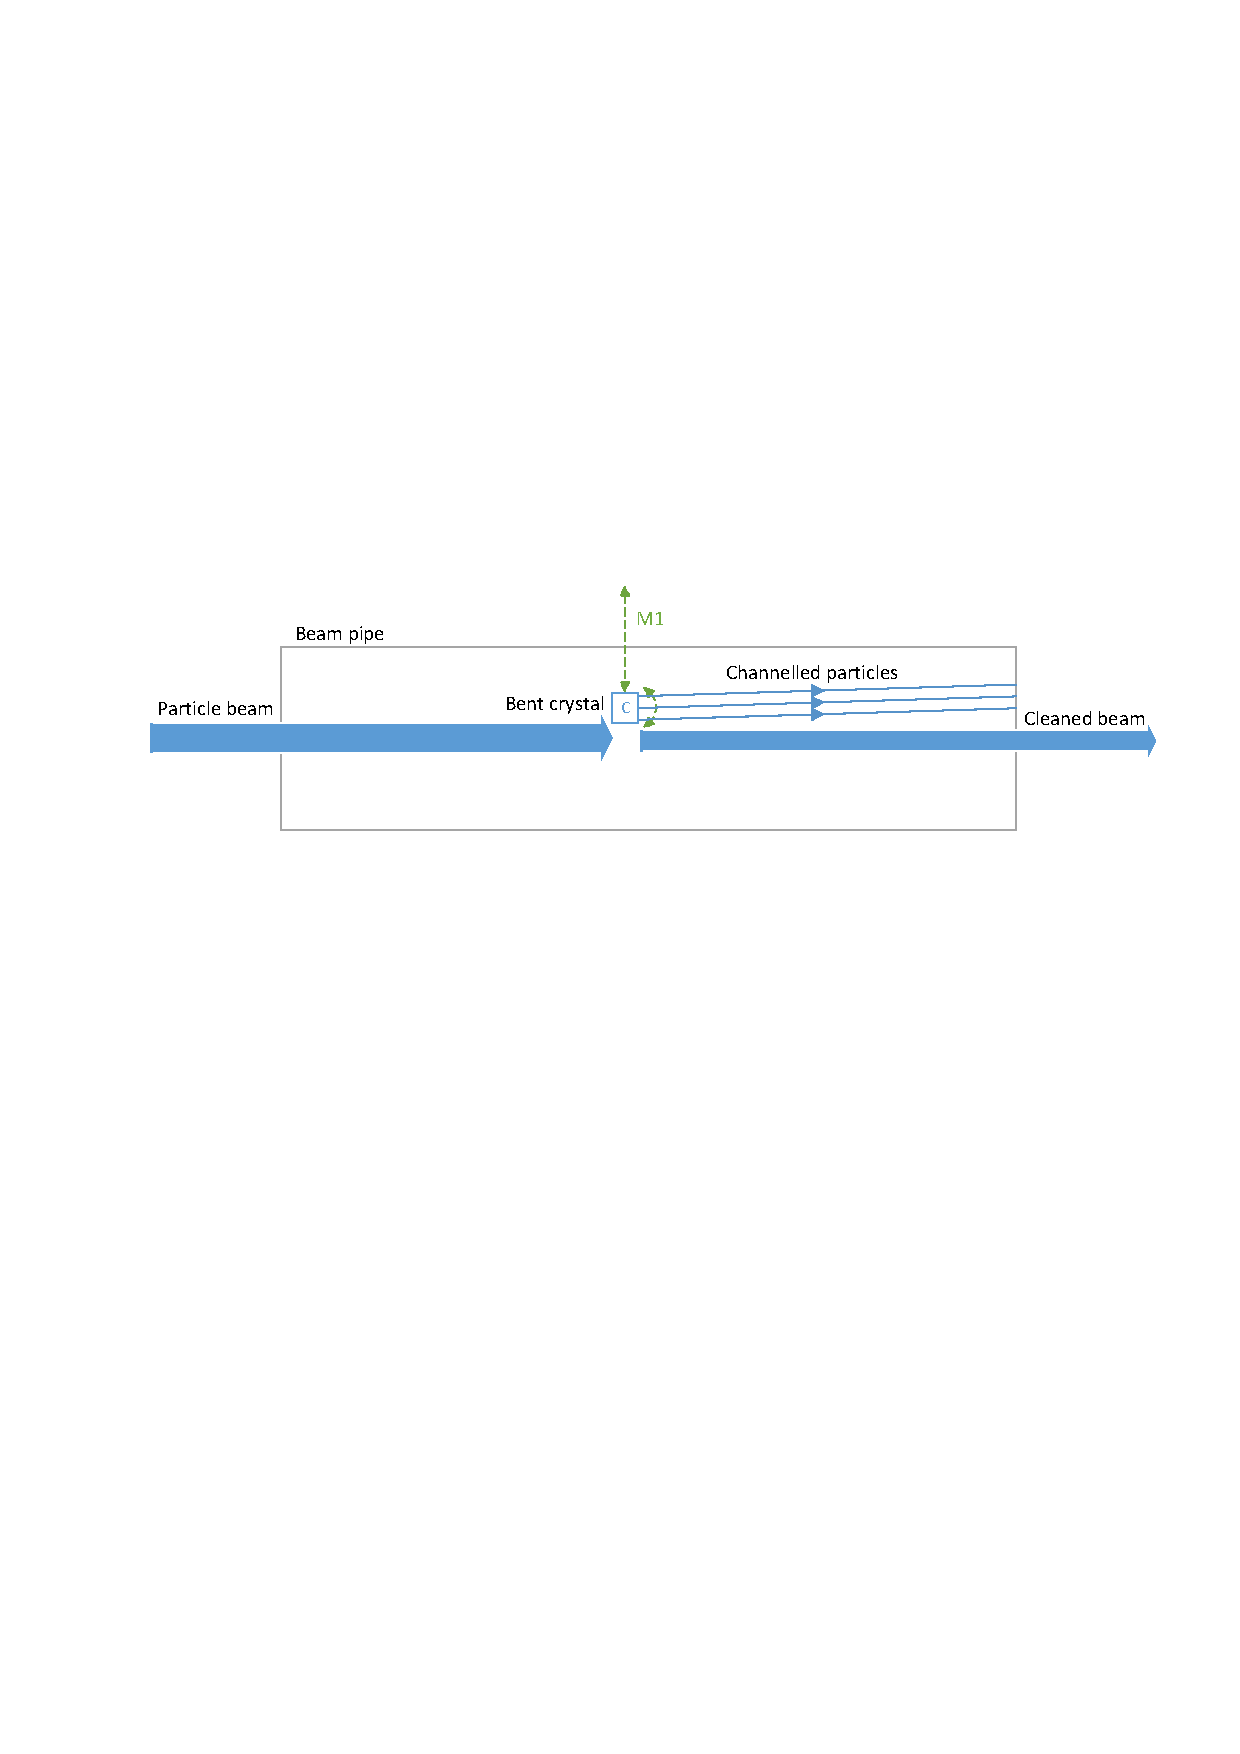
\includegraphics[width=1\textwidth, trim= 2cm 15cm 1cm 10cm, clip=true]{fig/matlab/collimation}
  \caption{\label{fig:collimation}Illustration of the crystal collimation principle as seen from above. The green dashed line represents the linear and the rotational stage movement.}
\end{figure}

The block named "C" represents the bent crystal which can be moved into the beam by the linear stage and rotated by the rotational stage that is attached to the linear axis. The crystal's linear and rotational movement are indicated in the figure as green dashed lines. During operation, physicists will drive the crystal close to the beam, enter it with an angle and rotate it slightly (in the range of \unit{1}{\milli\rad}) until the channeling effect is detected. Channeled particles (illustrated as arrowed lines in Figure~\ref{fig:collimation}) will then bend off from the beam core to be absorbed further down the beam pipe.

The collimator unit consists of a T-shape structure containing two linear and one rotational stage, as partly illustrated in Figure~\ref{fig:goniometer}.

\begin{figure}[h]
  \centering %crop: left bottom right top
  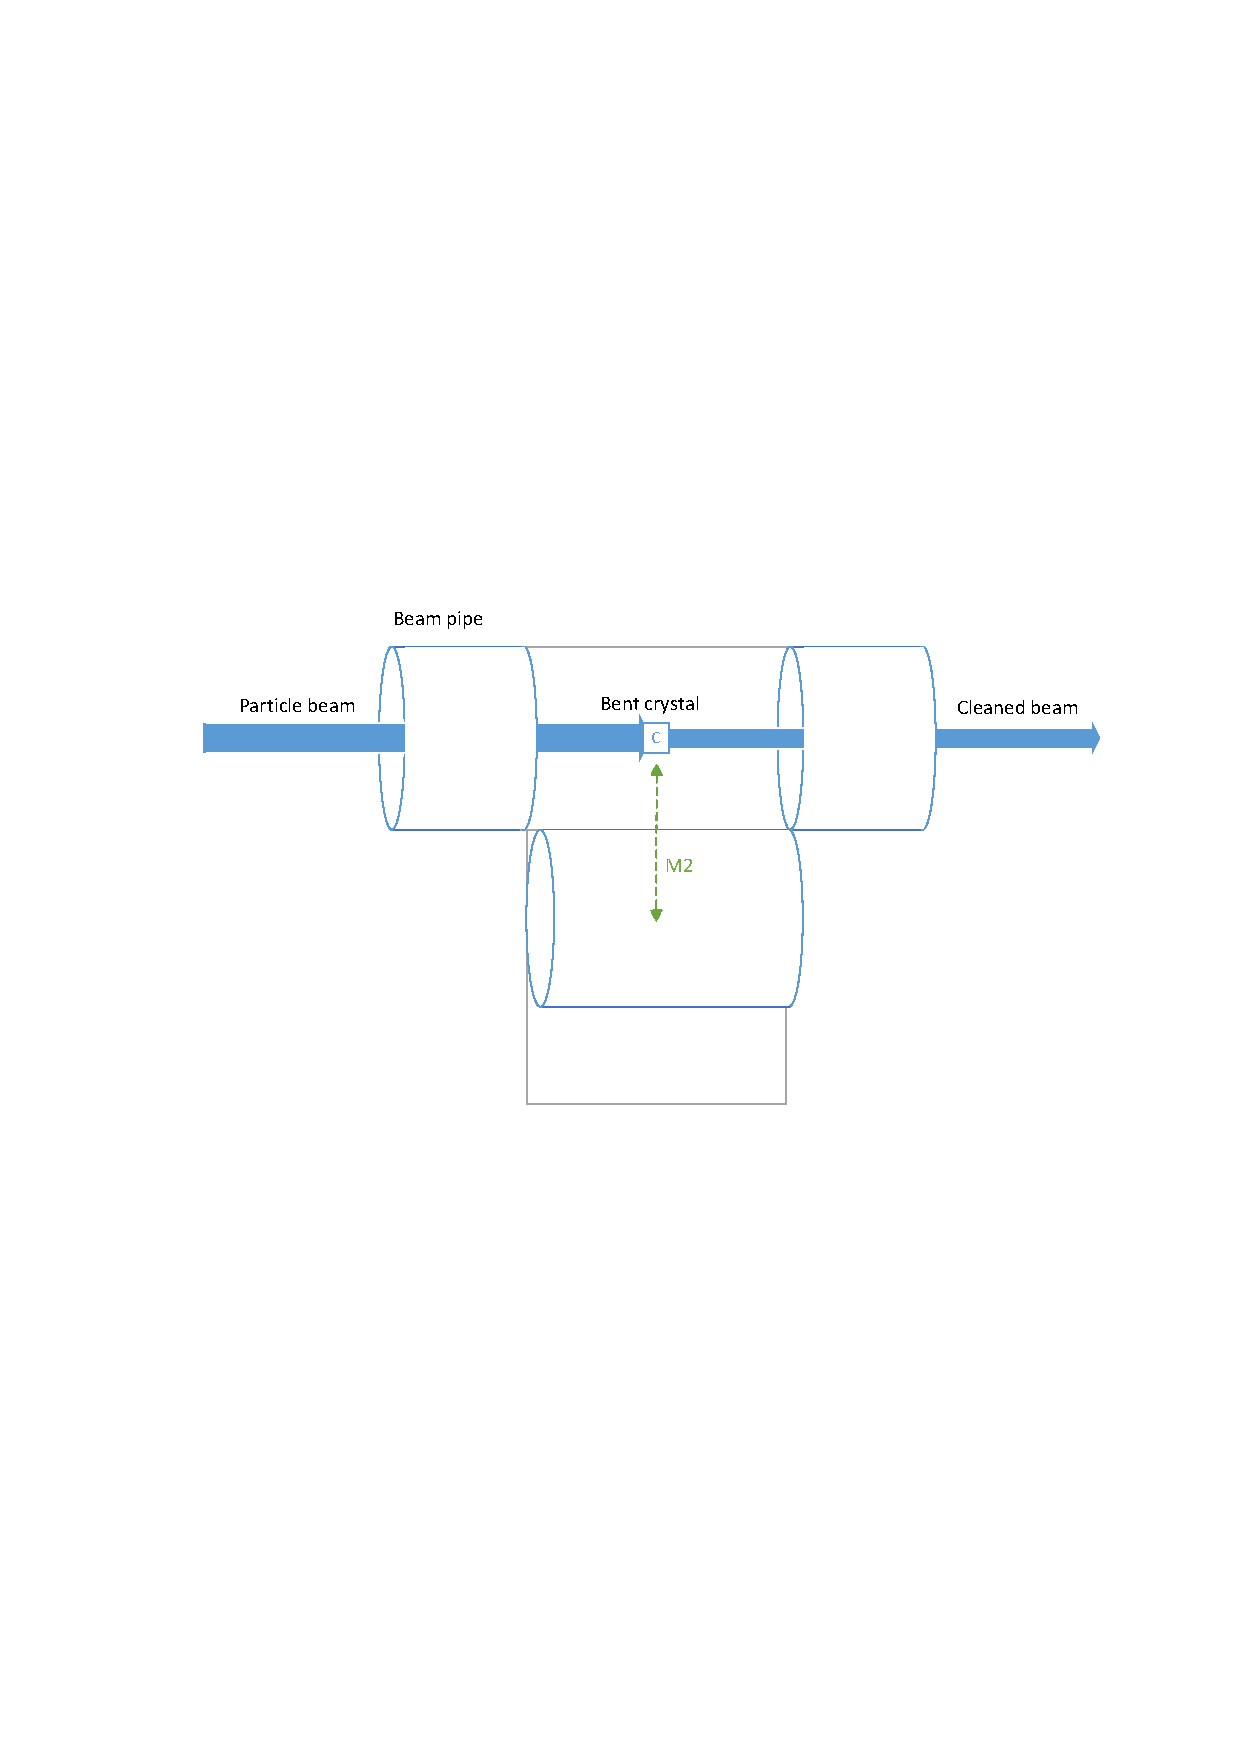
\includegraphics[width=1\textwidth, trim= 2cm 12cm 1cm 10cm, clip=true]{fig/matlab/goniometer}
  \caption{\label{fig:goniometer}Illustration of the crystal collimation principle as seen from the side. The green dashed line represents the movement of the beam pipe piece.}
\end{figure}

Each linear stage is driven by a stepping motor, labeled as \emph{M1} in Figure~\ref{fig:collimation} and \emph{M2} in Figure~\ref{fig:goniometer}, separately controlled in open-loop by an individual drive unit. The motor driving the vertical axis, \emph{M2}, is used to move a piece of beam pipe inside the T-shape, giving access to the crystal to enter and to close it when the collimation system is out of operation. This movement is illustrated in Figure~\ref{fig:goniometer} with a green dashed line.

Figure~\ref{fig:collimator} shows the new collimator. In the top view the rotational and the linear horizontal stage is indicated by labels. In this figure, the rotational stage is in its outer position. During operation it will be pushed forward by the linear axis into the beam pipe. Figure~\ref{fig:collimator-through} shows the inside of the beam pipe during movement of the beam pipe piece, the same movement that Figure~\ref{fig:goniometer} is illustrating. In Figure~\ref{fig:collimator-mirror} the crystal support has been injected into the beam pipe, note that the crystal itself is in this picture replaced by a small circular mirror.

\begin{figure}[tpb]
  \centering %crop: left bottom right top
  \subfloat[][\label{fig:collimator-side}Side view]{
  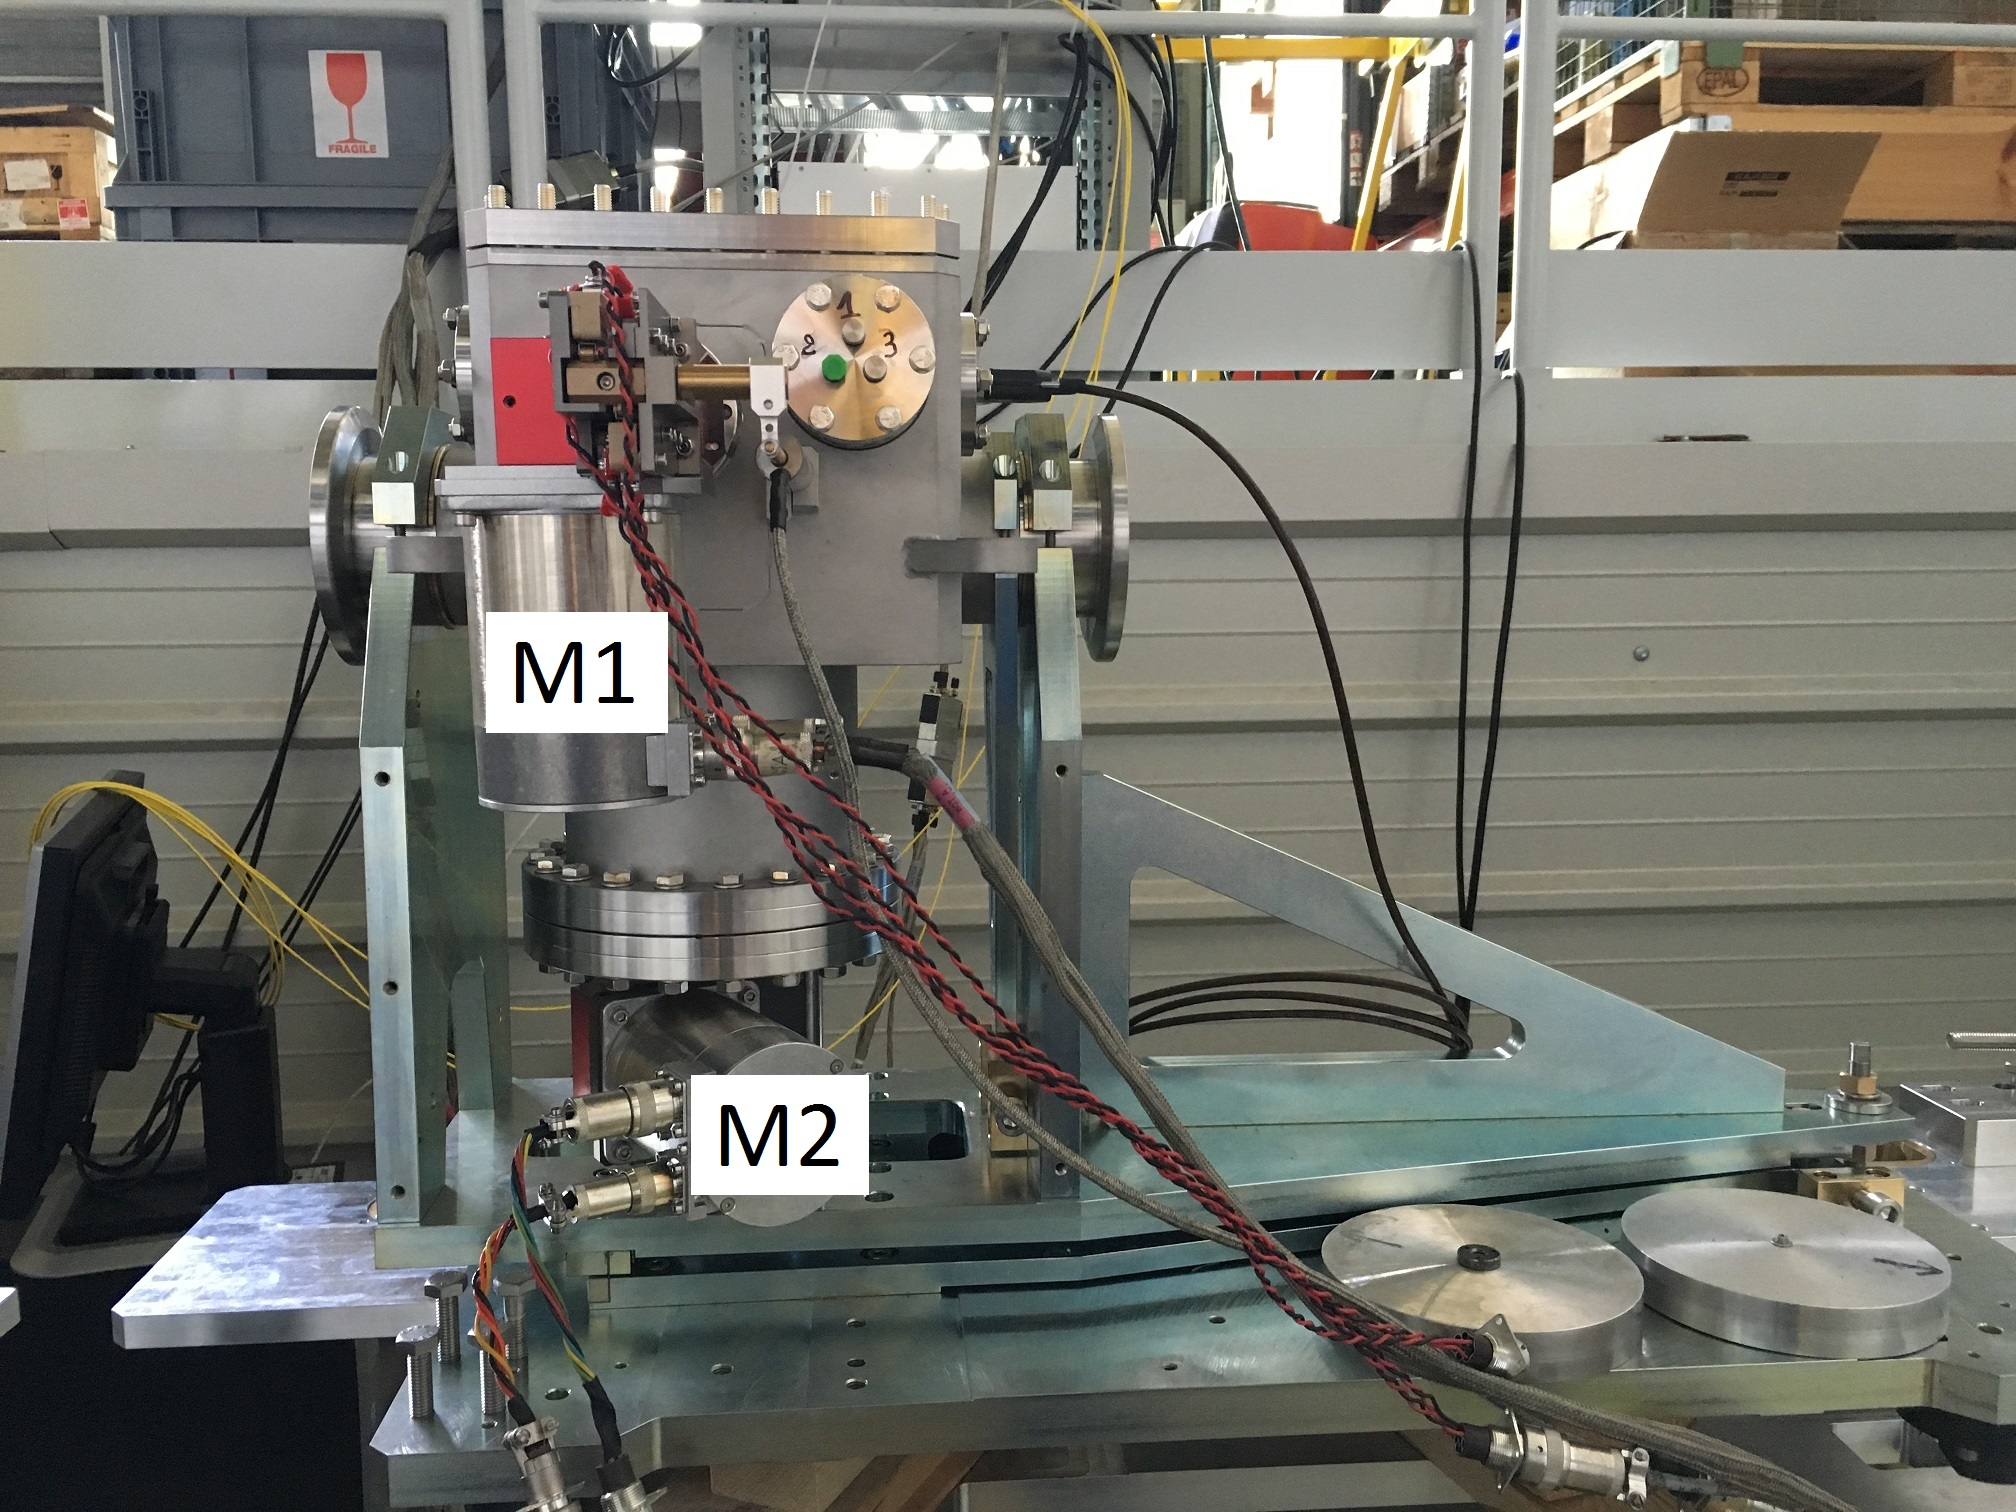
\includegraphics[width=0.5\textwidth, trim=2cm 11cm 2cm 5cm, clip=true]{fig/collimator-side}}
  \qquad
  \subfloat[][\label{fig:collimator-top}Top view]{
  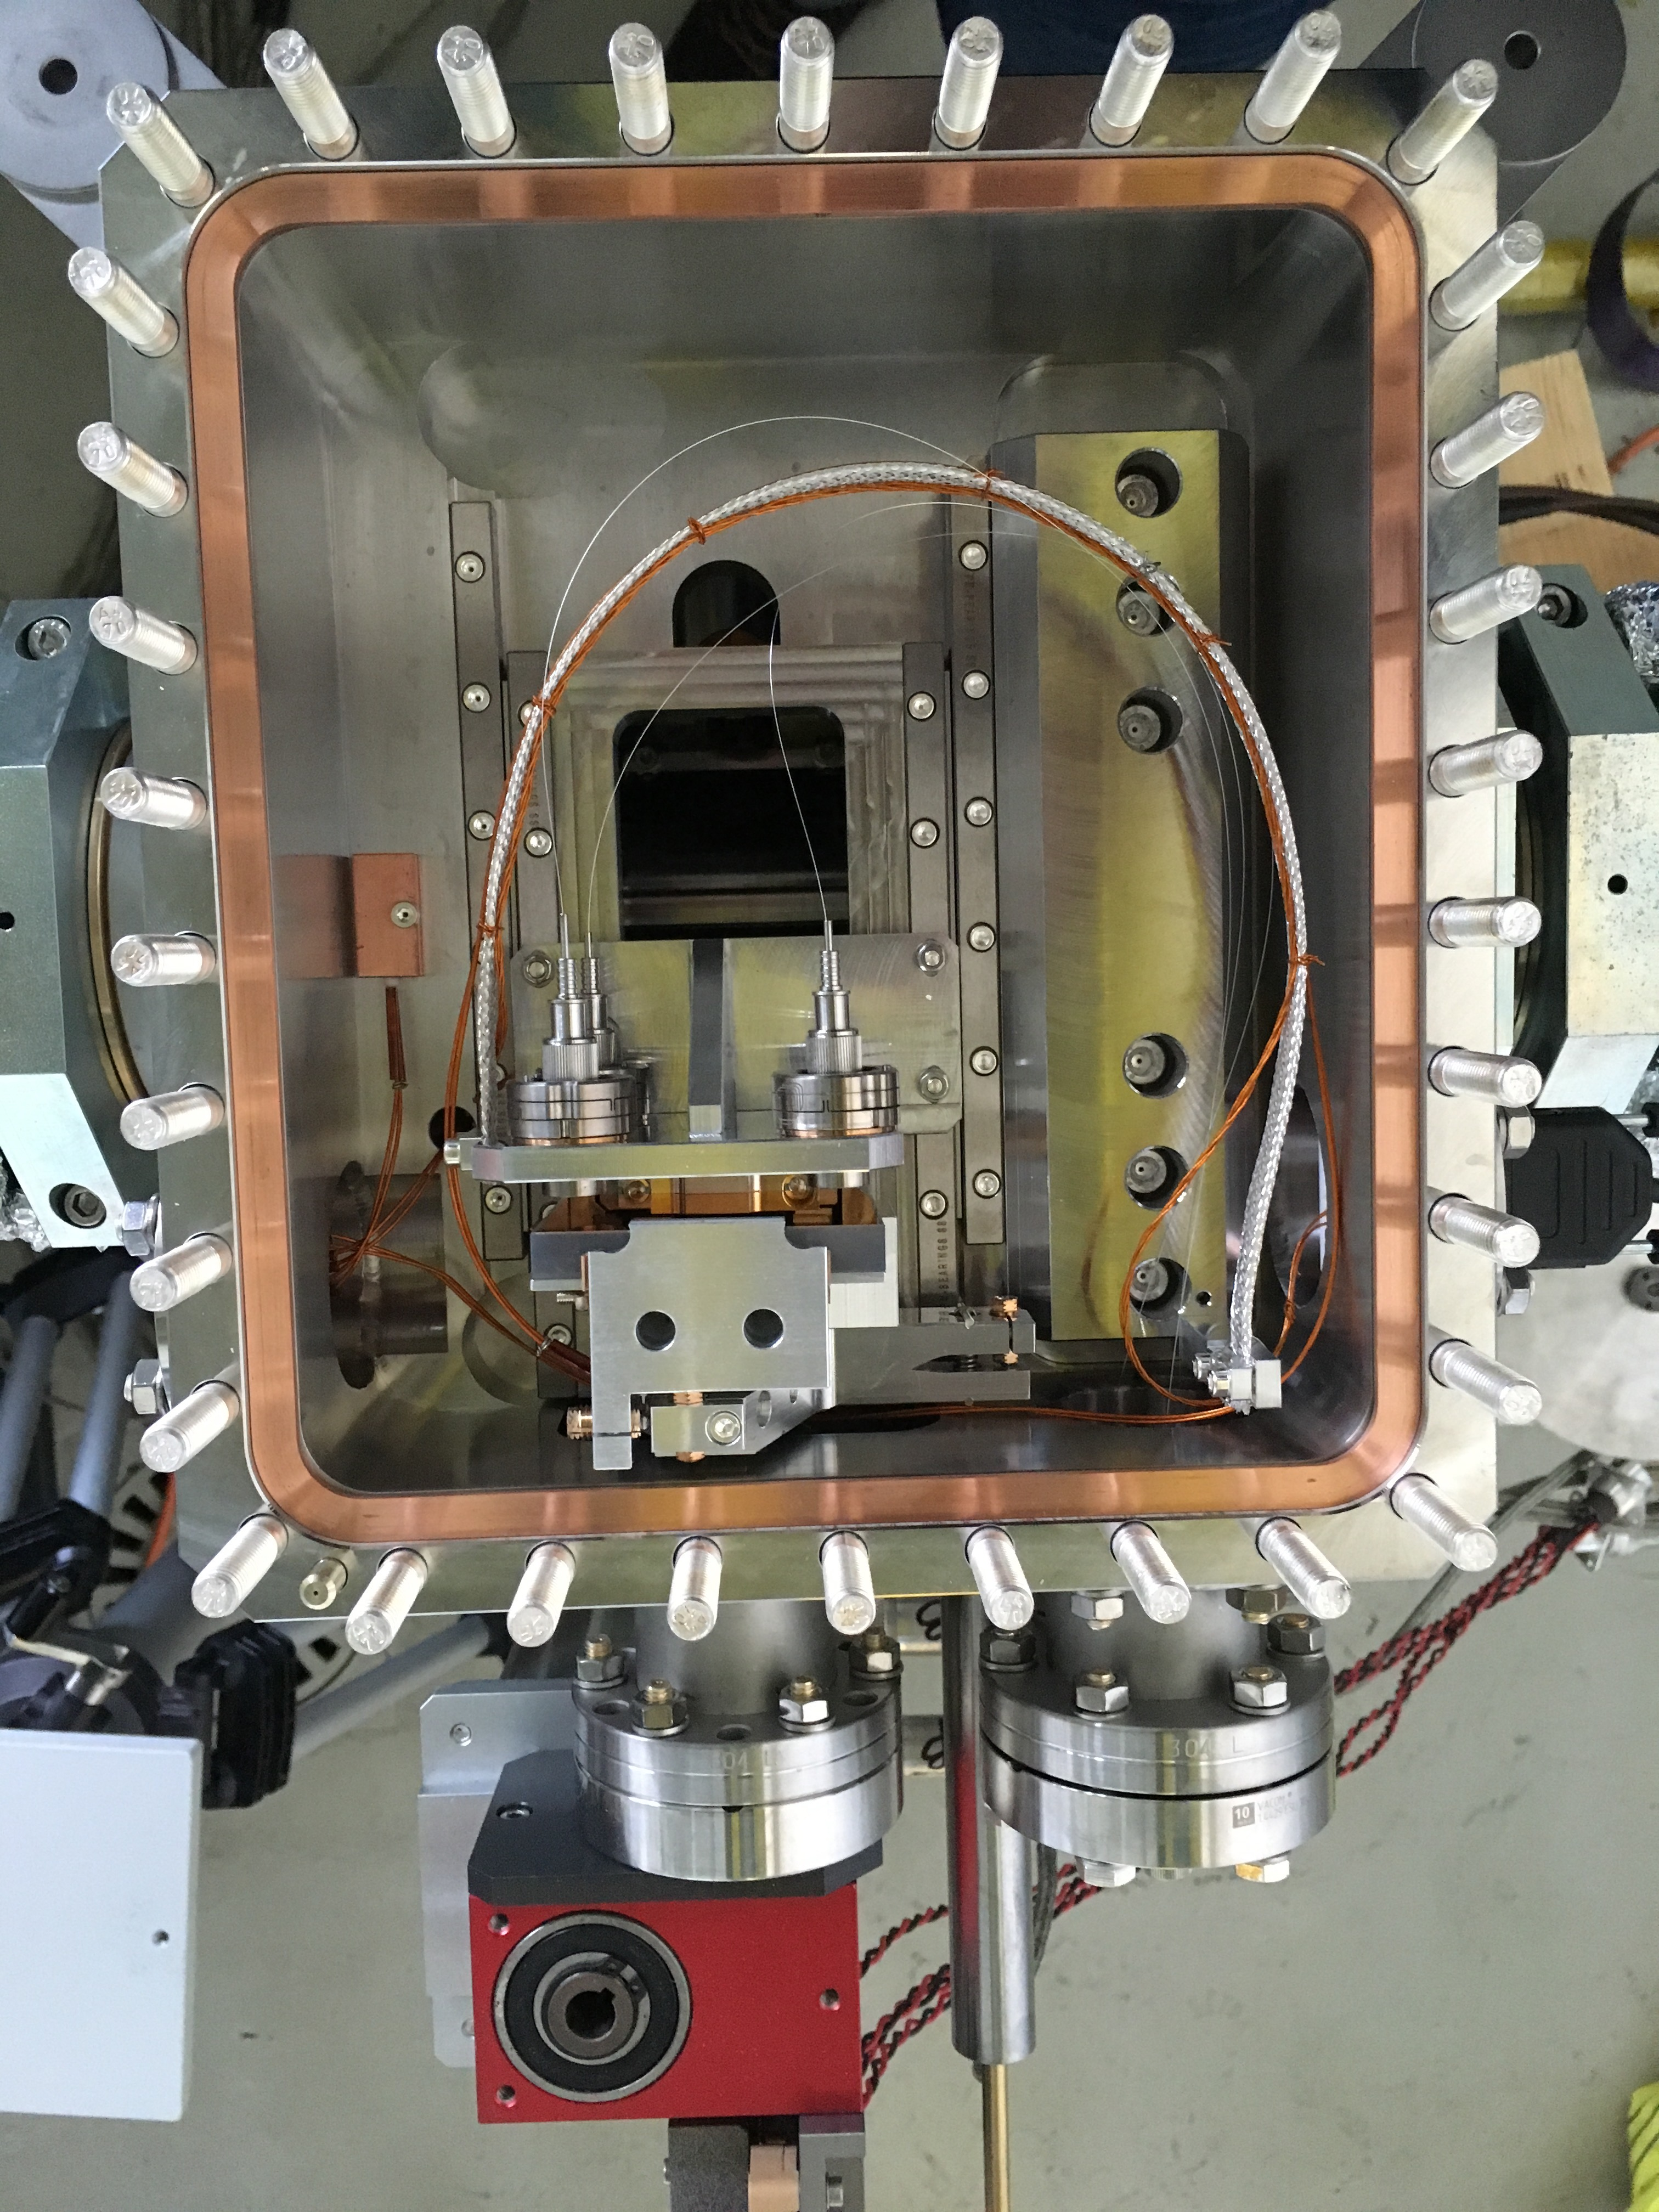
\includegraphics[width=0.42\textwidth, trim=0cm 0cm 0cm 0cm, clip=true]{fig/collimator-top}}
  \caption{\label{fig:collimator} The new collimator from the side (a) and the top (b).}
\end{figure}

\begin{figure}[tpb]
  \centering %crop: left bottom right top
  \subfloat[][\label{fig:collimator-through} Giving access]{
  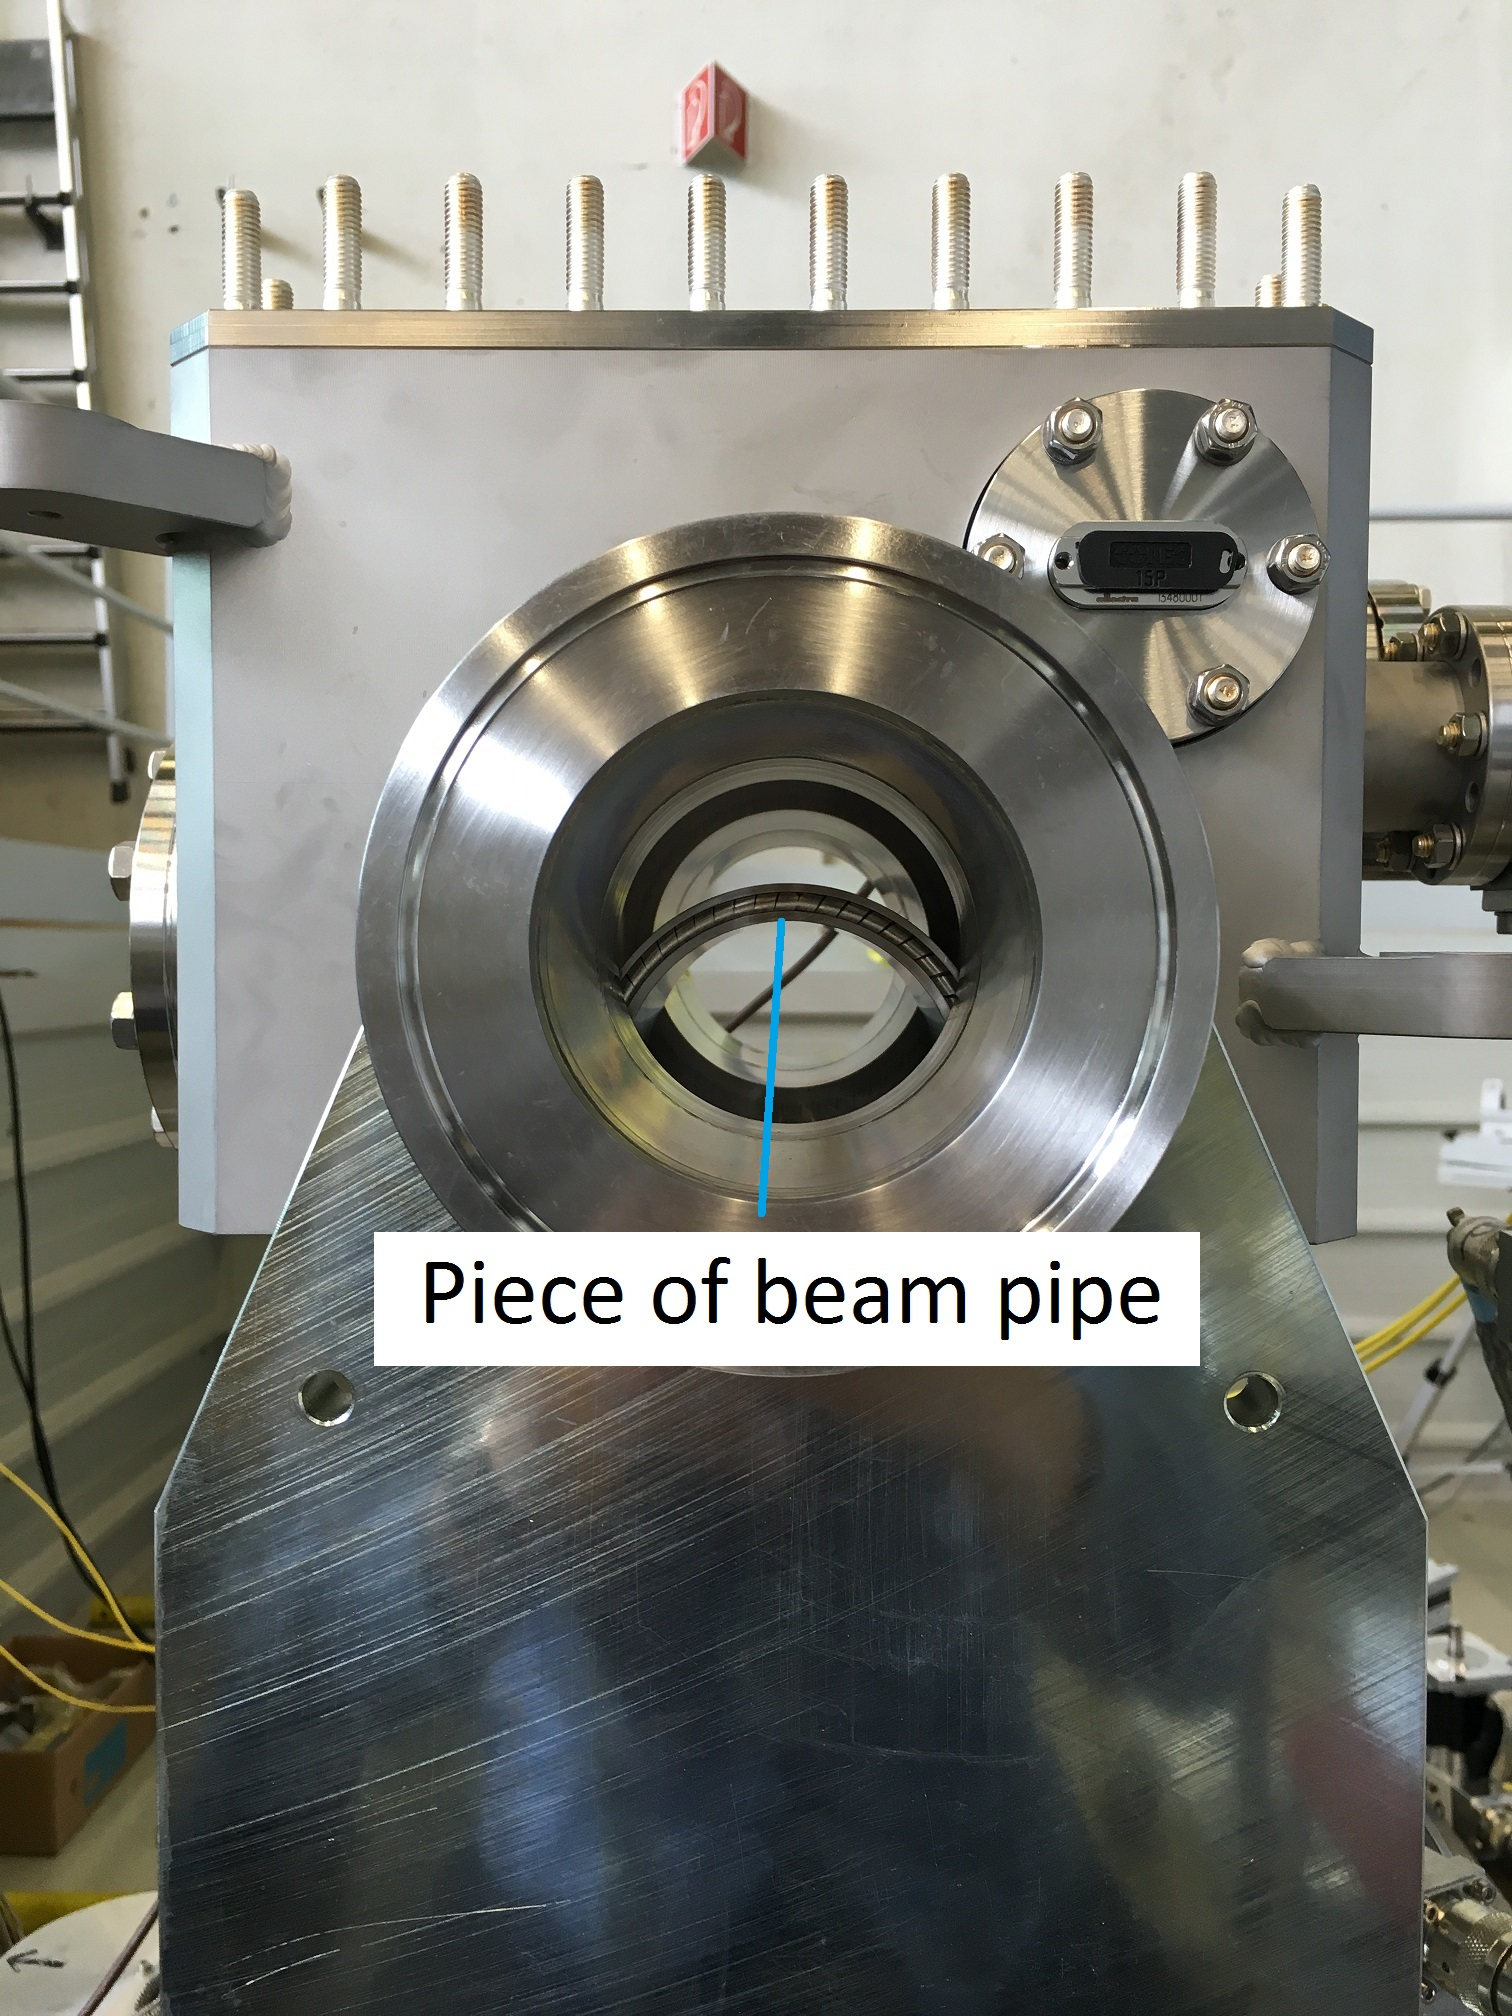
\includegraphics[width=0.42\textwidth, trim=3cm 12.8cm 2cm 5cm, clip=true]{fig/collimator-through}}
  \qquad
  \subfloat[][\label{fig:collimator-mirror} Insertion of crystal]{
  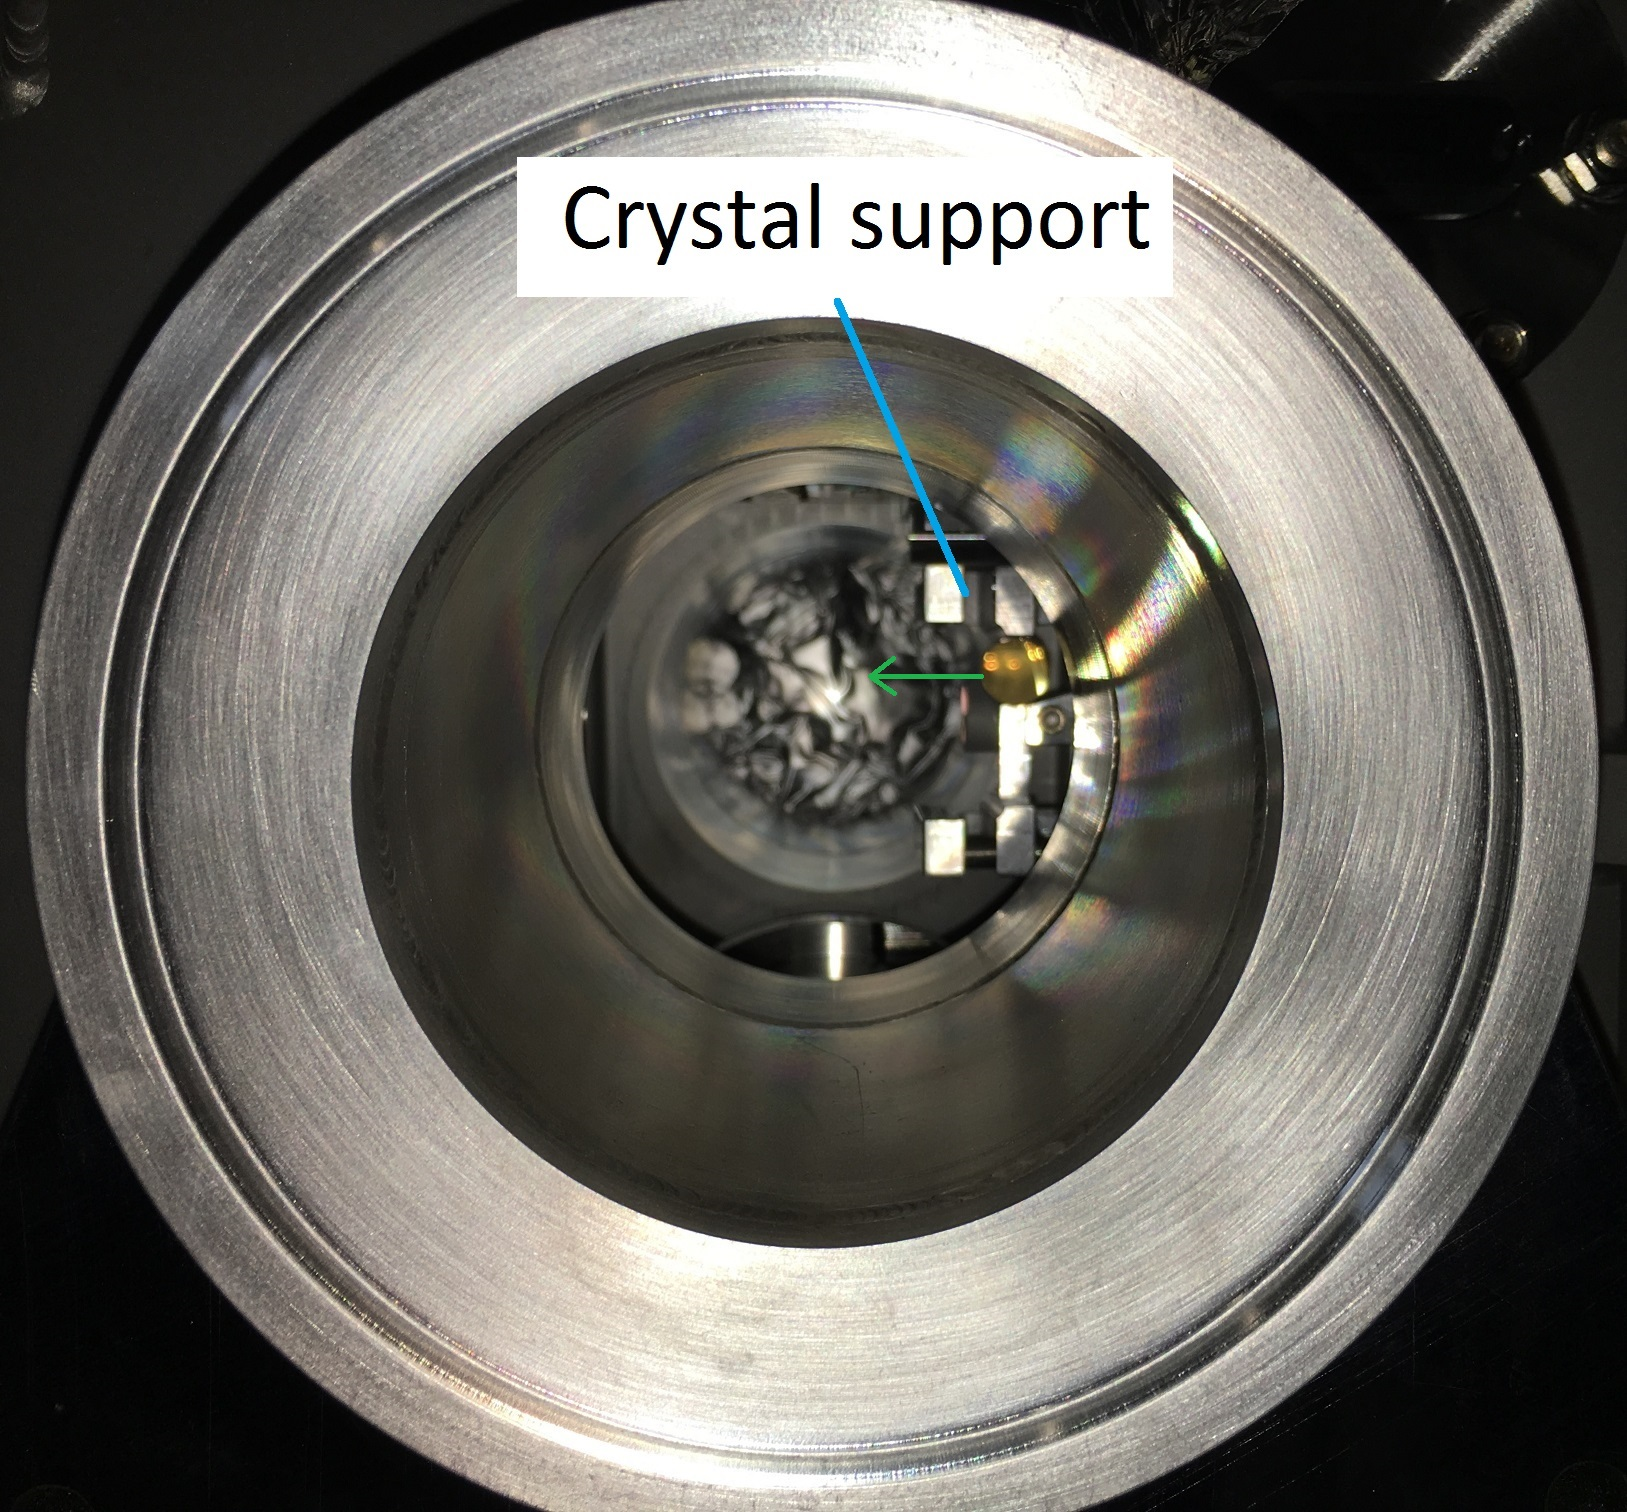
\includegraphics[width=0.5\textwidth, trim=0cm 0cm 0cm 0cm, clip=true]{fig/collimator-mirror}}
  \caption{\label{fig:collimator-t} The new collimator with the beam pipe piece half-way out (a) and the crystal inserted into the beam pipe (b).}
\end{figure}

\FloatBarrier
\section{Rotational stage}
\label{sec:rotational_stage}
The rotational stage as shown in Figure~\ref{fig:rotationalstage} is composed by a monolithic amplifying structure, a prestressed piezoelectric stack actuator and an interferometer measurement system. The flexure-hinge based structure, avoids sliding parts and thereby enhance precision by reducing the number of nonlinear effects (e.g. backlash and friction). A piezoelectric stack actuator is exploited to generate the rotational movement by interacting on a amplifying lever that applies the force on the rotational head a few millimeters from the center of rotation, marked as a red "X" in the picture. This amplifying structure gives the rotational stage a range of \unit{20}{\milli\rad} from a nominal linear range of \unit{40}{\micro\meter}.  The \abbrPEA is prestressed in order to enhance the overall stiffness as well as keeping the stack in place (the stack is non-glued to be sufficient in a radioactive area). This combination leads to a clear resonant structure, due to the characteristics of the \abbrPEA and the flexible structure, demanding a properly designed controller.

\begin{figure}[h!]
  \centering
  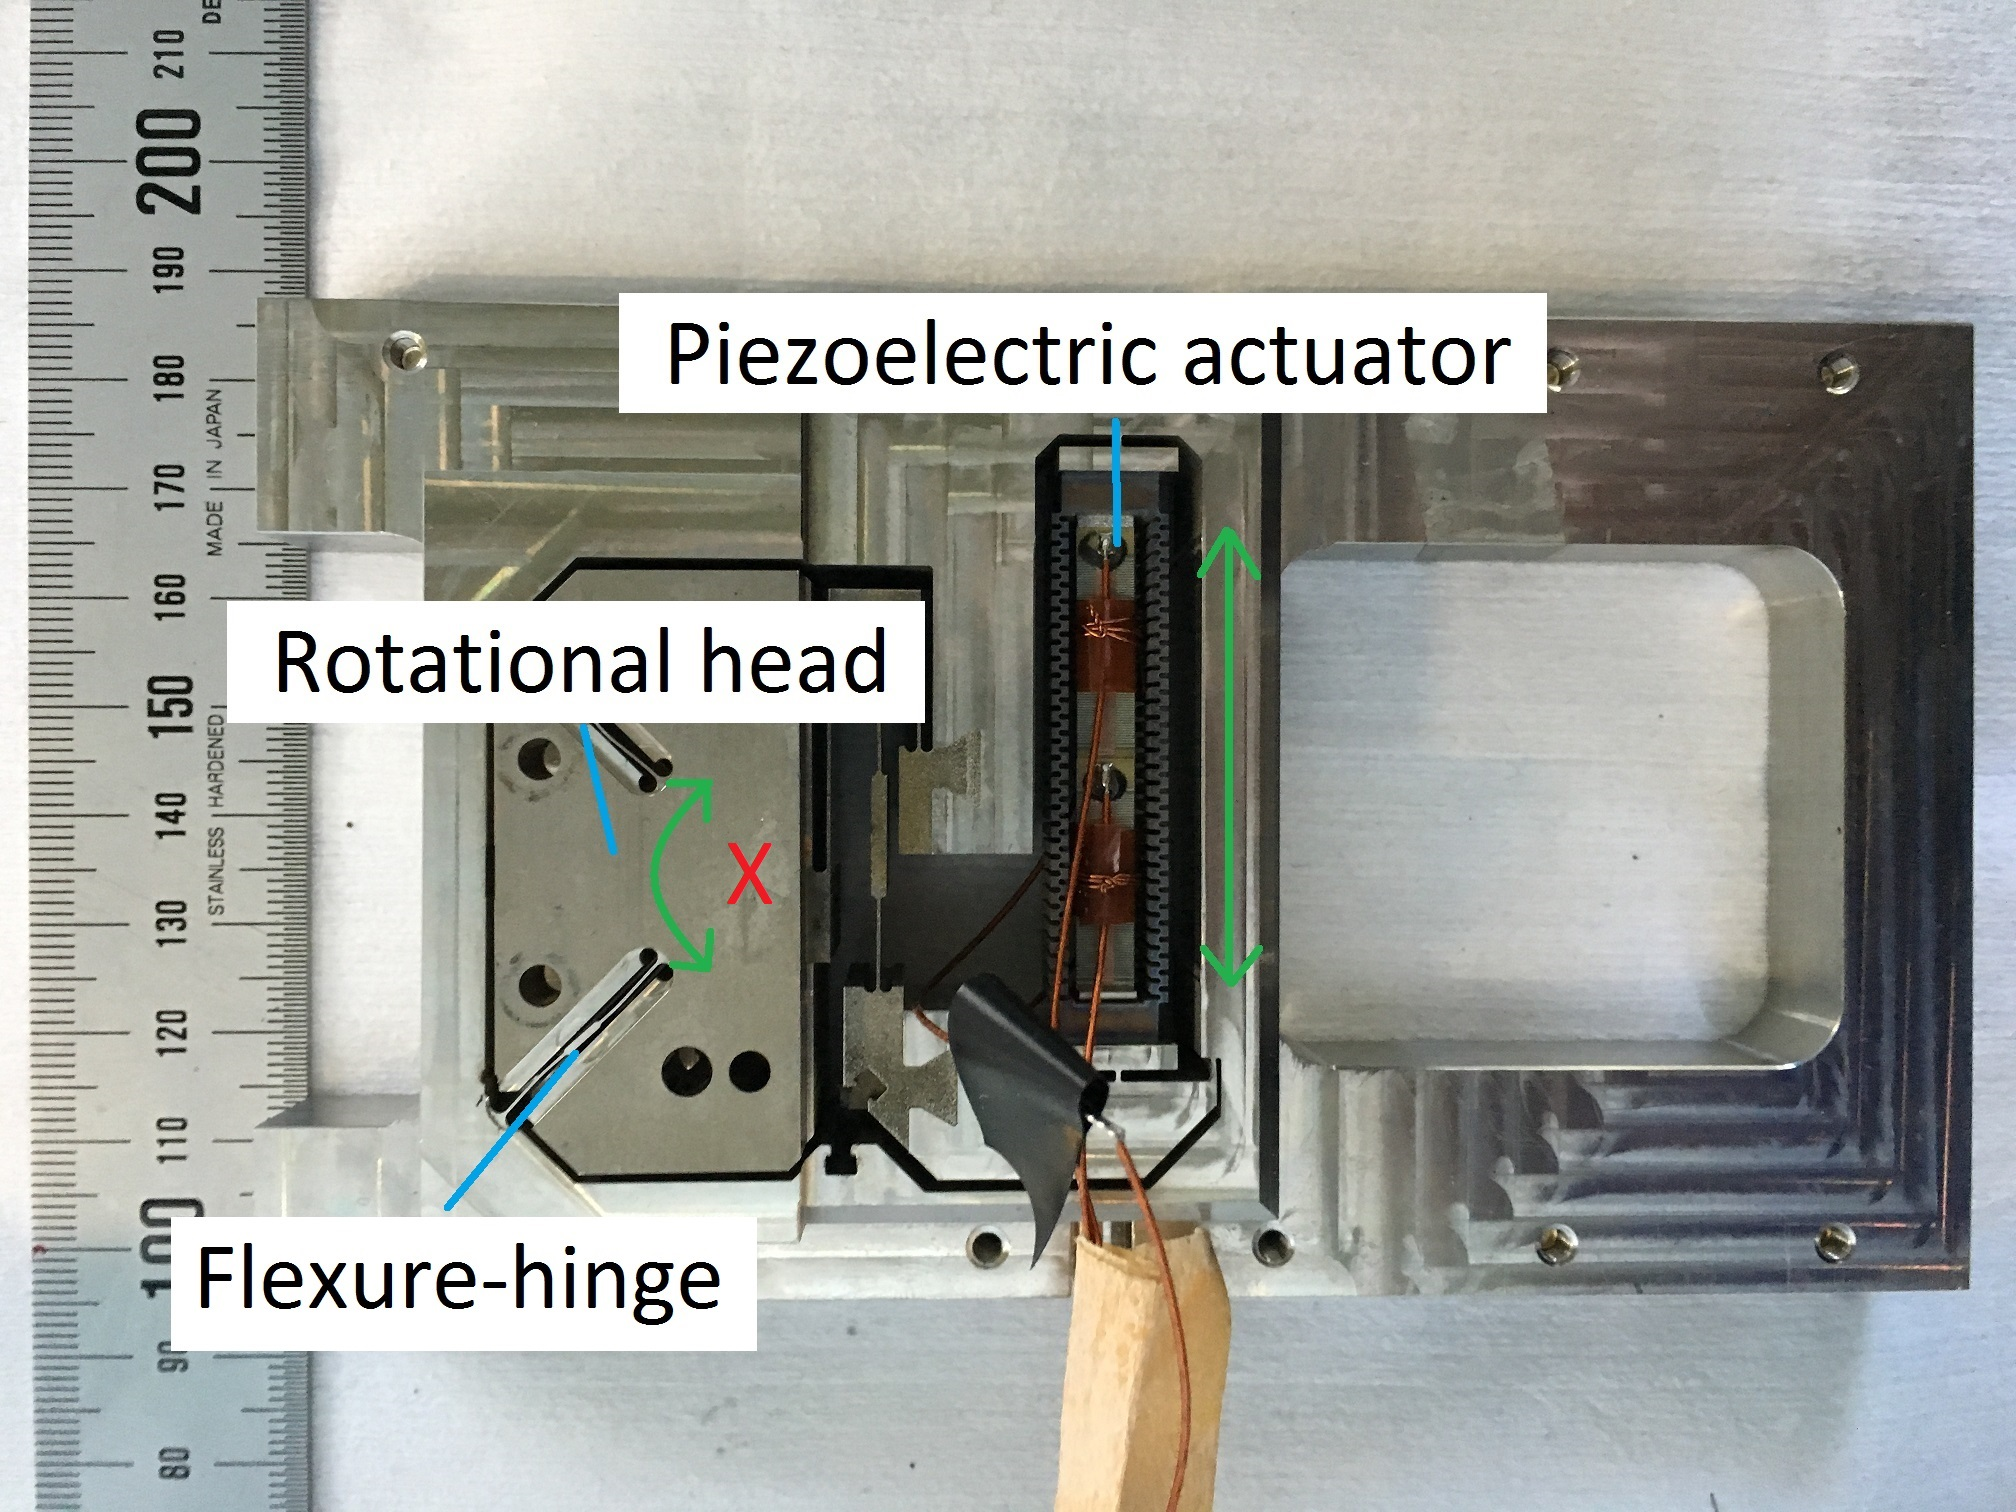
\includegraphics[width=0.7\textwidth]{fig/rotational-stage.jpg}
  \caption{\label{fig:rotationalstage} Piezo-actuated rotational stage used in the new collimator.}
\end{figure}

For the measurement system, three interferometric heads are placed on top of the rotational stage as seen Figure~\ref{fig:rotationalstage-side}, pointing towards a mirror that is attached to the crystal support and to the rotational head, perpendicular to the plane of rotation. The setup allows for measurements of both the yaw and roll angle (the coordinate system is defined with respect to the beam), but only the yaw angle is used in the feedback to the rotational stage control loop. Note that the crystal is mounted below the rotational head and that only the top of the crystal support is shown in the picture.

\begin{figure}[h!]
  \centering
  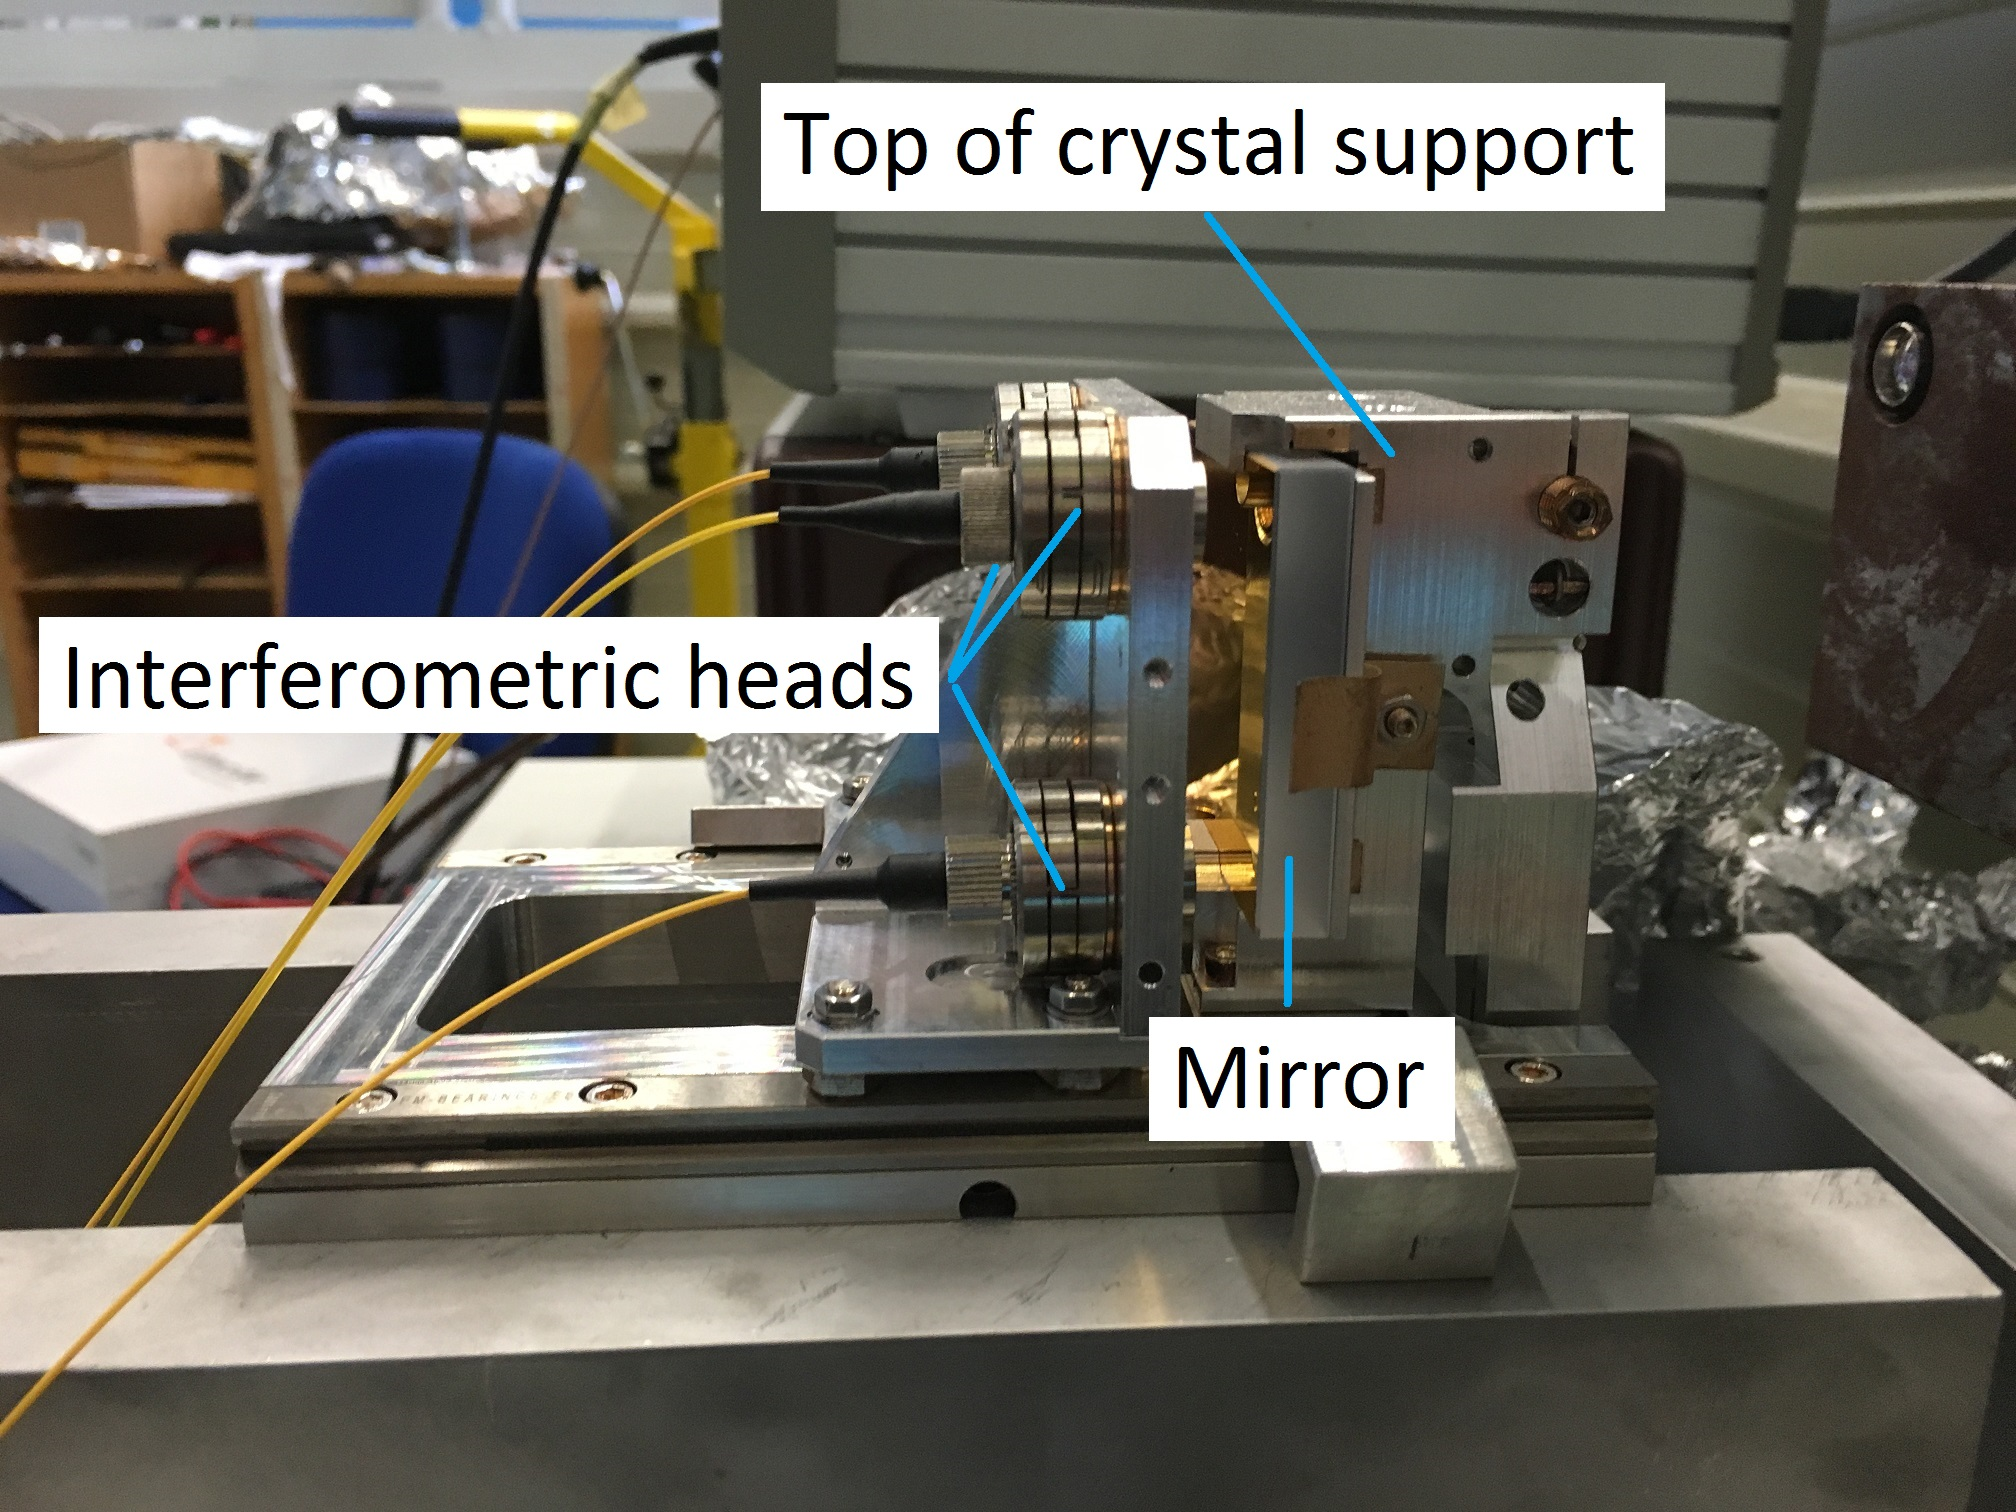
\includegraphics[width=0.7\textwidth]{fig/rotational-stage-interferometer.jpg}
  \caption{\label{fig:rotationalstage-side} Rotational stage with the crystal support and the interferometric system mounted on top.}
\end{figure}

\section{Piezoelectric Stack Actuators}
The rotational stage uses a linear piezoelectric stack actuator to create the movement. It provides a displacement range from 0 to \unit{30}{\micro\meter}, corresponding to -20 and +150V, respectively. The actuators are made of many thin, stacked electro-active ceramic disks, electrically connected in parallel. This construction allows for a high stiffness actuator that still can exhibit long displacement ranges \cite{Piezo:2008}.

\subsection{Hysteresis Effect}
The hysteresis effect is a nonlinear effect that is present during the operation of piezoelectric actuators. It occurs when the driving direction is reversed and origins from the polarization and the molecular effects in the piezo-ceramic. It depends on the amplitude of the applied voltage but also on the frequency of the input signal \cite{Qingson:2016}. Figure~\ref{fig:hysteresis} illustrates the hysteresis effect. One can see how the same voltage, e.g. 60V, corresponds to an angular position of \unit{5.2}{\micro\rad} in one direction and to \unit{7.2}{\micro\rad} in the opposite direction.

\subsection{Creep Effect}
The creep effect is another nonlinear effect that is present during the operation of piezoelectric actuators. The effect is a slow elongation or contraction of the actuator displacement over time with a constant driving signal and is caused by thermal effects in the piezo-ceramics. Figure~\ref{fig:creep} illustrates the creep effect. One can see how the rotational stage slightly drifts off from the reference after the applied negative step, increasing the tracking error over time.

\begin{figure}[h!]
  \centering %crop: left bottom right top
  \subfloat[][\label{fig:hysteresis} Hysteresis loop]{
  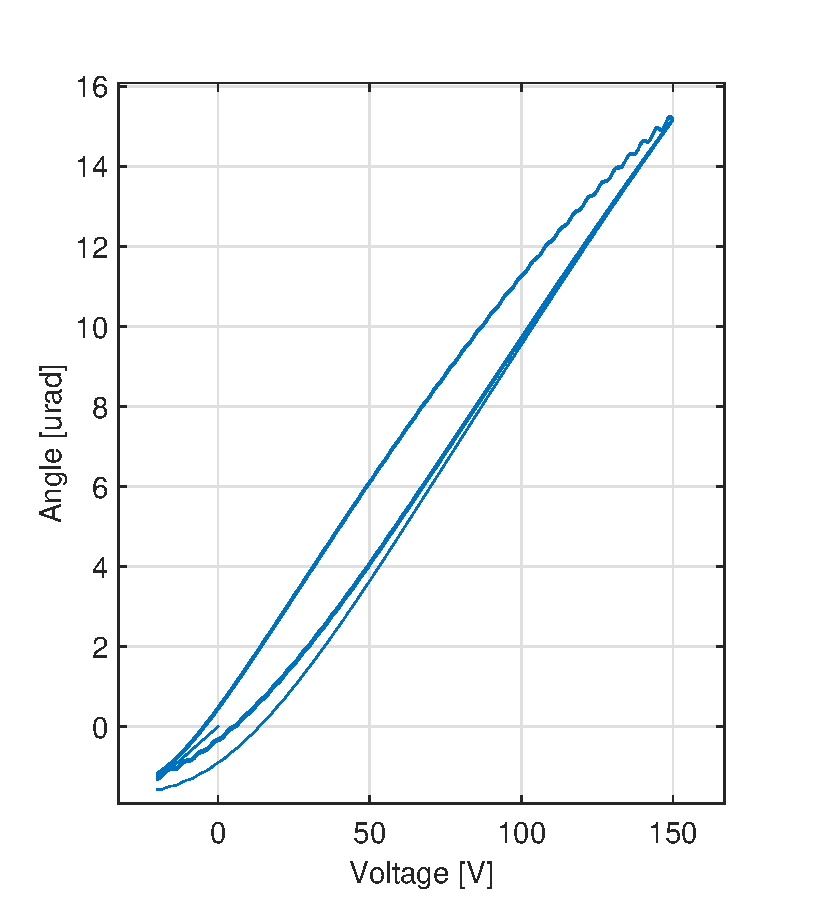
\includegraphics[width=0.46\textwidth, trim=0cm 0cm 1cm 0cm, clip=true]{fig/matlab/hysteresis.eps}}
  \qquad
  \subfloat[][\label{fig:creep} Creep effect]{
  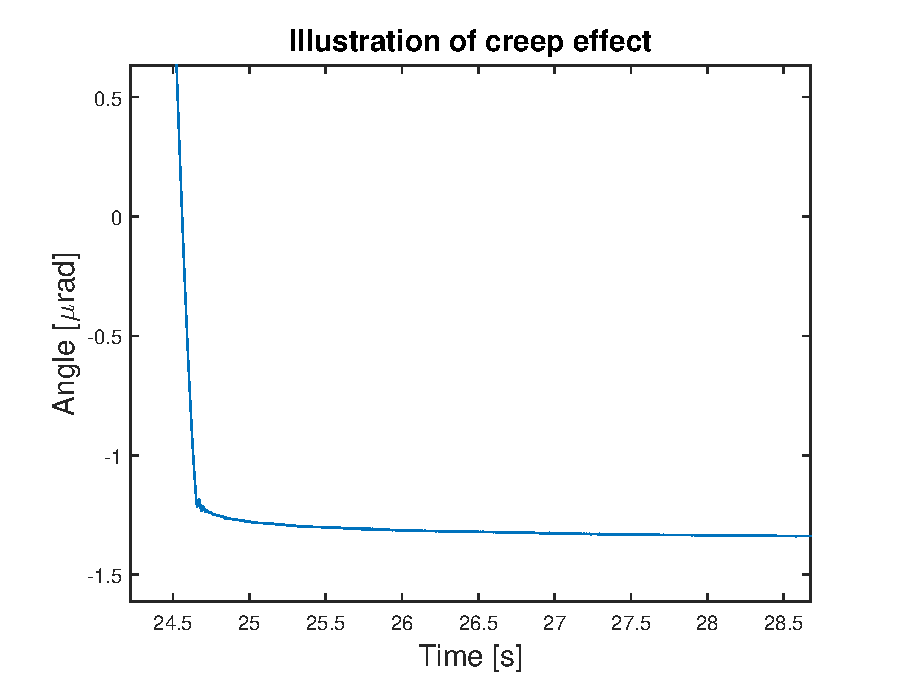
\includegraphics[width=0.46\textwidth, trim=0cm 0cm 1cm 0cm, clip=true]{fig/matlab/creep.eps}}
  \caption{\label{fig:effects} Illustration of the hysteresis effect (a) and creep effect (b). Note that the creep effect can last up to 10-15 minutes even if the plot only shows the development over 4 seconds.}
\end{figure}

The creep effect is in this project (and many others) efficiently suppressed by the feedback controller requiring no precise modeling and cancellation technique.

\section{Rotational Stage Modeling}
The piezo-actuated rotational stage is modeled by a Hammerstein structure, adopted by the authors in \cite{ButcherController:2015}, allowing them in principal, to decouple the nonlinear hysteresis from the linear system dynamics. The employed Hammerstein structure is depicted in Figure~\ref{fig:hammerstein} and consists of a \emph{Static Hysteresis} (rate independent) model and a \emph{Linear Dynamics} model. {\abbrPEA}s are known to show hysteretic behavior with a nonlocal memory (the current output does not only depend on the current input voltage but also on its history) as described in \cite{ButcherIdentification:2015}. This behavior is modeled by a generalized Maxwell-slip compensation model, described in \ref{sec:maxwell}. The extracted linear dynamics is identified using the described procedure in \ref{sec:linsys}

\begin{figure}[h]
  \centering %crop: left bottom right top
  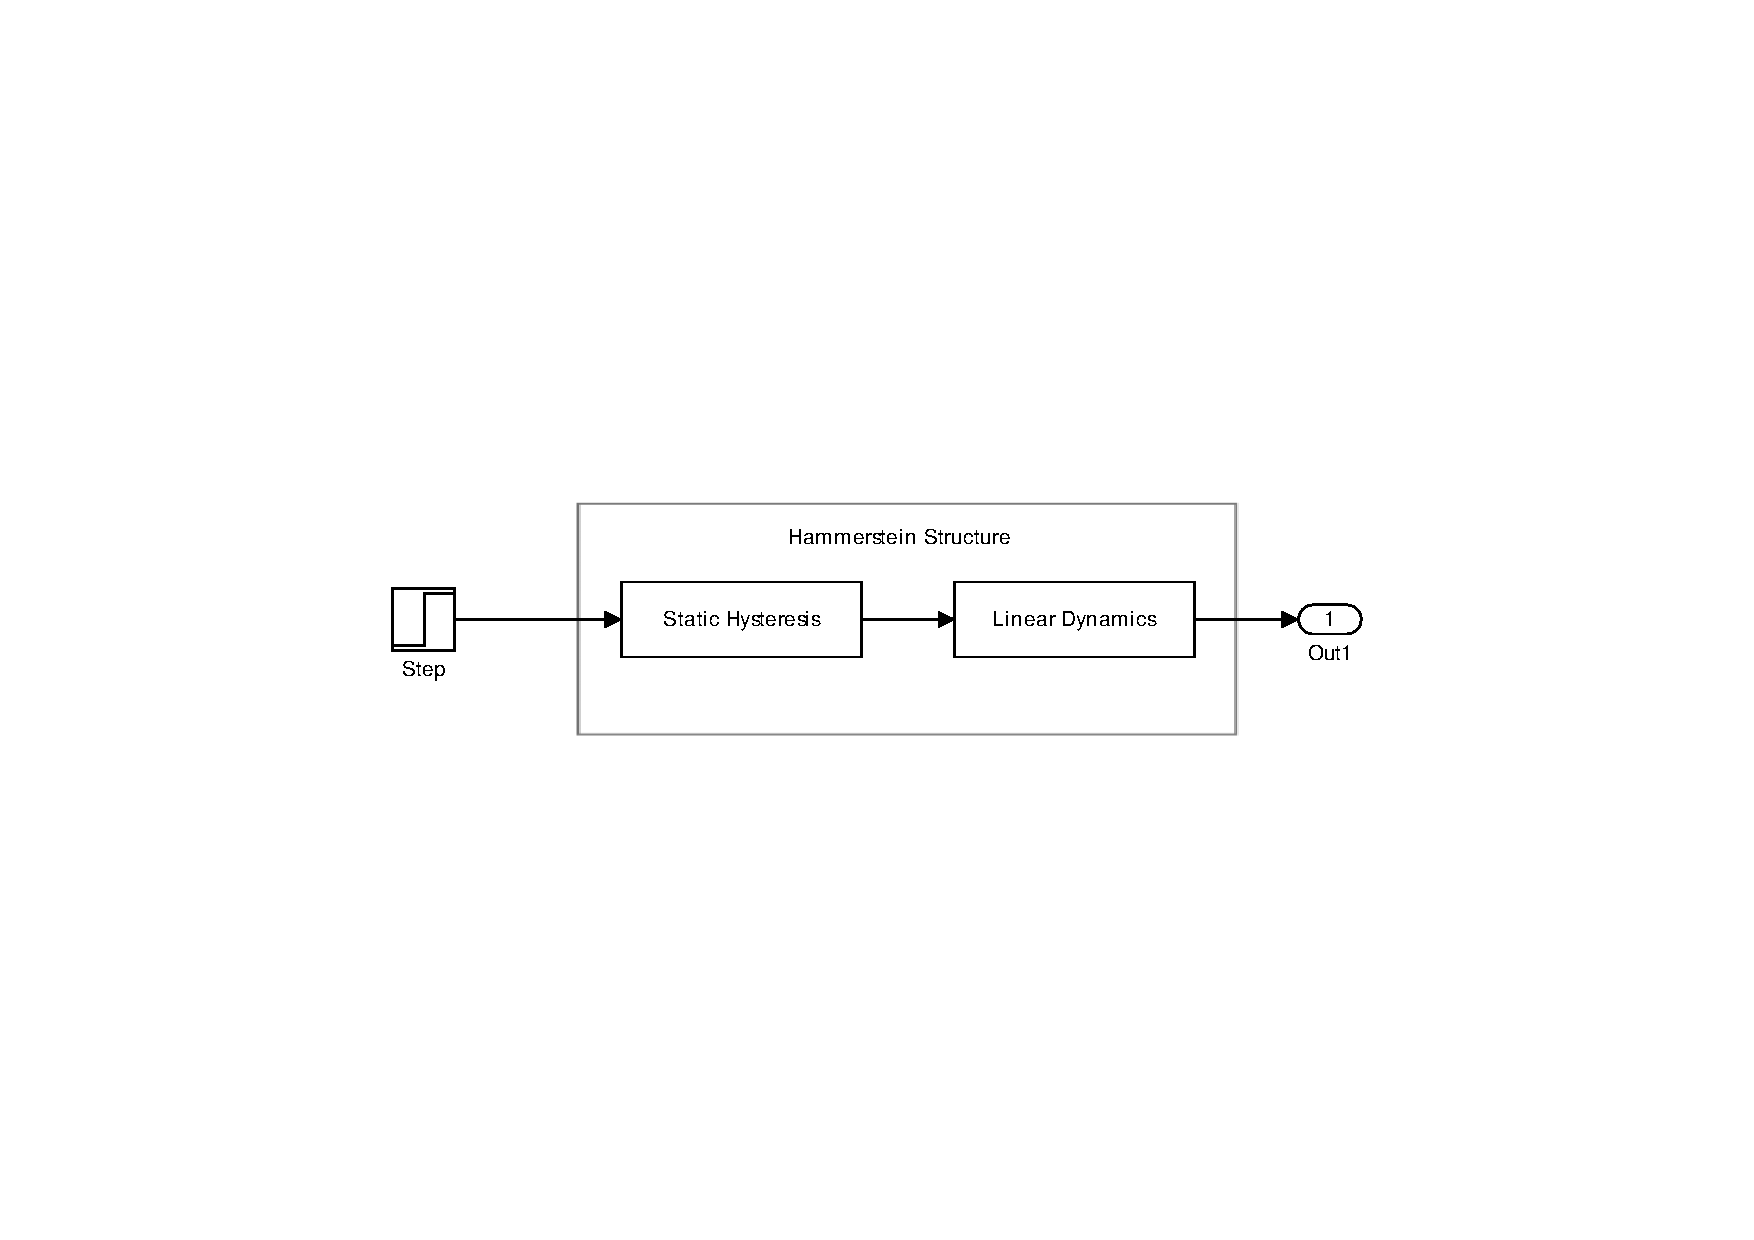
\includegraphics[width=0.7\textwidth, trim=8cm 8cm 7.73cm 8cm, clip=true]{fig/matlab/hammerstein}
  \caption{\label{fig:hammerstein}Block diagram of a Hammerstein structure, consisting of two blocks in series, modeling the static hysteresis and the linear dynamics, respectively.}
\end{figure}

\subsection{Maxwell-slip Model}
\label{sec:maxwell}
A generalized Maxwell-slip is used to model the hysteresis effect. It uses a parallel $n^{th}$ order elasto-slide element system with a friction force acting on each element, to create a nonlinear model. An elasto-slide element consist of a massless spring connected in series with a massless block that is subject to Coulomb friction. The inverse hysteresis model is summarized in the following equations and described more thoroughly in \citep{Ru:2016},

\begin{equation}
  \label{eq:maxwell_slip}
  F_i =
  \begin{cases}
    k_i(x - x_{bi}) & \quad \text{if }  k_i|x - x_{bi}| < f_i\\
    f_isgn(\dot{x}) \text{ and } x_{bi} = x - \frac{f_i}{k_i}sgn(\dot{x})  & \quad \text{else}\\
  \end{cases}
\end{equation}

\begin{equation}
  \label{eq:maxwell_sum}
  F = \displaystyle\sum_{i=1}^{n} F_i
\end{equation}

where $F_i$ is the output force, $k_i$ the spring constant, $f_i$ the break-away force and $x_b$ is the block position where $i=1 \hdots n$. In terms of the rotational stage $F_i$ represents the applied voltage, $x$ the input (rotational) displacement, $x_b$ angular position and $k_i, f_i$ are unknown parameters
The model parameters have been estimated by fitting the model to the major hysteresis loop, obtained by acquiring data from the system with a 0.5 Hz input driving signal as described in \citep{ButcherIdentification:2015,ButcherController:2015}. The identified set of parameters is presented in Table~\ref{tab:maxwell} where $n=10$. The model fit of the hysteresis model, which uses the same set of parameters as the inverse hysteresis model, is shown Figure~\ref{fig:maxwell}.

\begin{figure}[h]
  \centering
  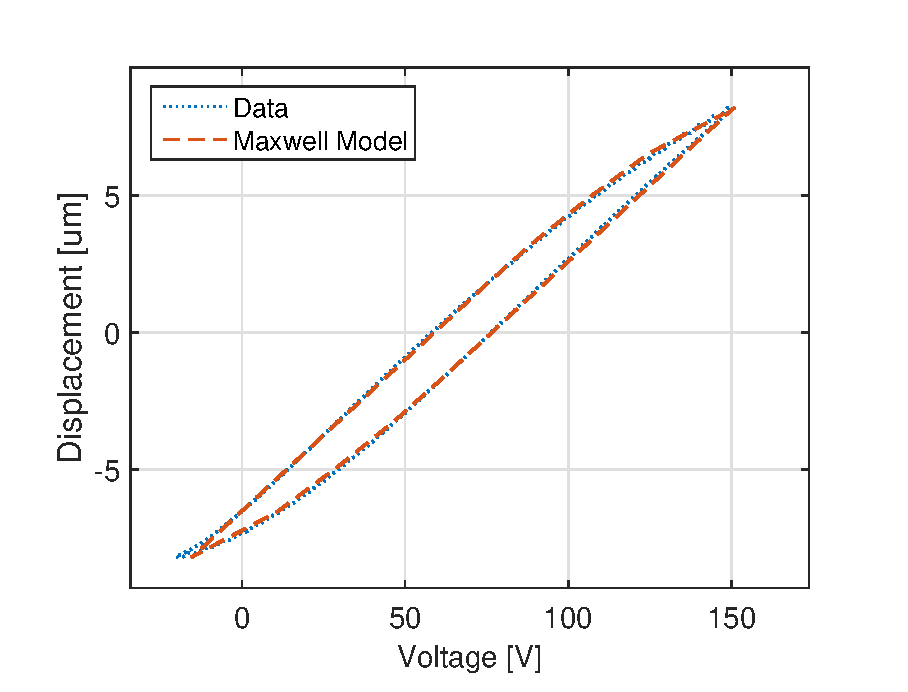
\includegraphics[width=0.7\textwidth]{fig/matlab/maxwell.eps}
  \caption{\label{fig:maxwell} The plot shows the model fit of the Maxwell slip model to the acquired hysteresis of the rotational stage. The fit has a mean squared error of 1.1464.}
\end{figure}

\begin{table}[h!]
  \centering
  \begin{tabular}{| l | l | l |}
    \hline
    $i$ & $k_i$ & $f_i$ \\ \hline
    1 & 4.53 & 3.69 \\
    2 & 0.90 & 1.46 \\
    3 & 1.01 & 2.47 \\
    4 & 0.36 & 1.16 \\
    5 & $1.49 \times 10^{-6}$ & $4.28 \times 10^{-6}$ \\
    6 & $2.89 \times 10^{-7}$ & $1.41 \times 10^{-6}$ \\
    7 & $1.59 \times 10^{-7}$ & $9.10 \times 10^{-7}$ \\
    8 & $1.39 \times 10^{-7}$ & $9.10 \times 10^{-7}$ \\
    9 & $2.28 \times 10^{-7}$ & $1.67 \times 10^{-6}$ \\
    10 & $4.58$ & 37.30 \\
    \hline
  \end{tabular}
  \caption{\label{tab:maxwell} Identified parameters of the Maxwell slip model.}
\end{table}

\subsection{Linear System Identification}
\label{sec:linsys}
The extracted linear dynamics have been identified as a $6^{th}$ order transfer function using a \abbrPRBS as excitation signal, allowing for a valid extraction from the nonlinear dynamics. The system transfer function has been derived in discrete-time using the System Identification Toolbox in Matlab. A more detail description of the procedure is available in \citep{ButcherController:2015}. Figure~\ref{fig:model} shows a comparison between the model and the real system in the frequency domain, where the Fast Fourier Transform (\abbrFFT) identification is calculated by taking the \abbrFFT of the output divided by the \abbrFFT of the input.
\begin{figure}[h]
  \centering
  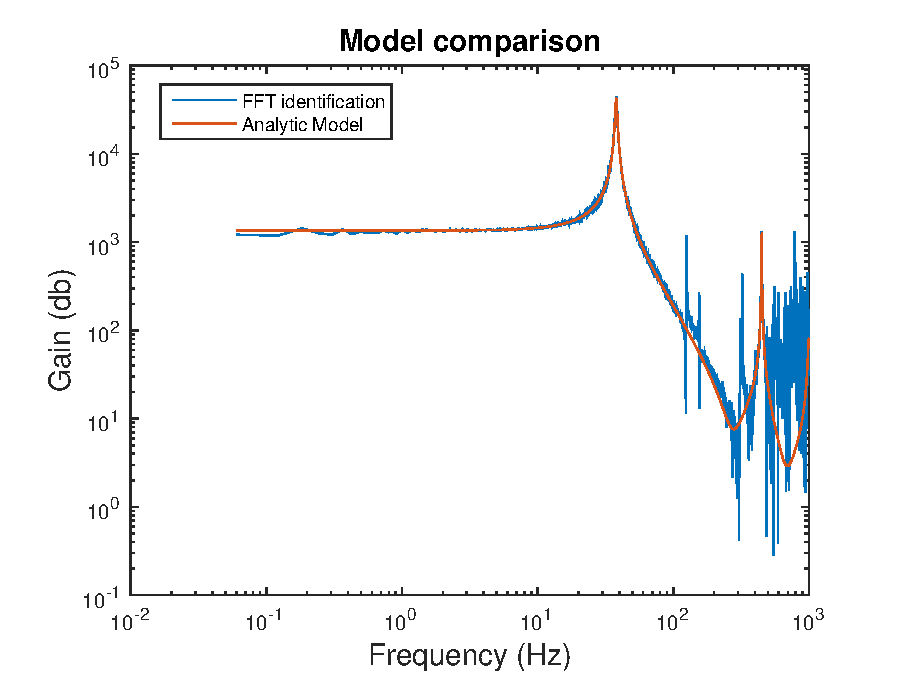
\includegraphics[width=0.7\textwidth]{fig/matlab/model.eps}
  \caption{\label{fig:model} The plot shows the model fit of a transfer function estimation with 5 zeros and 6 poles.}
\end{figure}
The transfer function of the model, discretized with a sampling time of \unit{0.5}{\milli\second}, is presented in \eqref{eq:tf}.

\begin{equation}
  \label{eq:tf}
  G(z) = \frac{21.05z^{-1} - 6.85z^{-2} + 8.52z^{-3} - 0.71z^{-4} + 9.30z^{-5}}{1344 - 2481z^{-1} + 1469z^{-2} + 21.64z^{-3} - 1767z^{-4} + 2084z^{-5} - 639.5z^{-6}}
\end{equation}

\FloatBarrier
\section{Present Control Approach}\label{sec:presentControlApproach}
The original controller for the rotational stage is a 2-\abbrDOF structure (feedback and prefilter). A schematic overview of the control loop is depicted in Figure~\ref{fig:present}, consisting of a controller block C, a prefilter F, a disturbance d and the linearized rotational stage $G = H^{-1}G_0$, where $G_0 = HG$ is the linear and nonlinear dynamics and $H^{-1}$ is the hysteresis compensator.

\begin{figure}[h]
  \centering %crop: left bottom right top
  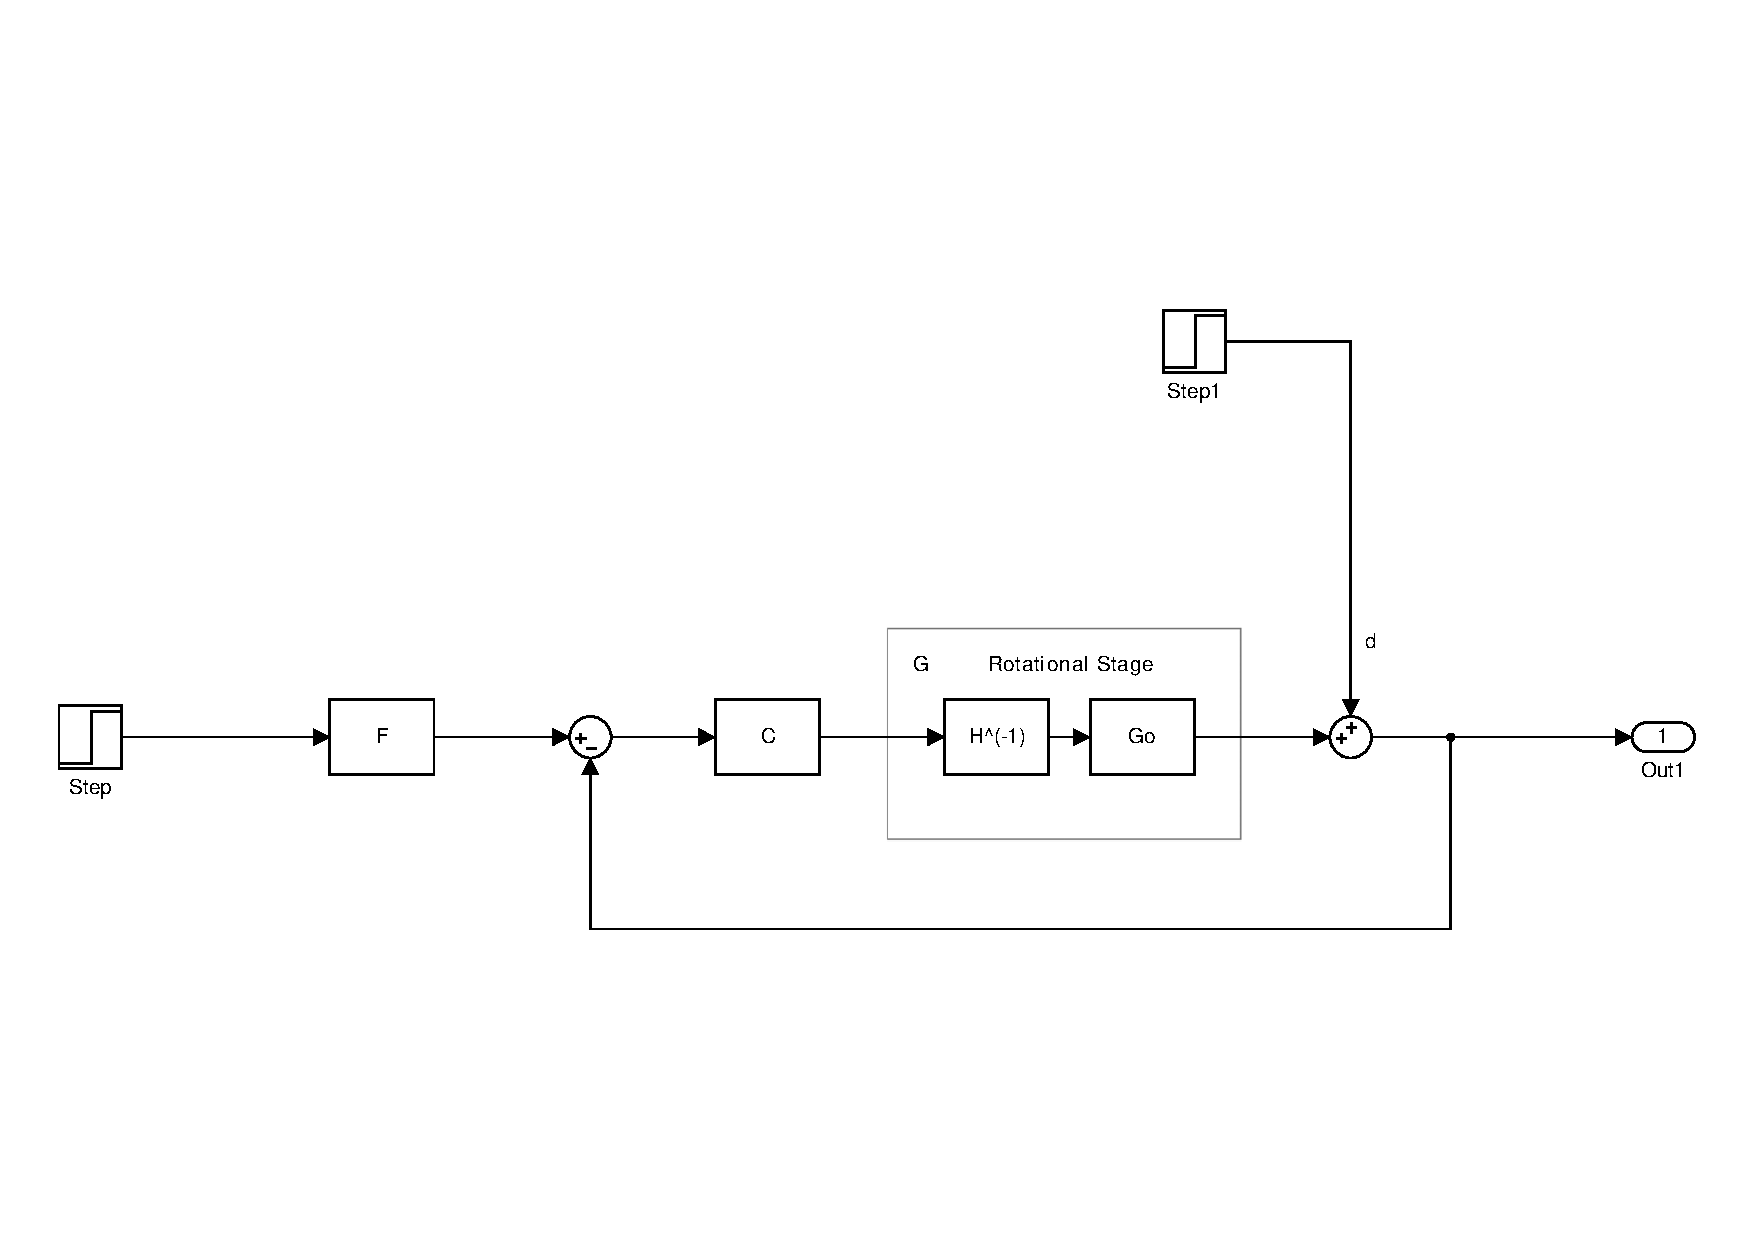
\includegraphics[width=1\textwidth, trim=4cm 3cm 2.1cm 10cm, clip=true]{fig/matlab/present_controller}
  \caption{\label{fig:present}Block diagram of the present control loop, inlcuding controller, prefilter and hysteresis compensator.}
\end{figure}

The controller block (C) is a series combination of a \abbrPID controller, notch filter and a lead filter, aiming to stabilize the system (\abbrPID), increase the sufficient phase margin (lead) and make the system more robust to high frequency oscillations (notch). Since the open loop bandwidth is relatively low, $f_b = 58 Hz$ according to Figure~\ref{fig:model}, it was decided to exclude cancellation of the first resonance peak in order to maintain the bandwidth as high as possible and to have sufficient attenuation of the resonance peak \citep{ButcherController:2015}. Finally, to enhance the tracking performance, a prefilter (F) was also added to the system. The PID controller, lead network, notch filter and prefilter are all presented below in \eqref{eq:controller}.

\begin{subequations}
  \label{eq:controller}
\begin{alignat}{2}
  \label{eq:pre}
  & F = \frac{0.0029z - 0.0029}{z^3 - 2.91z^2 + 2.816 z - 0.91} \\
  \label{eq:pid}
  & C_{PID} = \frac{0.47z^2 - 0.94z + 0.47}{z^2 - 1.78 z + 0.78} \\
  \label{eq:lead}
  & C_{lead} = \frac{4.20 z^2 - 7.72z + 3.55}{z^2 - 1.67z + 0.69} \\
  \label{eq:notch}
  & C_{notch} = \frac{0.28z^4 - 0.62z^3 + 0.75z^2 - 0.59z + 0.26}{z^4 - 1.95z^3 + 1.39z^2 - 0.40z + 0.039}
\end{alignat}
\end{subequations}

The effect of each filter can be seen in Figure~\ref{fig:opensys}, where the open loop system is plotted with one filter added at a time. One can see that the high resonance peak is mitigated after the notch filter have been added, that the lead filter rises the phase and that the \abbrPID controller provides good phase and gain margin. Also the closed loop system is presented in Figure~\ref{fig:closedsys}, proving that the prefilter increases the closed loop bandwidth. The final closed loop bandwidth is 9.7 Hz.

\begin{figure}[h!]
  \centering %crop: left bottom right top
  \subfloat[][\label{fig:opensys} Open loop]{
  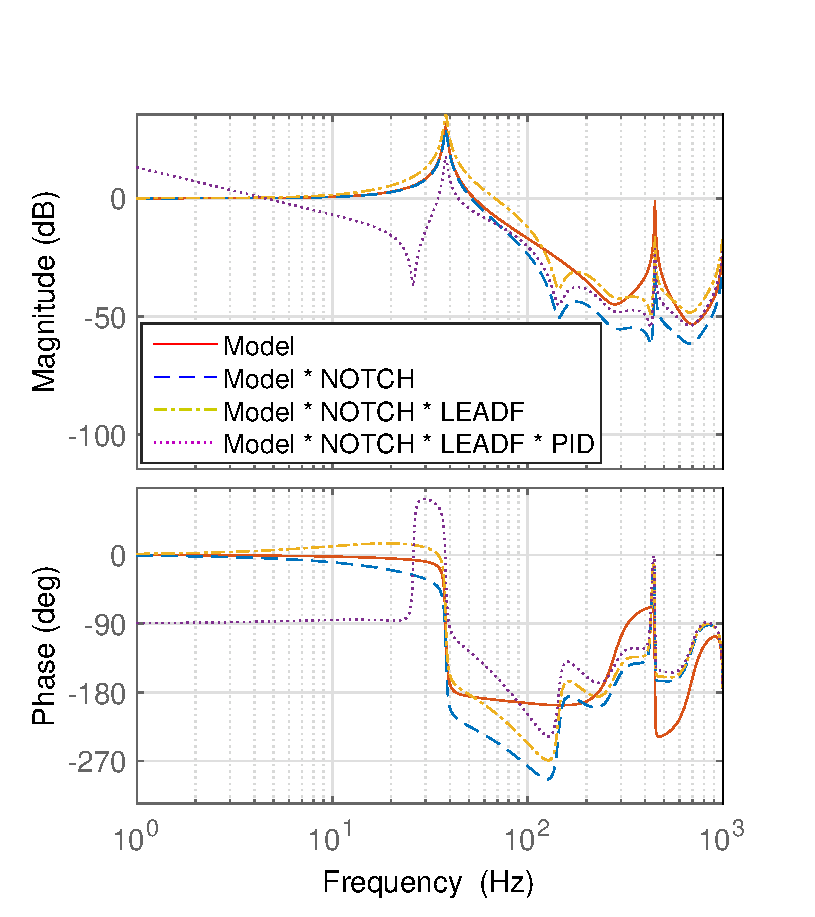
\includegraphics[width=0.46\textwidth, trim=0cm 0cm 1cm 0cm, clip=true]{fig/matlab/openloop_sys.eps}}
  \qquad
  \subfloat[][\label{fig:closedsys} Closed loop]{
  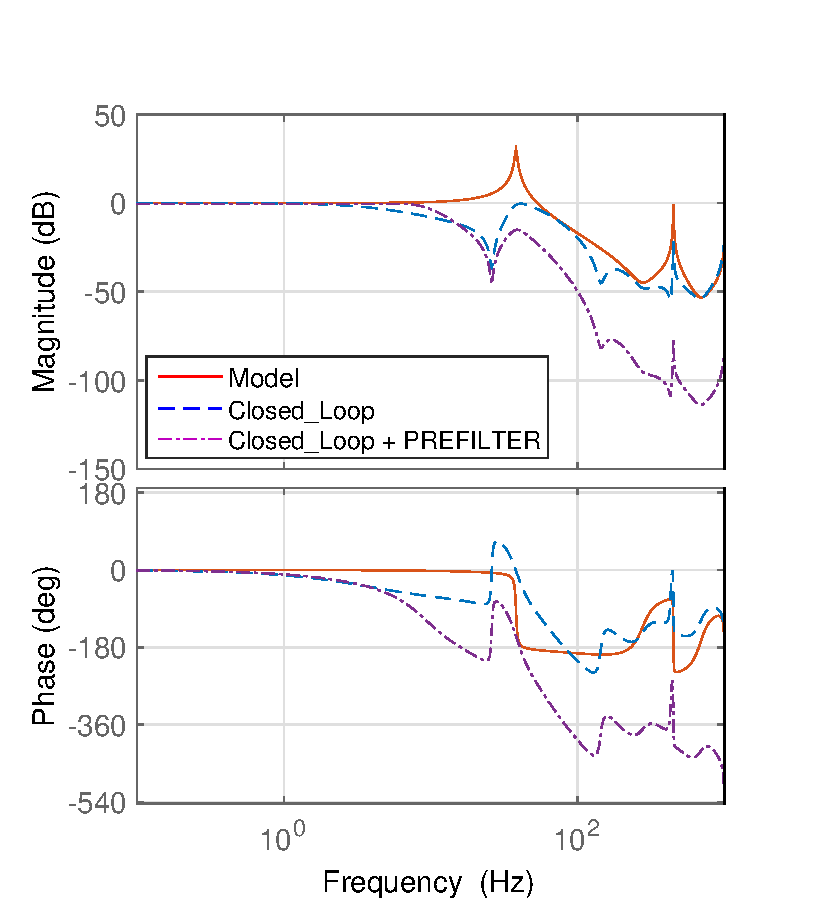
\includegraphics[width=0.46\textwidth, trim=0cm 0cm 1cm 0cm, clip=true]{fig/matlab/closedloop_sys.eps}}
  \caption{\label{fig:open_and_closed_sys} Illustration of controller effect. The effect of adding the different filters is shown in the open loop bode plot in (a) with the resulting closed loop system, with the open loop containing all filters, in (b). }
\end{figure}

% !TEX root = main.tex
\chapter{Theory}\label{cha:modelling}
This chapter presents the motivation and the theory behind each of the control approaches investigated in this thesis.

\section{Model Reference Adaptive Control}
An adaptive controller has the ability to adjust the system response by updating the parameters of a feedback controller in real time, resulting in a controller that is less sensitive to changes in the model and aging of the system. One approach is to use a reference model to create the desired system response which the adaptive laws will aim for, this approach is known as the Model Reference Adaptive Controller (\abbrMRAC). This model does not require any prior knowledge about the model uncertainties, implying in a more straight forward way to implement precision control to nanopositioning systems. Moreover, this scheme allows for the use of a lower order model (in relation to the system model) since the online parameter estimation can be used sufficiently with a lower order model. The \abbrMRAC scheme can be extended to include perturbation estimation (\abbrMRACPE), giving the controller the ability to compensate for various non-modeled effects, including both linear and nonlinear perturbations. Nonlinear effects such as the hysteresis are treated as lumped perturbations to the nominal system model and can be compensated for in the same manner as linear, using the knowledge of the system and the previous measurement and output signal. The \abbrMRACPE also allows the maximum tracking error to be predefined.

\subsection{Perturbation Estimation}\label{sec:pertest}
Using a second order model, the adaptive laws can be derived as follows. Consider the system model stated below.
\begin{equation}
  \label{eq:sysmodel}
  \ddot{x}(t) + \alpha_1\dot{x}(t) +  \alpha_0x(t) = \beta_0u(t) + f(t)
\end{equation}

where $x(t)$ denotes the output rotation at time t, $u(t)$ the input voltage at time t and $\alpha_1, \alpha_0, \beta_0 \in \mathbb{R}$ are known system constants. $f(t)$ is a function describing the unknown perturbations of the system, including the hysteresis and creep effect. The general equations for deriving the perturbation function are described more thoroughly in~\cite{Elmali:1996}, for a simple second order SISO model the perturbation estimation is derived to

\begin{equation}
  \label{eq:perturbation}
  \hat{f}(t) = \ddot{x}_{cal}(t) + \alpha_1\dot{x}_{cal}(t) +  \alpha_0x(t) - \beta_0u(t-T_s)
\end{equation}

where $x_{cal}^{(n)}$ denotes the calculated state, $T_s$ is the sampling time interval and $u(t-T_s)$ is the control input in the previous time step. $u(t-T_s)$ is often approximated to $u(t)$ in practice which is valid approximation if $T_s$ is sufficiently small. Denote that $x(t)$ here is the sensor input, i.e. the measured yaw angle.

Each state is, for its computational efficiency, computed by a simple backward different equation depicted below.

\begin{equation}
  \label{eq:backward}
  x_{cal}^{(n)}(t) = \frac{x_{cal}^{(n-1)}(t) - x_{cal}^{(n-1)}(t-T_s)}{T_s}
\end{equation}

\subsection{Adaptive laws}
The objective of the adaptive laws is to calculate the control parameter so that they converges to ideal values resulting in a system response that matches the reference. The adaptive laws can be derived using Lyaponov theory which is outlined in this section. Consider the second order reference model below

\begin{equation}
  \label{eq:refmodel}
  \ddot{x}_m(t) + a_1\dot{x}_m(t) +  a_0x_m(t) = b_0u_d(t)
\end{equation}

where $x_m(t)$ denotes the output rotation, $u(t)$ the input voltage and $a_0, a_1, b_0$ are known positive constants.

The tracking error is defined as below.
\begin{equation}
  \label{eq:stateerror}
  e(t) = x(t) - x_m(t)
\end{equation}

Recalling~\eqref{eq:sysmodel}, replacing $f(t)$ with the estimation $\hat{f}(t)$ and subtracting it from~\eqref{eq:refmodel} gives the following expression, more details can be found in~\cite{Qingson:2016}.

\begin{equation}
  \ddot{e}(t) + a_1\dot{e}(t) + a_0\dot{e}(t) =  (a_1-\alpha_1)\dot{x}(t) + (a_0-\alpha_0)x(t) - b_0u_d(t) - \beta_0u(t) + \hat{f}(t)
\end{equation}

Transforming it into state-space form
\begin{equation}
  \label{eq:refmodel}
  \mathbf{\dot{E} = AE} + \beta_0\mathbf{B}u + \Delta
\end{equation}
where
\begin{equation}
  \label{eq:matrices}
  \mathbf{E} =
    \begin{bmatrix}
       e\\[0.3em]
       \dot{e}
     \end{bmatrix},
  \mathbf{A} =
    \begin{bmatrix}
       0 & 1\\[0.3em]
       -a_0 & -a_1
     \end{bmatrix},
  \mathbf{B} =
    \begin{bmatrix}
        0\\[0.3em]
        1
    \end{bmatrix},
    \mathbf{\Delta} =
      \begin{bmatrix}
          0\\[0.3em]
          \delta
      \end{bmatrix}
\end{equation}
with $\delta = (a_1-\alpha_1)\dot{x}(t) + (a_0-\alpha_0)x(t) - b_0u_d(t) + \hat{f}(t)$.

If all the eigenvalues of A have negative real parts, then $\mathbf{E}$ will tend to zero as  $t \to \infty$, i.e. the system is asymptotically stable. Moreover, according to Lyaponov theory \cite{Ljung:2003}, for each positive-semidefinite matrix Q, there exist one positive-semidefinite matrix P which solves \eqref{eq:lyap}.

\begin{equation}
  \label{eq:lyap}
  \mathbf{A^TP + PA = -Q}
\end{equation}

With the auxiliary item $\hat{e} = \mathbf{E^TPB}$, the adaptive laws are given by

\begin{equation}
  \label{eq:adaplaws}
  u = k_0u_d + k_1x + k_2\dot{x} + k_3\hat{f}
\end{equation}
where the control law parameters is calculated as
\begin{equation}
  \label{eq:adaplaws1}
  \dot{k}_0 = -\eta_0\hat{e}u_d
\end{equation}
\begin{equation}
  \label{eq:adaplaws2}
  \dot{k}_1 = -\eta_1\hat{e}x
\end{equation}
\begin{equation}
  \label{eq:adaplaws3}
  \dot{k}_2 = -\eta_2\hat{e}\dot{x}
\end{equation}
\begin{equation}
  \label{eq:adaplaws4}
  \dot{k}_3 = -\eta_3\hat{e}\hat{f}
\end{equation}

the proof is provided in \citep{Qingson:2016}. Substituting $\hat{f}$ in \eqref{eq:perturbation} with the one in \eqref{eq:adaplaws} and rearranging the parameters results in the final \abbrMRACPE control law, stated below.

\begin{equation}
    \label{eq:adaplawsfinal}
  u(t) = k_0u_d(t) + (k_1 + k_3\alpha_0)x(t) +  (k_2 + k_3\alpha_1)\dot{x}(t) + k_3\ddot{x}(t) - k_3\beta_0u(t-T_s)
\end{equation}

A block diagram of the final controller, with inspiration from Figure 9.1 in ~\citep{Qingson:2016}, is depicted in Figure~\ref{fig:adaptive}. The adaptive controller consists of 4 blocks. One reference model that calculates the desired states $Xm=[\dot{x}_m, x_m]^T$ from the input signal according to \eqref{eq:refmodel}, one adaptive mechanism that implements \eqref{eq:adaplaws1}-\eqref{eq:adaplaws4} and calculates $K=[k_1, k_2, k_3, k_4]^T$, one state calculator that uses \eqref{eq:backward} to calculate $X=[\ddot{x}, \dot{x}, x]^T$ and finaly one controller block that uses \eqref{eq:adaplawsfinal} to calcuate the control signal $u$ that is sent to the rotational stage.

\begin{figure}[h]
  \centering %crop: left bottom right top
  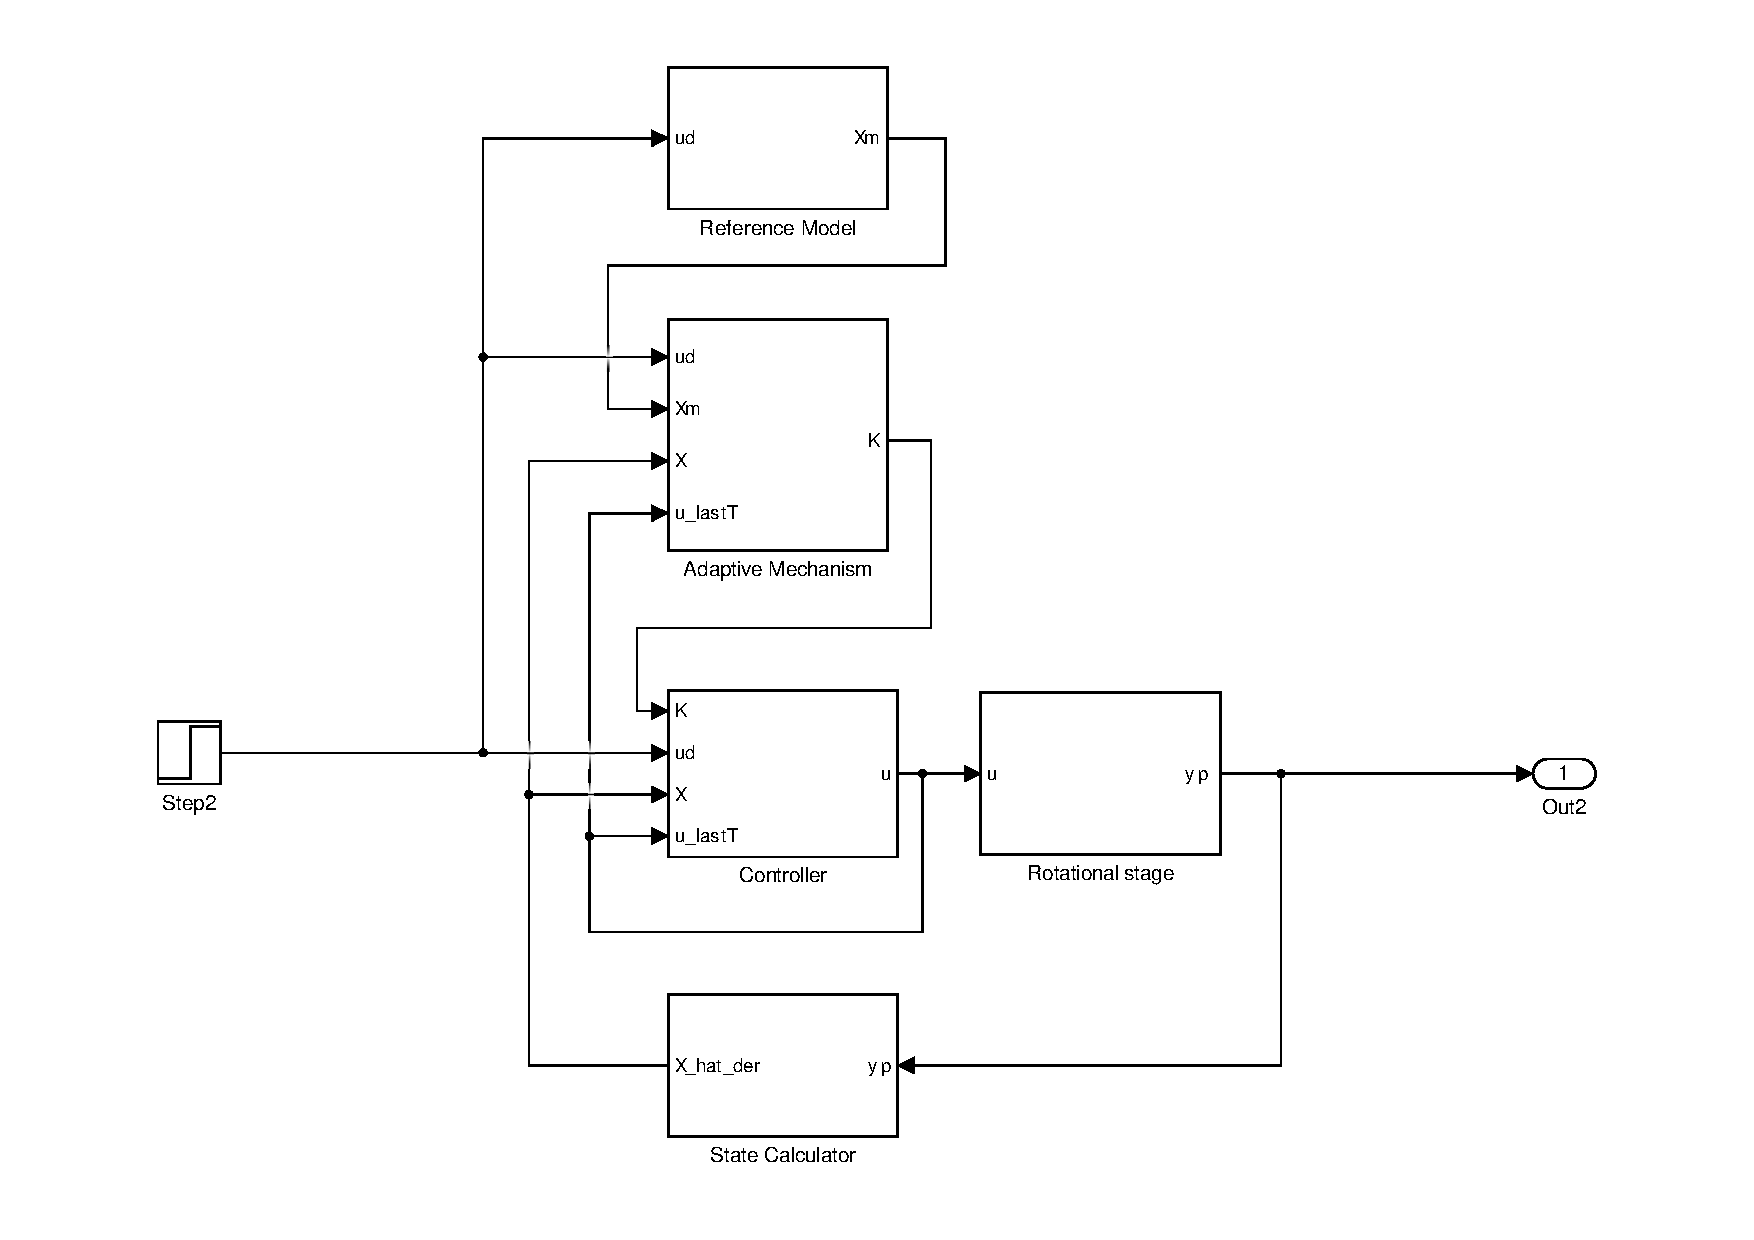
\includegraphics[width=1\textwidth, trim=4cm 0cm 3.8cm 0cm, clip=true]{fig/matlab/adaptive_scheme}
  \caption{\label{fig:adaptive}Block diagram of the adaptive controller}
\end{figure}

\newpage~\newpage~
\FloatBarrier
\section{Integral Resonance Control}\label{sec:irc}
The integral resonace control (IRC) can be efficiently used to damp out the first resonant mode of the system, allowing for larger controller gains and a higher control bandwidth. The \abbrIRC scheme is illustrated in Figure~\ref{fig:irc} and consist of a constant artificial feed-through term $D_f<0$ and an negative integral controller $C=\frac{-k}{s}$ where $k>0$. The negative feed-forward term will, if sufficiently large and negative, introduce a pair of complex zeros below the first resonance frequency and ensure zero-pole cancellation for higher resonance modes as shown in \citep{Aphale:2007}. For stability, the phase response of the loop-gain $CG_d$ must be within $\pm180^{\circ}$ while the gain is greater than 0 dB. The negative sign in $G_d$ subtracts a phase of $-180^{\circ}$. Using this knowledge, the phase margin can easily be increased by applying a simple negative integral controller to provide a 90 degrees phase lead. This results in a phase between $\pm90^{\circ}$ which gives the system highly desired properties such as a $90^{\circ}$ phase margin and an infinite gain margin.

The negative gain $D_f$ is straight forward to manually select for introducing a complex pair of zeros below the first resonance. The integral gain $k$ can be chosen by using the root locus technique and select a gain that maximizes damping.

\begin{figure}[h]
  \centering %crop: left bottom right top
  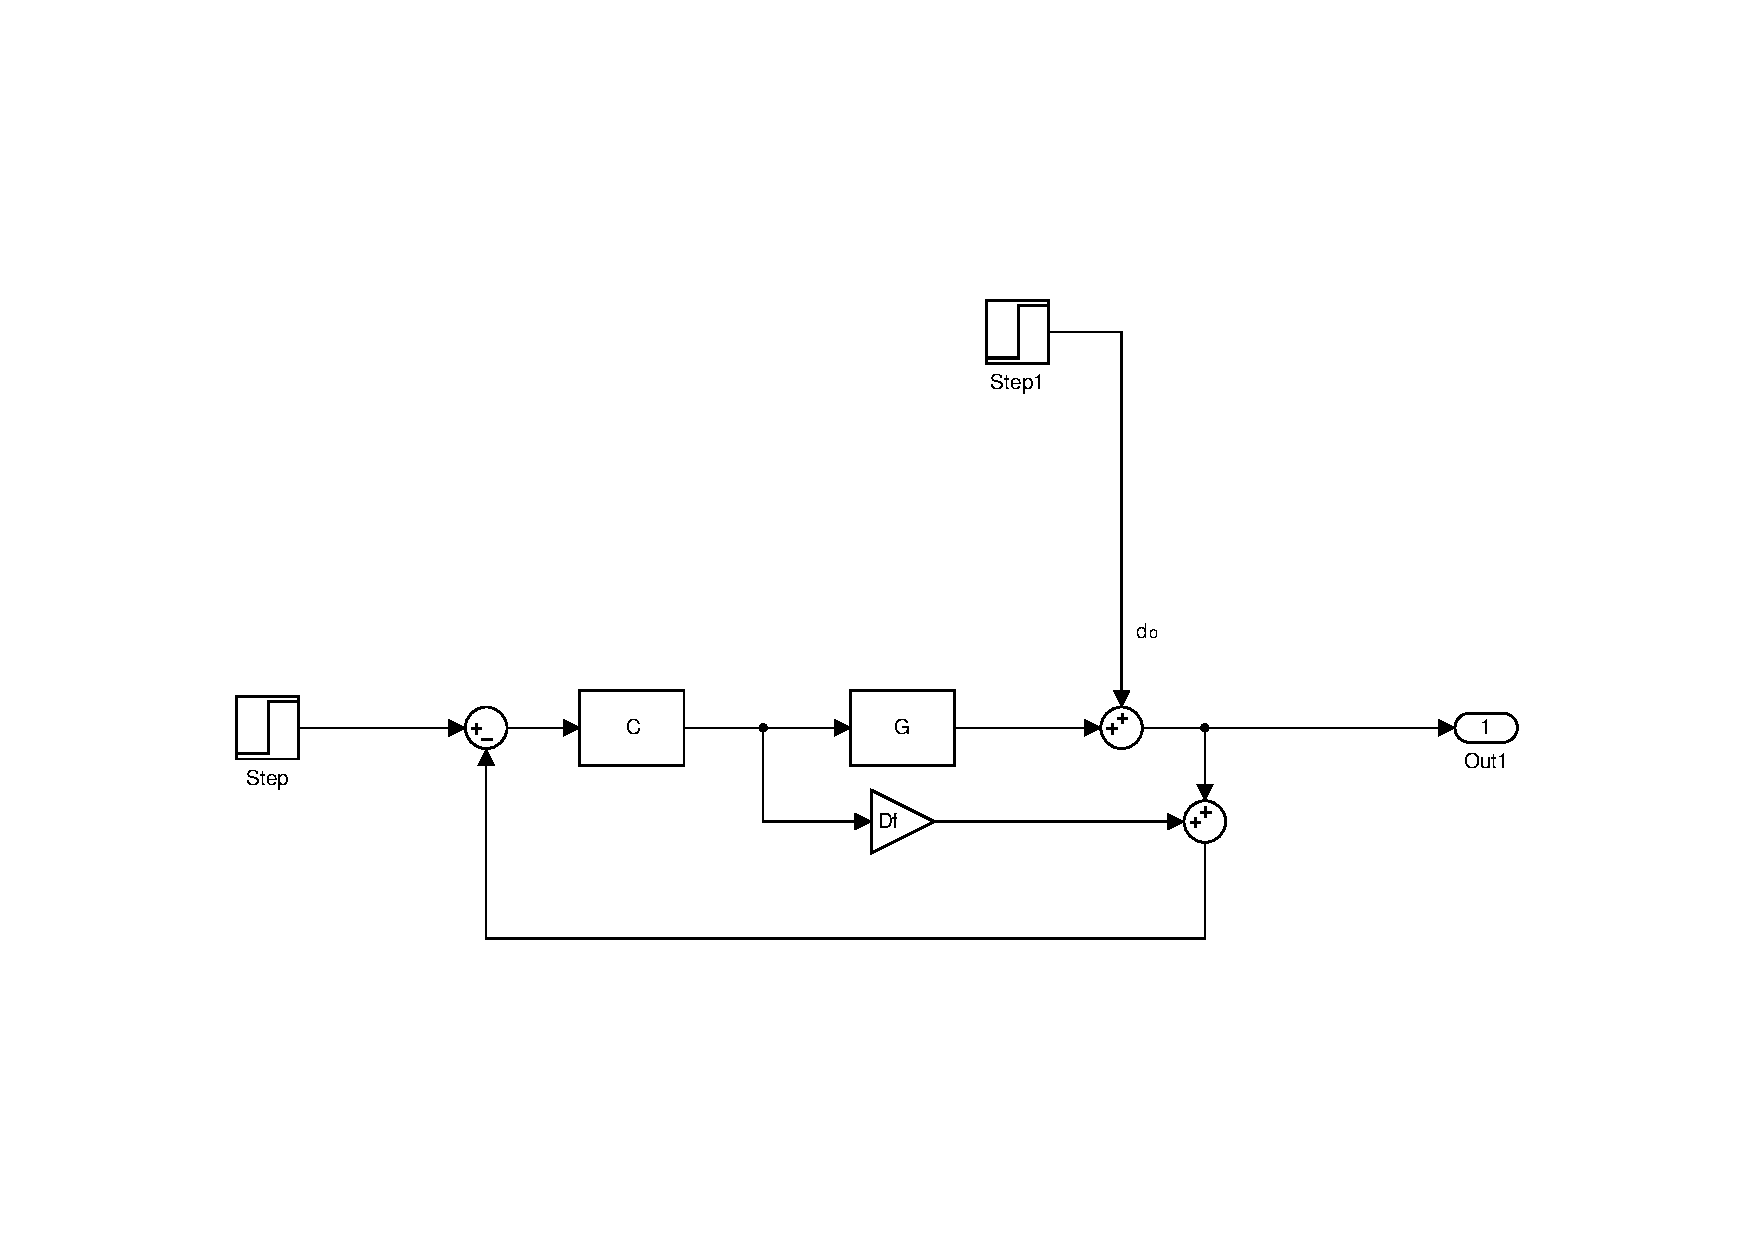
\includegraphics[width=1\textwidth, trim=5.5cm 3cm 5.1cm 9.5cm, clip=true]{fig/matlab/irc}
  \caption{\label{fig:irc}Block diagram of IRC damping loop}
\end{figure}

The IRC scheme in Figure~\ref{fig:irc} can be simplified, by combining $C$ and $D_f$ in the same block, the resulting scheme is shown in the inner loop in Figure~\ref{fig:irc_int}, where

\begin{equation}
  \label{eq:C2}
  C_2 = \frac{C}{1+CD_f}
\end{equation}

For tracking reference trajectories, the IRC can be enclosed in an outer loop, also seen in Figure~\ref{fig:irc_int}, utilizing a second controller $C_1$ to compensate for disturbances and model errors. For the outer controller $C_1$, a PI controller is sufficient but must include a negtive gain to compensate for the inversion that is caused by $D_f$ \citep{gu:2014}.

\begin{figure}[h]
  \centering %crop: left bottom right top
  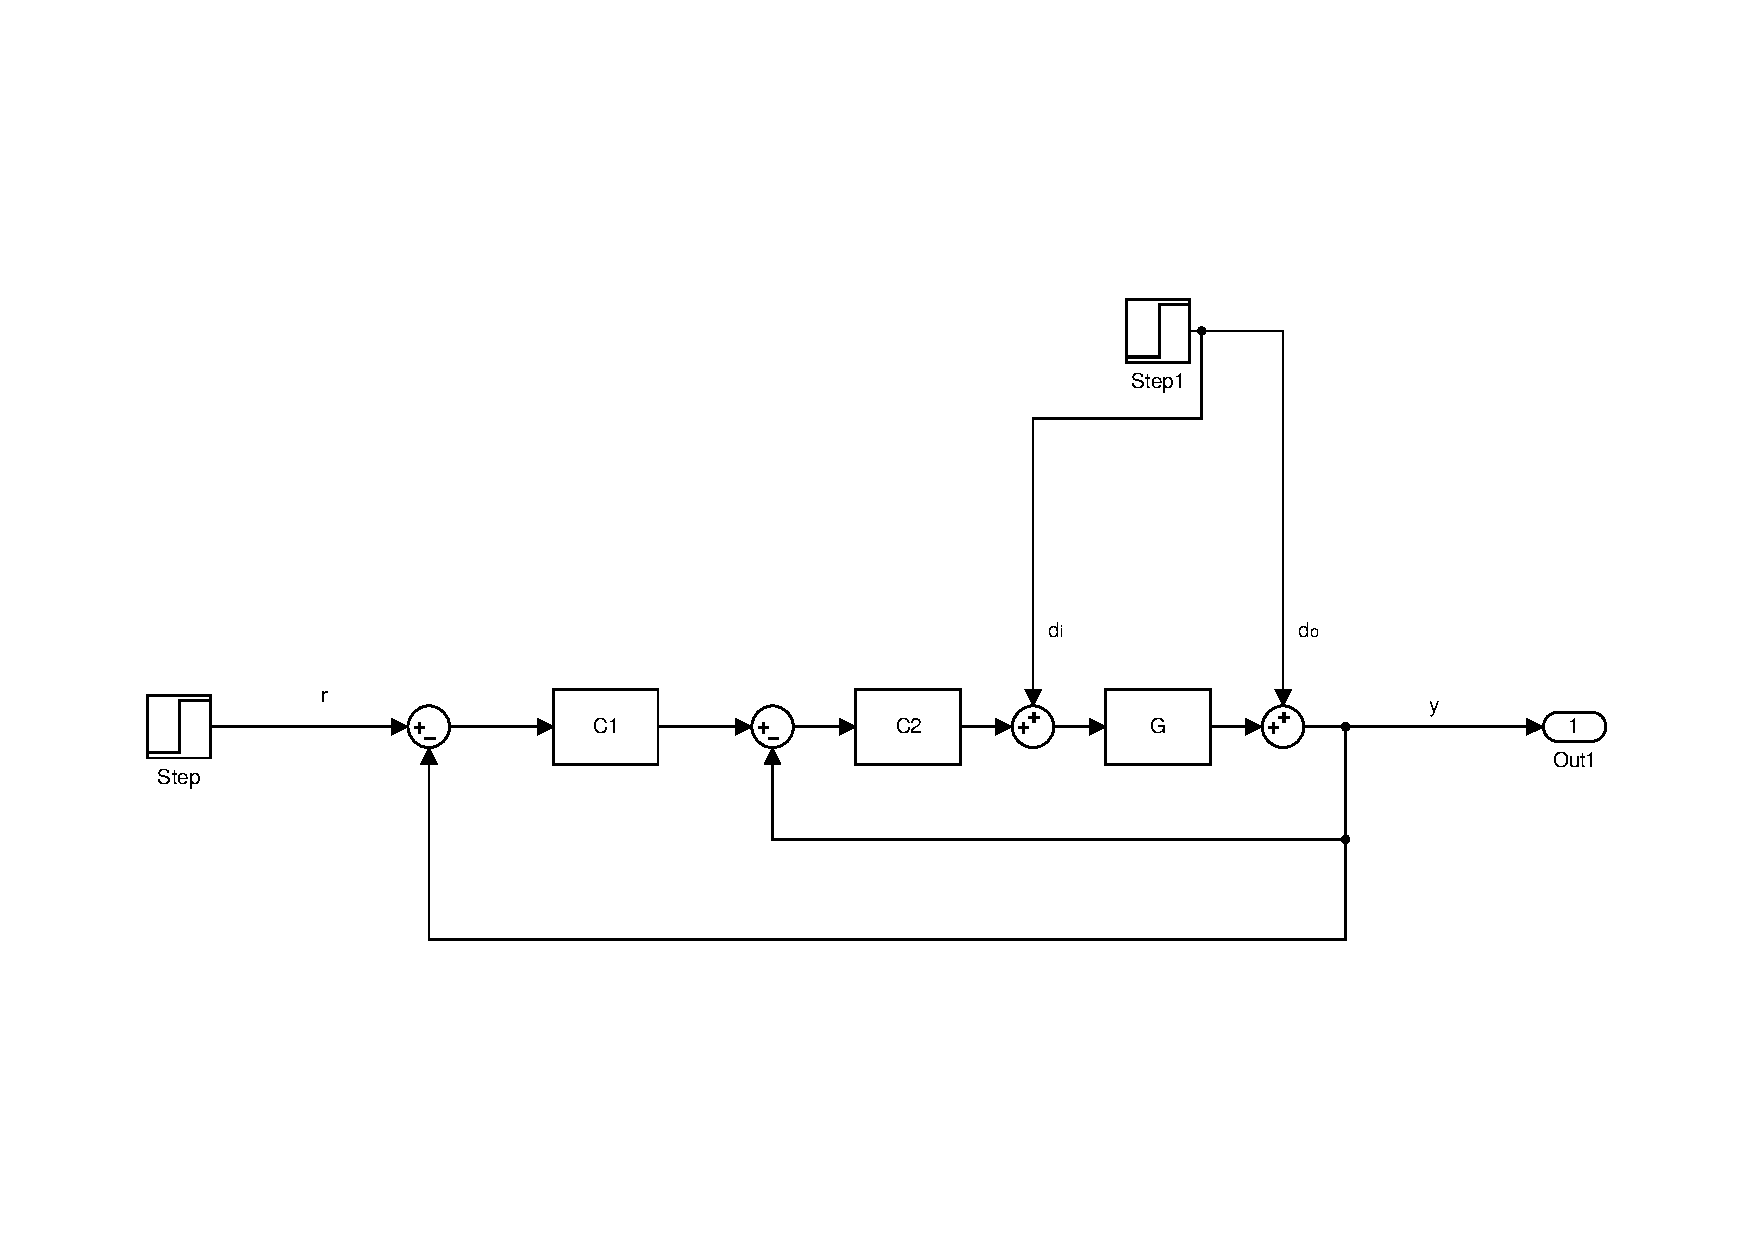
\includegraphics[width=1\textwidth, trim=4cm 5cm 3.6cm 9.5cm, clip=true]{fig/matlab/irc_int}
  \caption{\label{fig:irc_int}Block diagram of the tracking control system with IRC included}
\end{figure}

Proof for the zero-pole interlacement and the insertion of the complex conjugate zeros can be found in \citep{Aphale:2007}, but note that the proof is only given for causal systems with a relative degree of two i.e two more poles than zeros. To give the reader further information about the \abbrIRC and for a system with a relative degree of one, a brief example of a low order system is provided below.

Let G be represented as a transfer function with a relative degree of one, with 2 poles and 1 zero as written below,

\begin{equation}
  \label{eq:irc_sys}
  G = \frac{s + \alpha_0}{s^2 + \beta_1s + \beta_0}
\end{equation}

where  $\alpha_i > 0$ and  $\beta_i > 0$, i.e. a stable and minimum phase system.  Using $G_d = G + D_f$  ~\eqref{eq:irc_sys} and rearranging the terms gives

\begin{equation}
  \label{eq:irc_sys_d}
  \begin{split}
  G_d & = \frac{s + \alpha_0}{s^2 + \beta_1s + \beta_0} + D_f \\
      & = \frac{D_fs^2 + (1 + D_f\beta_1)s + \alpha_0 + D_f\beta_0}{s^2 + \beta_1s + \beta_0} \\
      & = \frac{D_f(s^2 + (\frac{1}{D_f} + \beta_1)s + \frac{\alpha_0}{D_f} + \beta_0)}{s^2 + \beta_1s + \beta_0}
  \end{split}
\end{equation}

which illustrates that the number of introduced zeros is equal to the relative degree of the transfer function and that the zeros ($s^z_i$) will have a negative real part if the following conditions are fulfilled.

\begin{equation}
  \label{eq:irc_cond}
  Re(s^z_i) < 0 \quad \text{if }
  \begin{cases}
    D_f < -\frac{1}{\beta_1}\\
    D_f < -\frac{\alpha_0}{\beta_0}\\
  \end{cases}
\end{equation}

\section{Harmonic cancellation}
Cancellation of specific harmonics can be utilized to increase the tracking capability of a controller. A known or estimated disturbance can in many cases be efficiently eliminated by a number of methods \citep{fujimoto2009rro} \citep{fujimoto2004repetitive} \citep{vilanova2008disturbance}. Many of these approaches are based on the Internal Model Principle (\abbrIMP) meaning that the controller incorporates a known model of the disturbance within the control loop itself. However including the disturbance model for effective cancellation in the feedback loop will deteriorate the sensitivity function making the system more sensitive to other frequencies. Hence, a feedforward approach is preferable to preserve the fine closed loop characteristics. This approach aims to cancel the periodic disturbances that are introduced by the movement of the linear stage. The period lengths of the introduced harmonics can be found  from characterizing tests and should correlate with the stepping rate of the linear axis motor. For the sake of completeness, the \abbrIMP feedback approach is included in this chapter and evaluated in simulations to verify the expected results.

\subsection{Feedforward Disturbance Cancellation}\label{subsec:distff}
If a disturbance is measurable during operation, a feedforward of the disturbance model response can be used to eliminate the disturbance before it gets present in the output signal \citep{industrial}. A simple block diagram of the structure is shown in Figure~\ref{fig:ffdist}, where $G, C, P_d$ and $K_f$ represents the system, the controller, the disturbance model and the feedforward block respectively.

\begin{figure}[h]
  \centering %crop: left bottom right top
  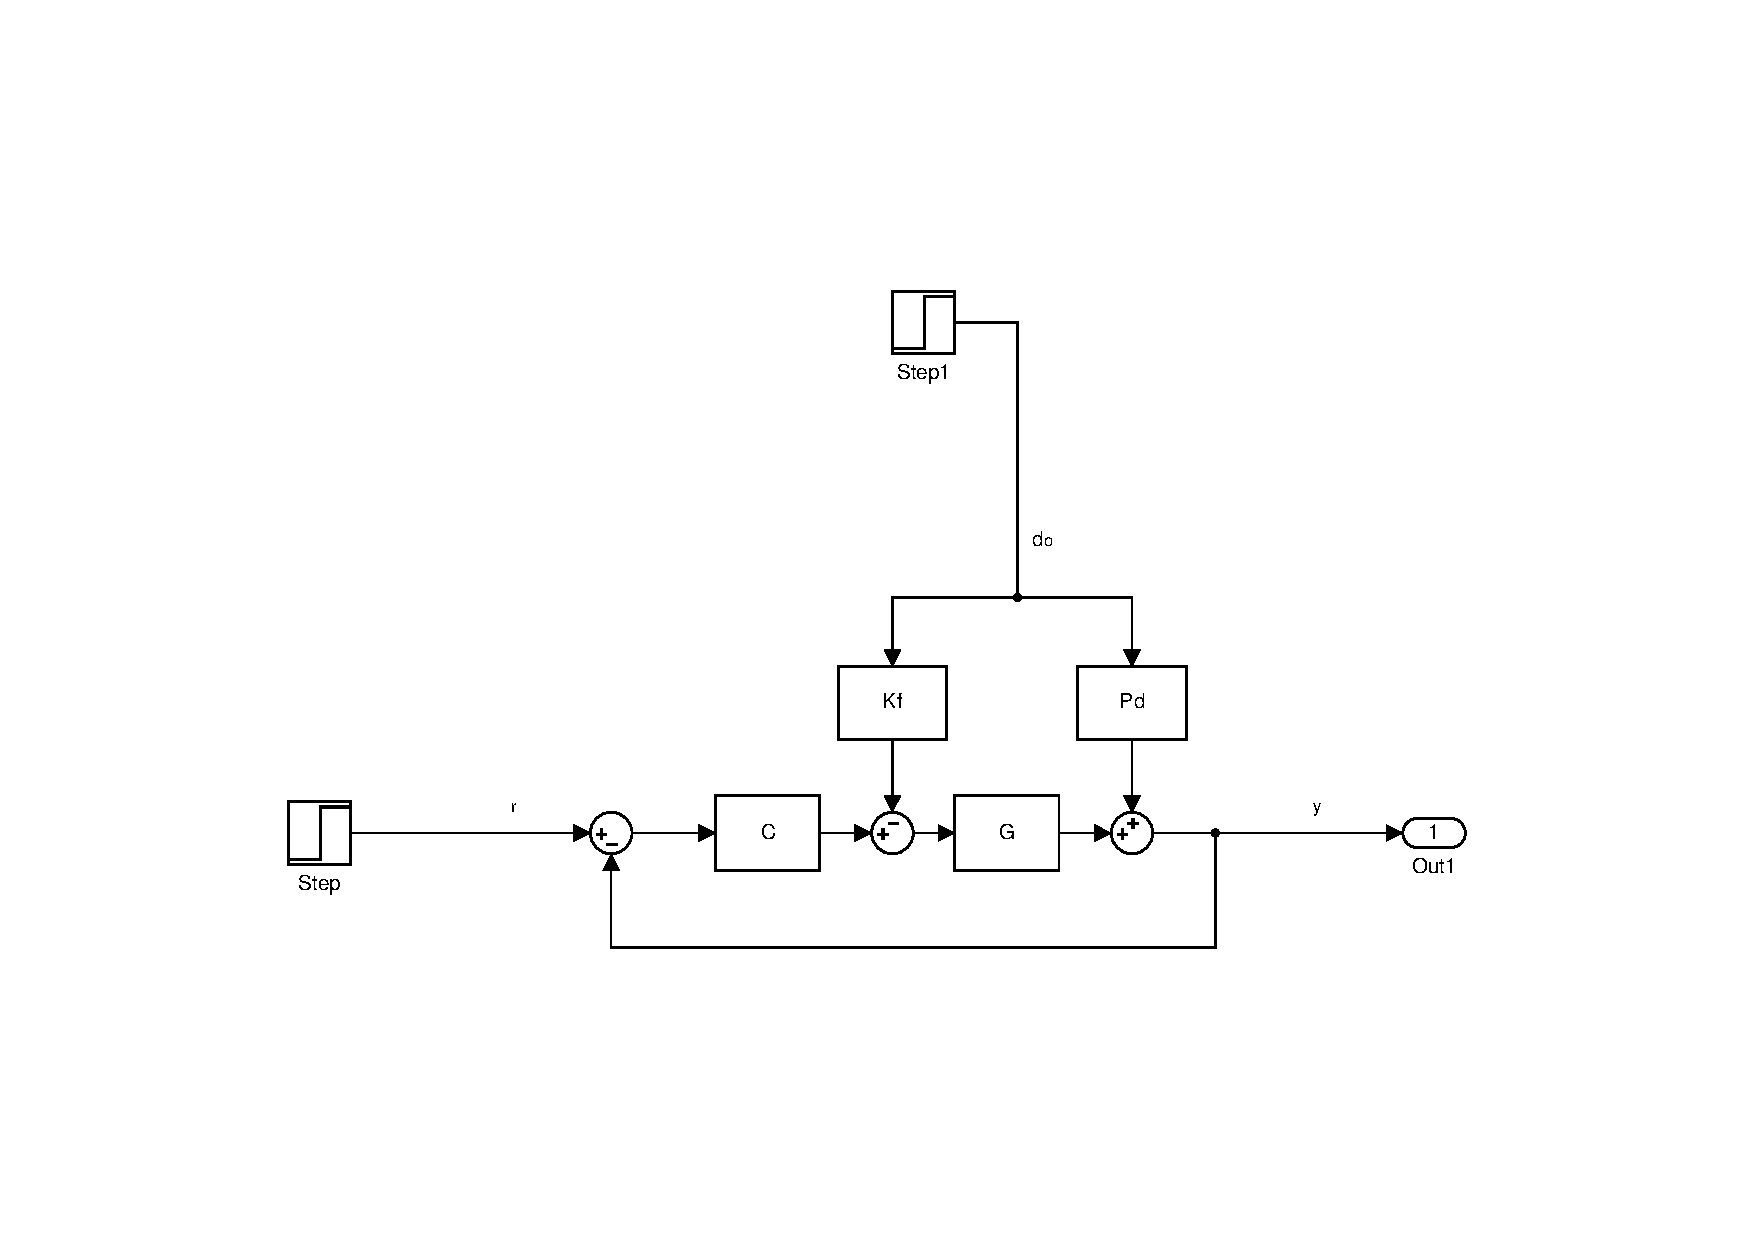
\includegraphics[width=0.8\textwidth, trim=8cm 4.5cm 5.97cm 8.5cm, clip=true]{fig/matlab/ffdist}
  \caption{\label{fig:ffdist}Block diagram of a control structure with feedforward from a known modeled disturbance.}
\end{figure}

The output is described by the following expression

\begin{equation}
  \label{eq:ffdist}
  Y = \frac{CG}{1+CG}R + \frac{P_d - K_fG}{1+CG}D_0
\end{equation}

and hence a ideal choice of $K_f$ would be $K_f=P_d/G$ which would eliminate the disturbance completely. It is worth noting that the ideal $K_f$ might not be fully implementable (stable, proper and causal) and that the inverse of G has to be approximated, leading to merely partial cancellation of the disturbance. This approximation can still be sufficient if the inverse is constructed in a way so that $(P_d - K_fG)/(1+CG)$ becomes small for the frequencies where the disturbance has the most impact on the system.

\subsection{Cancellation with Internal Model Principle}\label{subsec:distimp}
The \abbrIMP says that if a disturbance (entering the system on the output or input) can be described by a generating polynomial $\Gamma(s)$ then a standard one \abbrDOF-controller $C_{t}(s) = P(s)/\Gamma(s)\bar{L}(s)$ can be used to asymptotically reject the effect of a modeled disturbance.  The generating polynomial $\Gamma(s) = f(0,s)/D(s)$, is derived by taking the Laplace transform of the differential equation describing the disturbance where f(0,s) arises from non-zero initial conditions. To show the principle of \abbrIMP parts of the evidence derived in \citep{IMP:Perry} is presented here.

Consider the system model $G(s) = A(s)/B(s)$. Using this system with the controller $C_t$ in closed loop yields the sensitivity function in \eqref{eq:s_imp}, which is the transfer function from output disturbance to output.
\begin{equation}
  \label{eq:s_imp}
  S(s) = \frac{A(s)\Gamma(s)\bar{L}(s)}{A(s)\Gamma(s)\bar{L}(s) + B(s)P(s)}
\end{equation}

The system response to an output disturbance can then be derived as shown in \eqref{eq:s_imp}.

\begin{equation}
  \label{eq:y_imp}
  Y(s) = S(s)D_o(s) = \frac{S(s)f(o,s)}{\Gamma(s)} = \frac{A(s)\bar{L}(s)}{A(s)\Gamma(s)\bar{L}(s) + B(s)P(s)}f(o,s)
\end{equation}

The inverse Laplace transform y(t) converges to 0 if the controller has been tuned so that all roots to the characteristic polynomial $A(s)\Gamma(s)\bar{L}(s) + B(s)P(s)$ have negative real parts. Hence, the disturbance is asymptotically rejected.

A basic block scheme is shown in Figure~\ref{fig:imp} where $G$ is the system, $C(s) = P(s)/\bar{L}(s)$ the tunable controller, $C_{imp} = 1/\Gamma(s)$ is the compensator and $d_o$ is the considered disturbance.

\begin{figure}[h]
  \centering %crop: left bottom right top
  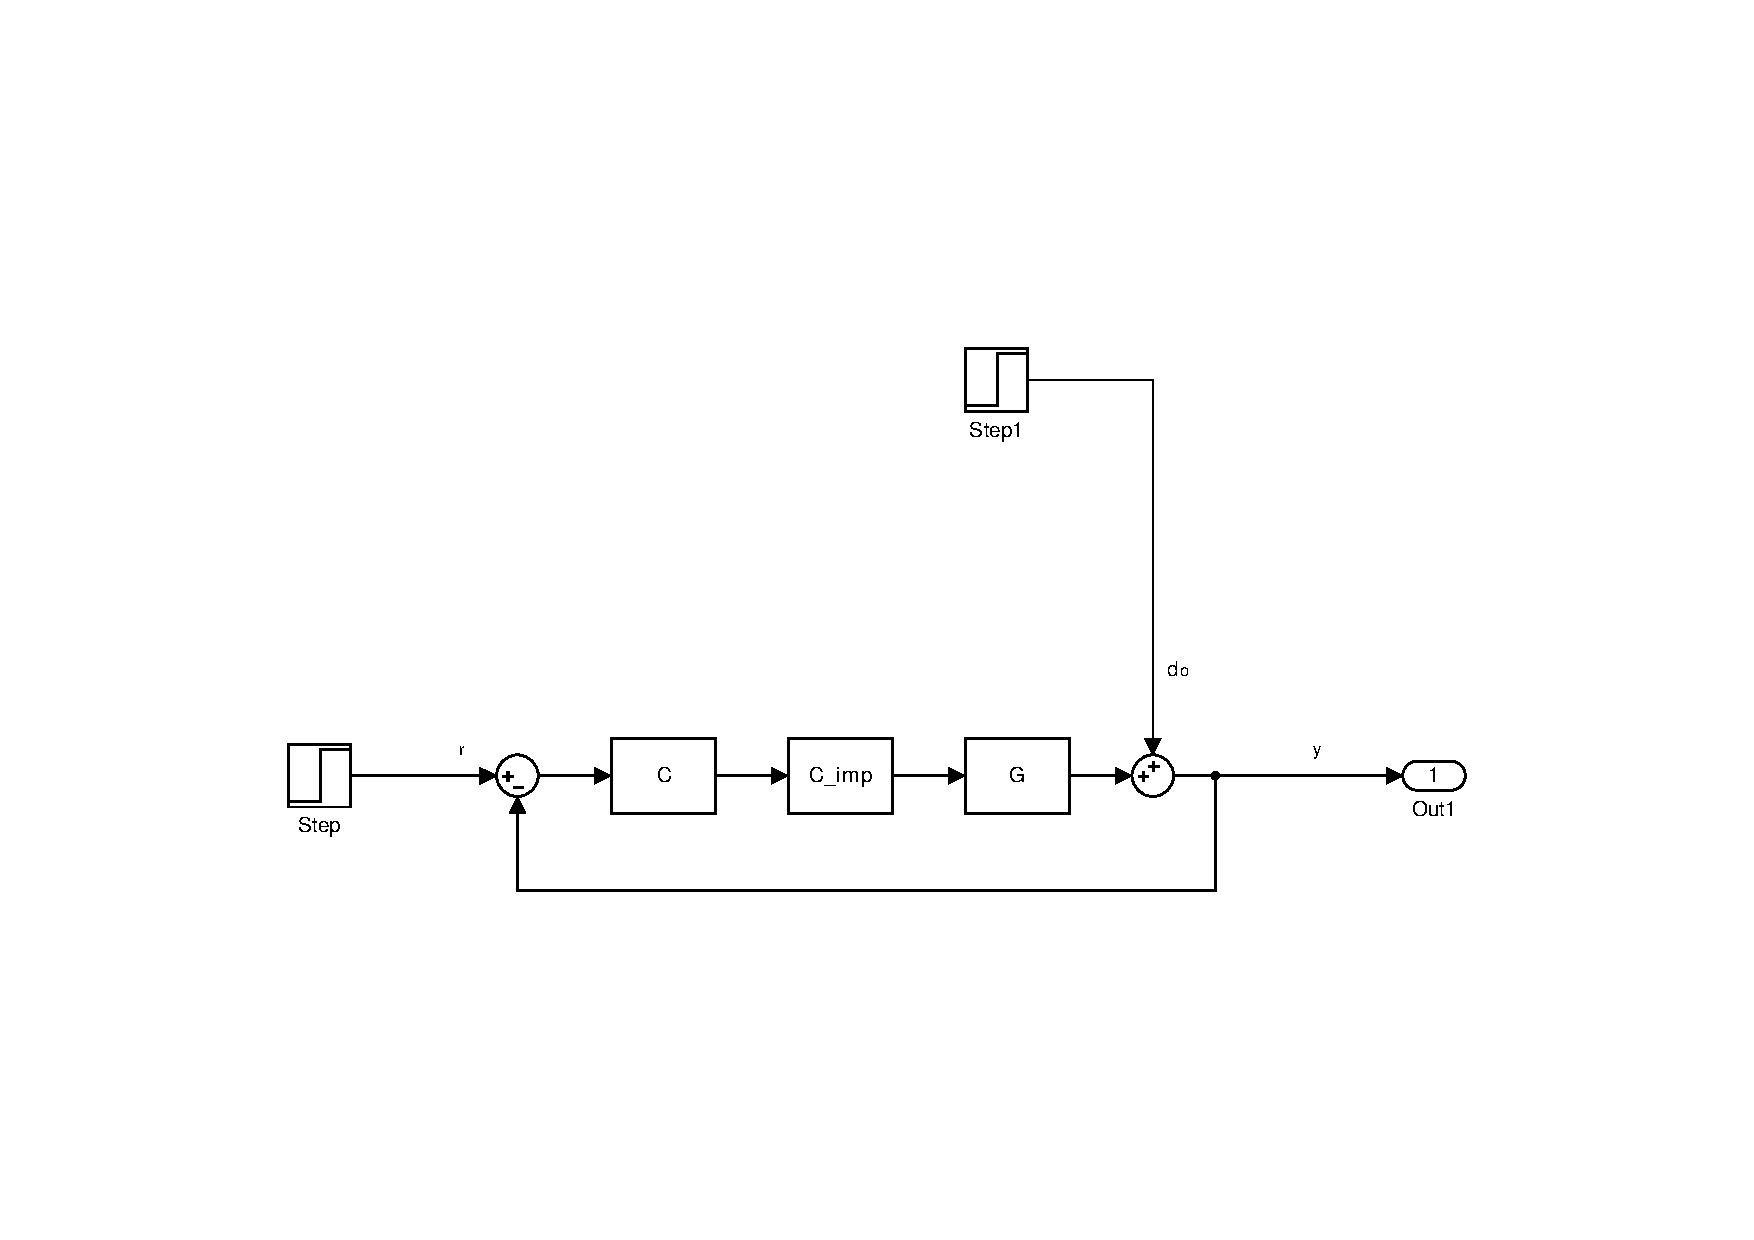
\includegraphics[width=1\textwidth, trim=6.5cm 5.5cm 5.97cm 11cm, clip=true]{fig/matlab/imp}
  \caption{\label{fig:imp}Block diagram of the \abbrIMP control structure.}
\end{figure}

\subsection{Repetitive Feedforward Disturbance Cancellation}
Repetitive control can sufficiently be used to track and reject periodic disturbances with relatively long periods. For higher frequency modes, it fails to do so due to a number of reasons but mostly for the inclusion of a low-pass filter which is needed to maintain stability \citep{fujimoto2009rro}. The conventional repetitive approach uses the \abbrIMP to include a discrete time disturbance model in the feedback controller. Although the sensitivity function is zero for the selected frequencies, it is increased for the other nearby frequencies, leading to severe damage in the total tracking accuracy. This phenomenon can be explained by Bode's integral constraints \citep{Ljung:2003}. With respect to this drawback, a novel control scheme with a feedforward switching mechanism and an observer was introduced by the authors in \citep{fujimoto2004repetitive}, for the purpose of head-tracking control in hard disk drives. A block scheme of the novel control scheme is presented in Figure~\ref{fig:ffrep}, where $G$ and $C$ represents the system and the feedback controller as before. The output disturbance and the observed and replicated compensation signal are denoted $d_o$ and $d_i$, respectively.

\begin{figure}[h]
  \centering %crop: left bottom right top
  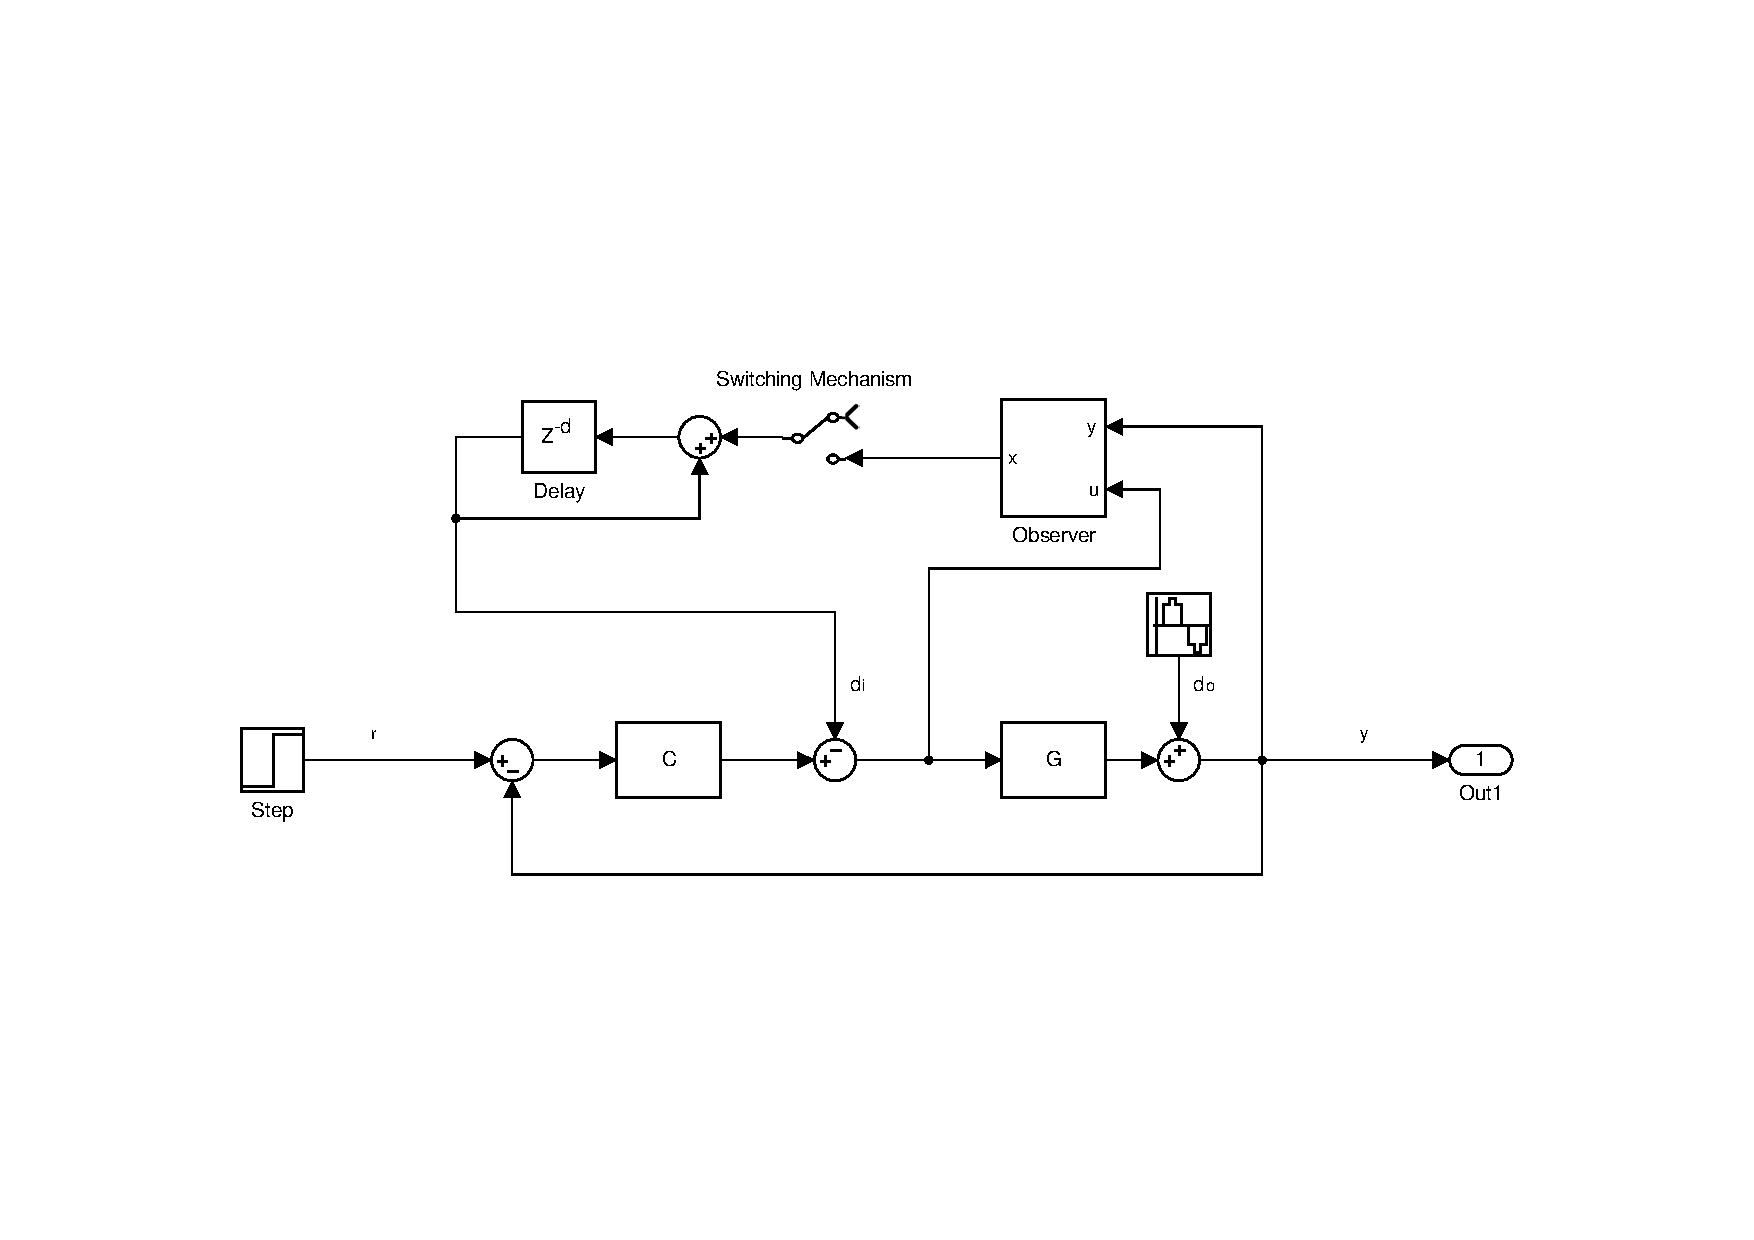
\includegraphics[width=1\textwidth, trim=6cm 5.5cm 5.2cm 5.5cm, clip=true]{fig/matlab/ffrep}
  \caption{\label{fig:ffrep}Block diagram of the feedforward switching mechanism including observer and feedback controller.}
\end{figure}

This method uses an observer to estimate the states of the disturbance. When the states have converged the switch is turned on for one period $T_d$ of the disturbance. This period is then replicated and used to subtract the disturbance from the input signal as illustrated in the block diagram. The delay constant $d$ and the switching on and off time have to be set in advance, hence $T_d$ must be known. Note that if the disturbance frequency is not a multiple of the sampling frequency $T_s$ then extra care has to be taken when setting the delay and switching times. Multiple periods should preferably be used to get a full number of oscillations within the switching timespan that is switched with a period of $T_s$.

The continues time system in \citep{fujimoto2004repetitive} is defined with $d_o$ added on the input. External disturbances are better modeled as disturbances added to the system output, therefore this approach has changed the position of $d_o$. However, the observer should still be modeling $d_o$ as if it would be added to the input, see \eqref{eq:sys1}, to maintain cancellation of the harmonics at the input of the system. This assumes that $G$ is linear and that the disturbance is sufficiently described by a sinusoidal, since a sinusoidal added as input to a linear system only results in a change in phase and magnitude of the input sinusoidal.

Using a continues time state space representation the system and the disturbance can be described as follows

\begin{subequations}
  \label{eq:sys12}
  \begin{alignat}{2}
    \label{eq:sys1}
    & \mathbf{\dot{x}}(t) = \mathbf{A_cx}(t) + \mathbf{B_c}(u(t) + d_o(t)) \\
    \label{eq:sys2}
    & y(t) = \mathbf{C_cx}(t)
  \end{alignat}
\end{subequations}

and the disturbance as

\begin{subequations}
  \label{eq:dist12}
  \begin{alignat}{2}
    \label{eq:dist1}
    & \mathbf{\dot{x}}_d(t) = \mathbf{A_dx_d}(t) \\
    \label{eq:dist2}
    & d_o(t) = \mathbf{C_dx_d}(t)
  \end{alignat}
\end{subequations}

where $\mathbf{x}$ and $\mathbf{x_d}$ is the system and disturbance state vector and $\mathbf{A_c, B_c, A_d, C_c}$ and $\mathbf{C_d}$ are known system and disturbance matrices. The Laplace transform of $\frac{1}{w}sin(wt)$ is $1/(s^2 + w^2)$, yielding the state space equations in \eqref{eq:sinm} with zero input.

\begin{equation}
  \label{eq:sinm}
  \mathbf{A_d} =
    \begin{bmatrix}
       0 & 1\\[0.3em]
       -w^2 & 0
     \end{bmatrix}
     \qquad
  \mathbf{C_d} =
    \begin{bmatrix}
        1 & 0\\
    \end{bmatrix}
\end{equation}

The discrete state space representations are obtain by using \eqref{eq:discr123} from \citep{industrial}

\begin{equation}
  \label{eq:discr123}
  A_z = e^{AT_s}  \qquad B_z = \int_{0}^{Ts} e^{AT_s}B dt \qquad C_z = C
\end{equation}

yielding the equations in \eqref{eq:discrsys}

\begin{subequations}
  \label{eq:discrsys}
  \begin{alignat}{2}
    & \mathbf{x_{zs}}[n + 1] = \mathbf{A_{zs}x_{zs}}[n] + \mathbf{B_{zs}}(u_z[n] + d_{zo}[n]) \\
    & y_{zs}[n] = \mathbf{C_{zs}x_{zs}}[n] \\
    & \mathbf{x_{zd}}[n + 1] = \mathbf{A_{zd}x_{zd}}[n]\\
    & d_{zo}[n] = \mathbf{C_{zd}x_{zd}}[n]
  \end{alignat}
\end{subequations}

where the disturbance and input are assumed to be piecewise constant during each sampling period $T_s$.

The disturbance is estimated by an observer which is given as

\begin{equation}
  \label{eq:obs}
  \mathbf{\hat{x}}[n + 1] = \mathbf{A\hat{x}}[n] + \mathbf{B}u[n] + \mathbf{K}(y[n] - \mathbf{C\hat{x}}[n])
\end{equation}

where $\mathbf{A, B}$ and $\mathbf{C}$ are the augmented system matrices and $\mathbf{K}$ is the observer gain.

\begin{equation}
  \label{eq:augumented}
  \mathbf{A} =
    \begin{bmatrix}
       \mathbf{A_{zs}} & \mathbf{C_{zd}B_{zs}}\\[0.3em]
       \mathbf{0} & \mathbf{A_{zd}}\\
     \end{bmatrix}
     \qquad
  \mathbf{B} =
    \begin{bmatrix}
        \mathbf{B_{zs}}\\
        \mathbf{0}
    \end{bmatrix}
     \qquad
  \mathbf{C} =
    \begin{bmatrix}
        \mathbf{C_{zs}} & \mathbf{0}\\
    \end{bmatrix}
\end{equation}

The observer gain should be tuned (placing the eigenvalues of $\mathbf{A-KC}$) with respect to the tradeoff between the quickness in the state reconstruction and the sensitivity to measurement noise. An optimal choice of K can be calculated by the Kalman filter if the noise intensities are known. By deriving the closed loop system, it is shown in \citep{fujimoto2004repetitive} that the disturbance rejection will be achieved at every sampling point in steady state.

The method can be extended to estimate and reject $n$ harmonics by extending $\mathbf{A_d}$ as shown in \eqref{eq:sinexten}, adding $n$ delay loops for each estimated disturbance and by  summing all replicated disturbances i.e. $d_i = \sum_{k=1}^{n} d_k$.

\begin{equation}
  \label{eq:sinexten}
  \mathbf{A_{de}} =
    diag(\begin{bmatrix}
      \mathbf{A_{d1}}  &  \mathbf{A_{d2}} & \hdots & \mathbf{A_{dn}} \\
     \end{bmatrix})
     \qquad
  \mathbf{C_{de}} =
    \begin{bmatrix}
       \mathbf{C_{d1}}  &  \mathbf{C_{d2}} & \hdots & \mathbf{C_{dn}} \\
    \end{bmatrix}
\end{equation}

%\begin{chapter-appendix}
%  \label{ap:lyaponov}

%\section{MRACPE}

%\end{chapter-appendix}

% !TEX root = main.tex
\chapter{Simulation Results}\label{cha:result}
This section describes the simulation results considering performance, robustness and stability with respect to the different control approaches. All approaches will first be benchmarked with the present control approach and presented individually in the following subsections. A comparison table outlining the performance and the robustness of each controller will be presented in the end of this chapter.

\section{Benchmark Tests}
For the comparison with the present control approach, all evaluated controllers were discretized with a sampling frequency of 2kHz. The normalized system in \eqref{eq:tf} was used to model the rotational stage linear dynamics. The nonlinear dynamics, creep and hysteresis, were neglected in the simulations, assuming perfect inverse hysteresis cancellation and a sufficient closed loop to compensate for the creep effect. All simulations were performed in Matlab and in combination with Simulink. Each of the control approaches has been evaluated with respect to robustness to model errors, disturbance rejection, closed loop bandwidth and response to step and periodical input, all listed below.

\begin{itemize}
\item {\bf Step, ramp and periodical tracking} - A step and a periodical input is applied to the input to benchmark the tracking capability of the controller.
\item {\bf Disturbance rejection} - Modified step responses with impulses added to the input and measurement signal to benchmark how sensitive the system is to system disturbances.
\item {\bf Robustness to model errors} - The robustness to model errors is characterized by changing the dynamical model, either during runtime or instantaneously.
\end{itemize}

 The prospective challenges, described in \ref{sec:prospectiveChallanges} shall be kept in mind while reading the results. Since the required ramp rates are relatively low, the disturbance rejection and the robustness to model errors are more of interest when evaluating each method.

\section{Linear Dynamics Characterization}
The linear dynamics of the rotational stage changes due to the a number of physical properties of the system, such as the current yaw-position, the linear axis position and speed and if the system is in contact with the end-switches. This phenomenas were characterized in a number of tests and summarized below. Figure~\ref{fig:different_angles} shows a comparison of the identified model when the linear axis is in its outer position and the rotational head has rotated 0 mrad (0V), 10 mrad (3.25V) and 20 mrad (6.5V). It shows that the system changes its first resonance peak as much as 15.3 Hz.

Figure~\ref{fig:different_lin_pos} shows a comparison of the identified model when the rotational head is in 10 mrad (3.25V) and the linear axis position is in 1, 20, 40 and 57mm. The identified system are almost the same for the first 3 positions, but it changes drastically when the linear axis touches the outer switches in 57mm.

\begin{figure}[h!]
  \centering %crop: left bottom right top
  \subfloat[][\label{fig:different_angles}Different rotational head positions]{
  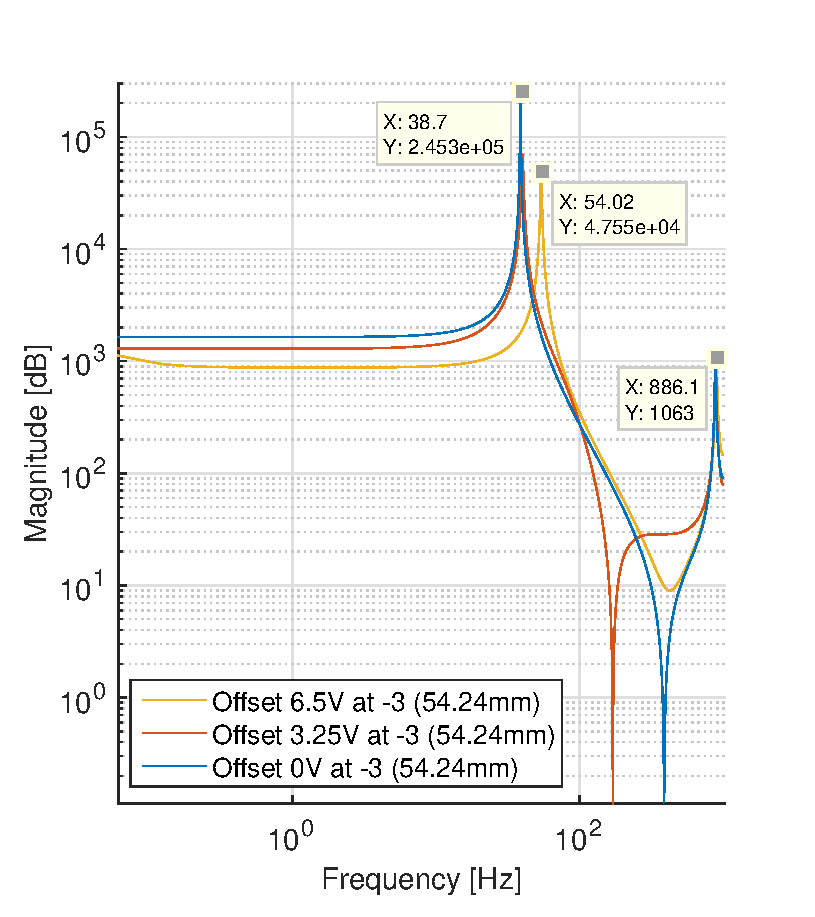
\includegraphics[width=0.46\textwidth, trim=0cm 0cm 0.8cm 0cm, clip=true]{fig/matlab/modelcomparison_diffvolt2.eps}}
  \qquad
  \subfloat[][\label{fig:different_lin_pos}Different linear axis positions]{
  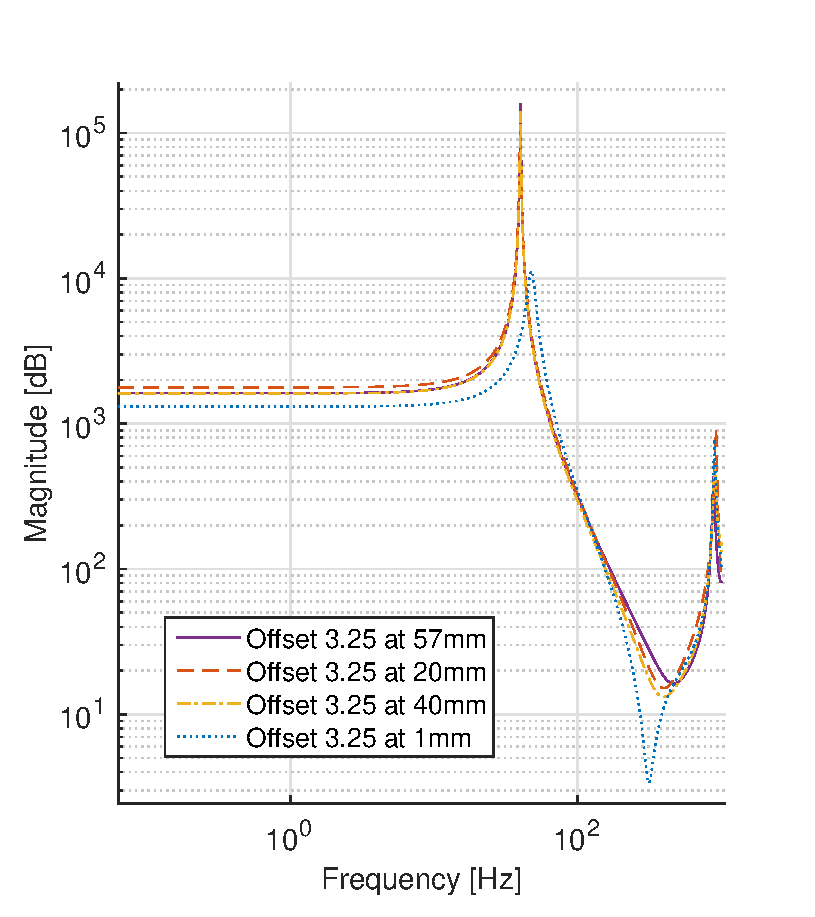
\includegraphics[width=0.46\textwidth, trim=0cm 0cm 0.8cm 0cm, clip=true]{fig/matlab/modelcomparison2.eps}}
  \caption{\label{fig:different_lin_angle} Identified models with different rotational positions (a) and linear axis positions (b).}
\end{figure}

Since the rotational stage controller needs to maintain the required tracking error even when the linear axis is moving, the disturbance during linear operation must be considered. Figure~\ref{fig:dist_diff_speed} shows the open loop response when the linear axis is moving. This figure shows how the operating speed of the stepping motor influences the spectrum of the angle with its different harmonics.

\begin{figure}[h!]
  \centering %crop: left bottom right top
  \subfloat[][\label{fig:dist_diff_speed_overview}Open loop response]{
  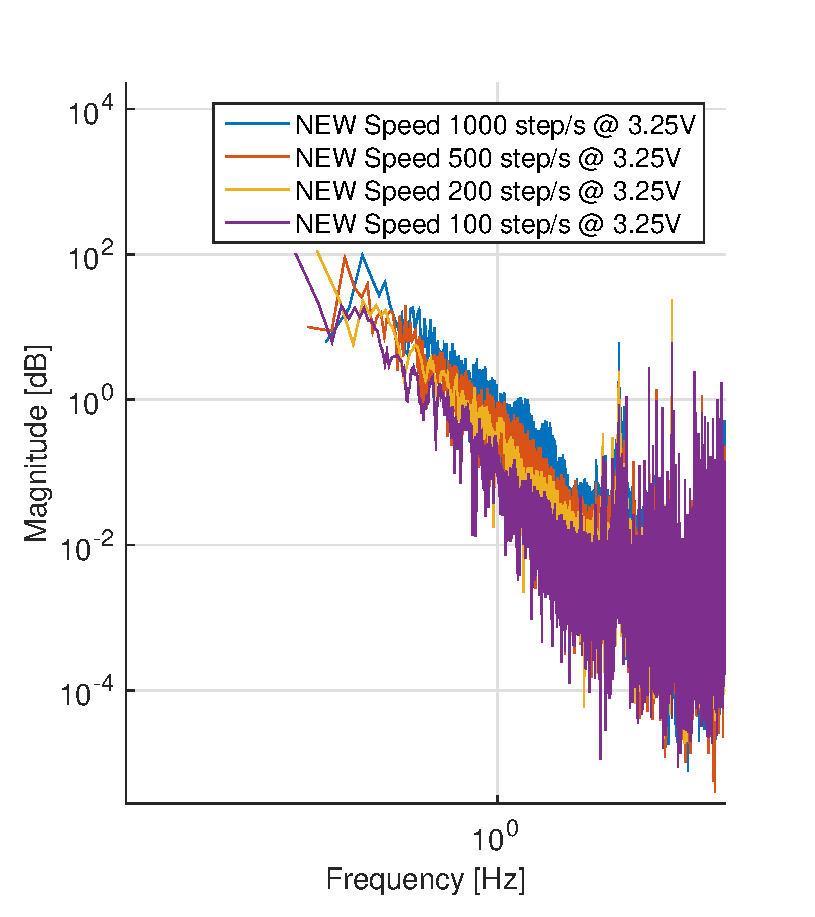
\includegraphics[width=0.46\textwidth, trim=0cm 0cm 0.8cm 0cm, clip=true]{fig/matlab/differentspeeds2.eps}}
  \qquad
  \subfloat[][\label{fig:dist_diff_speed_zoomin}Zoom in]{
  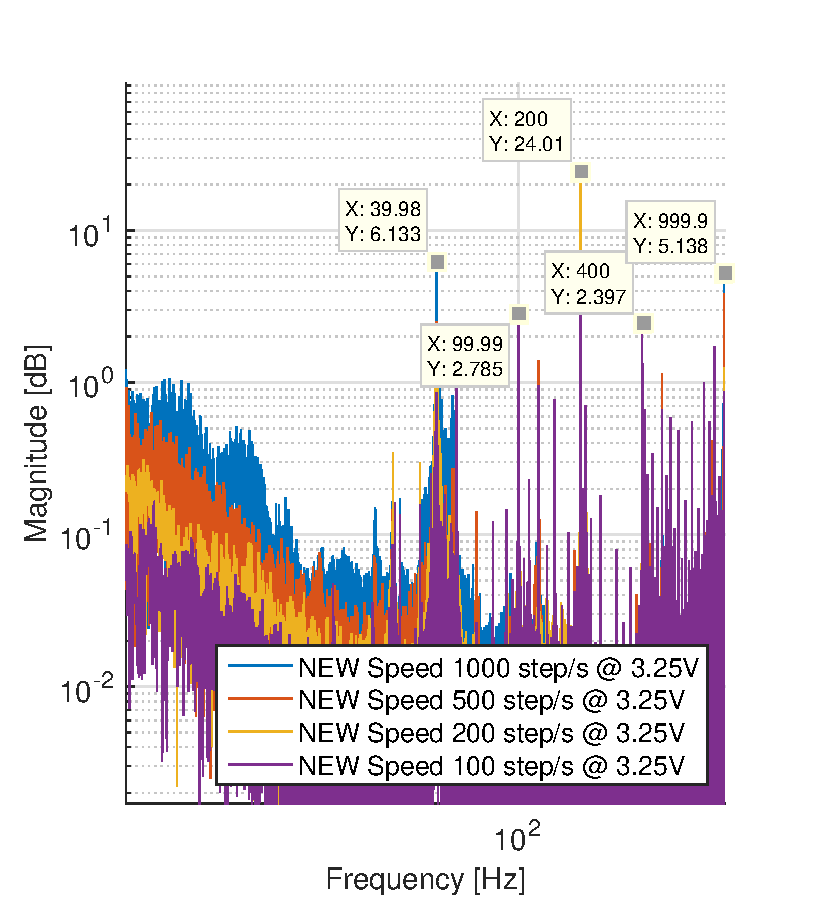
\includegraphics[width=0.46\textwidth, trim=0cm 0cm 0.8cm 0cm, clip=true]{fig/matlab/differentspeeds_Zoomin2.eps}}
  \caption{\label{fig:dist_diff_speed} The resulting responses is shown in (a) with the model change in (b).}
\end{figure}

\newpage
\FloatBarrier
\section{Model Reference Adaptive Control}
Even though the rotational stage has been modeled by \eqref{eq:tf}, a second order model approximating the higher order system was used in the adaptive control laws to keep the computational burden low. The discretized reference model can be seen in \eqref{eq:sys_gm} and all parameters and tuning variables are summarized in Table~\ref{tab:adaptive_param}. The controller is tuned to be robust to input disturbances and model changes. The set of parameter presented in Table~\ref{tab:adaptive_param} is not an optimal set but a decent set of parameters that maintains stability for step sizes below 20mrad.

\begin{equation}
  \label{eq:sys_gm}
  G_m(z) = \frac{7.9z + 6.7}{1313z^{2} - 2095z + 796.4}
\end{equation}

\begin{table}[h!]
  \centering
  \begin{tabular}{| l | l |}
    \hline
    Parameter & Value \\ \hline
    $T_s$ & $5 \times 10^{-4}$ \\
    $\alpha_0$ & $5.7 \times 10^{4}$ \\
    $\alpha_1$ & $7.2$ \\
    $\beta_0$ & $7.5 \times 10^{7}$ \\
    $a_0$ & $5.7 \times 10^{4}$ \\
    $a_1$ & $1 \times 10^{3}$ \\
    $b_0$ & $7.5 \times 10^{7}$ \\
    $\eta_0$ & $3 \times 10^{-2}$ \\
    $\eta_1$ & $1 \times 10^{-1}$ \\
    $\eta_2$ & $1 \times 10^{-10}$ \\
    $\eta_3$ & $1 \times 10^{-17}$ \\
    $\epsilon$ & $1 \times 10^{-8}$ \\
    $Q$ & $diag(1 \times 10^{10}, 1 \times 10^{-3})$\\
    \hline
  \end{tabular}
  \caption{\label{tab:adaptive_param} Parameters of the system model and the tuned adaptive controller.}
\end{table}

Figure~\ref{fig:step_adaptive} shows the step response to different step sizes. Here it is clear that the system becomes unstable if the step size $\geq$ \unit{26}{\milli\radian}. The controller has been tuned to handle the maximum step size, i.e the rotational range of \unit{20}{\milli\radian}, which results in a longer rise time for the smaller step sizes. The simulation was performed without any saturation on the input signal, indicating that amplitude dependent behavior might be due to numerical errors. Note that the responses are produced with initial values $k_i = 0$, if the initial values would be set to the values that $k_i$ settles to, a faster step response could be expected. This can be seen in Figure~\ref{fig:periodic_resp} where the controller performs better for the second period.

\begin{figure}[h!]
  \centering
  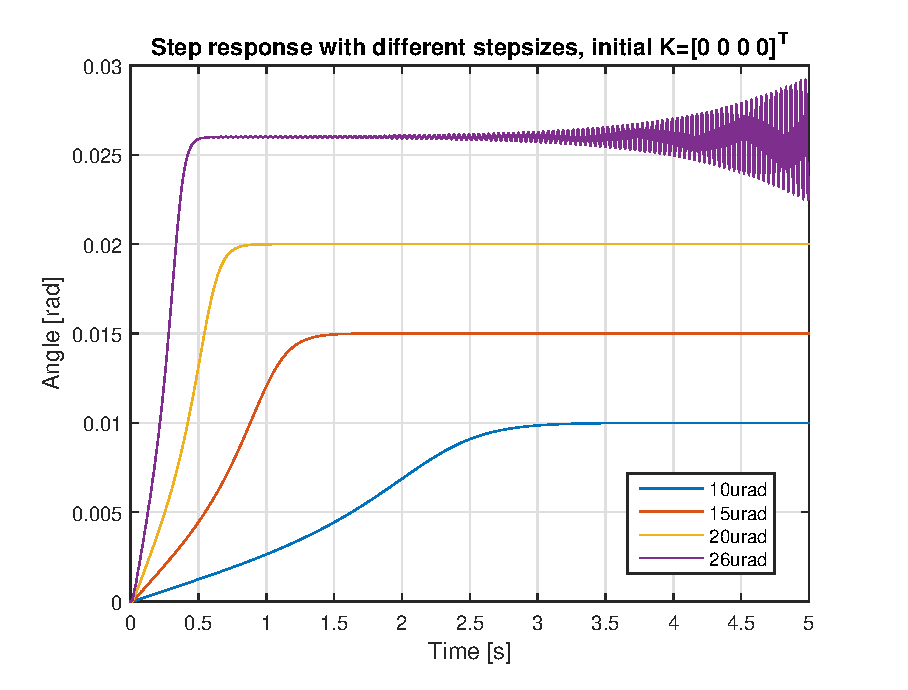
\includegraphics[width=0.7\textwidth]{fig/matlab/stepresponse.eps}
  \caption{\label{fig:step_adaptive} Step responses to step sizes of 10, 15, 20 and 26 mrad.}
\end{figure}

The adaptation process of the control parameters $k_i$, for a step response resulting from a 20mrad step, can be seen in Figure~\ref{fig:adapt_process}. All of the coefficients have converged within 1 second.

\begin{figure}[h!]
  \centering
  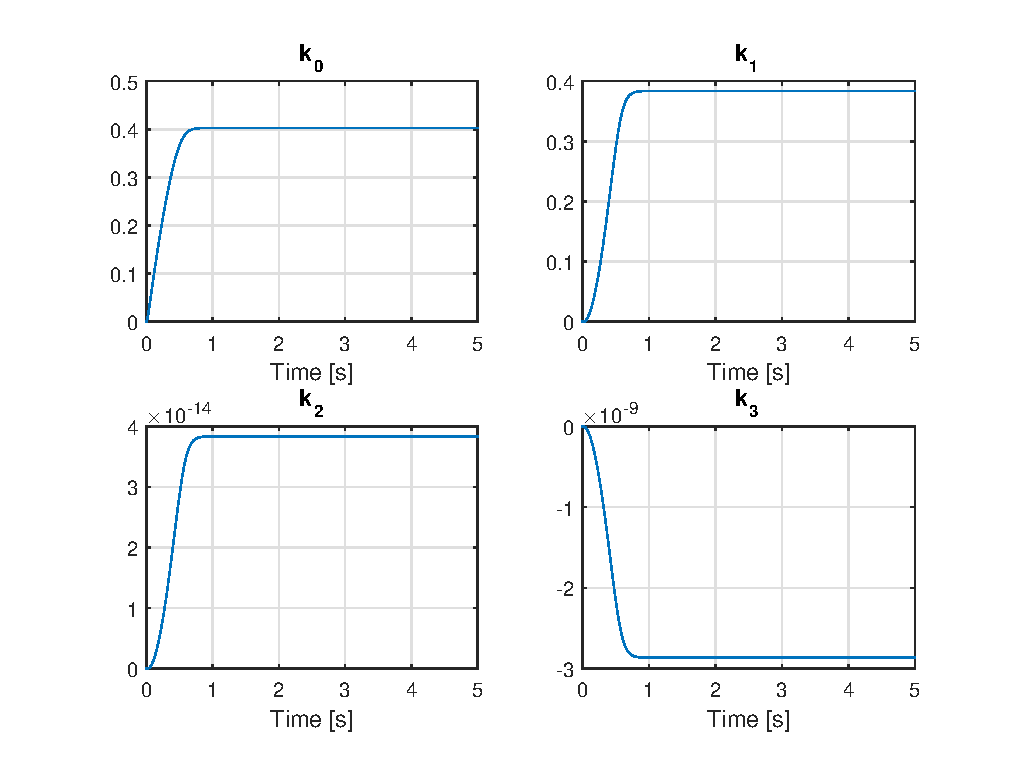
\includegraphics[width=1\textwidth]{fig/matlab/k.eps}
  \caption{\label{fig:adapt_process} Adaptation process of control parameters $k_i$ with a 20 mrad step.}
\end{figure}

\FloatBarrier
To illustrate the adaptation process better, a periodic response is depicted in Figure~\ref{fig:periodic_resp} where it is clear that after the adaptation process is finished the controller performs better for the second and third period. One can see that the adaptation process is slower for the periodic response corresponding to the amplitude of \unit{10}{\milli\radian}, hence the lower the step, the longer the adaptation time. The present controller performs well for all amplitudes.

\begin{figure}[h!]
  \centering
  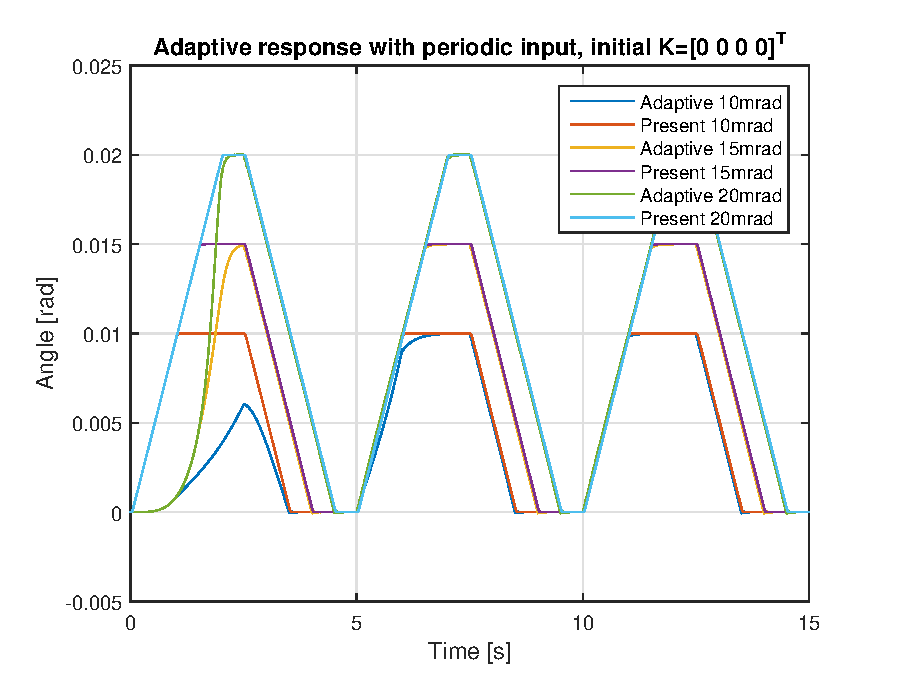
\includegraphics[width=0.7\textwidth]{fig/matlab/periodicresponse.eps}
  \caption{\label{fig:periodic_resp} Periodic responses for the adaptive and present controller with amplitudes of 10, 15, 20 mrad.}
\end{figure}

\begin{figure}[h!]
  \centering
  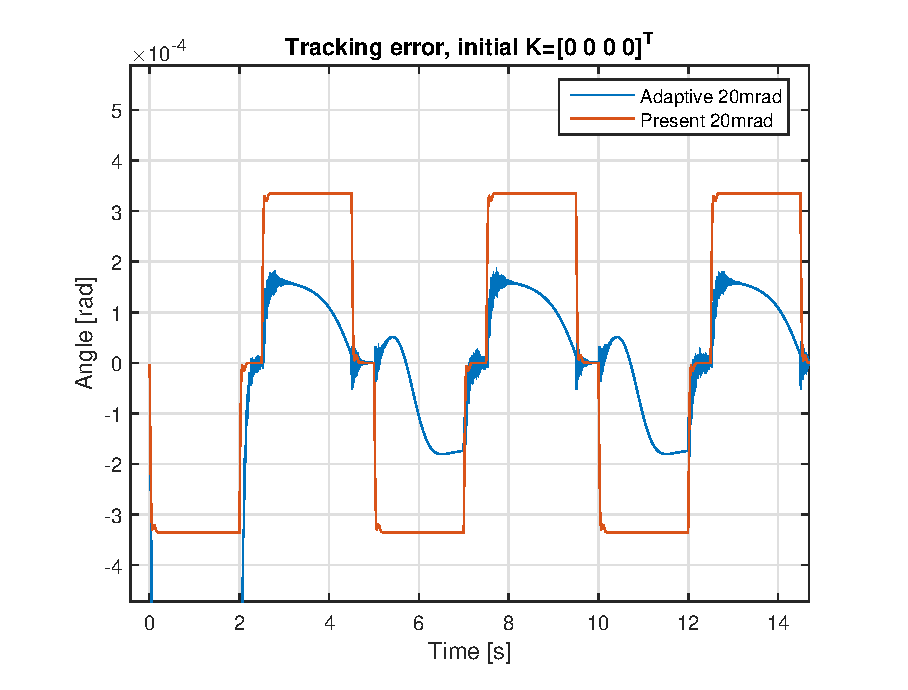
\includegraphics[width=0.7\textwidth]{fig/matlab/trackingerror.eps}
  \caption{\label{fig:adapt_trackingerror} Tracking error (difference between reference and output) for the periodic response from an input signal with an amplitude of 20 mrad.}
\end{figure}

The tracking error corresponding to the \emph{Adaptive 20mrad} and \emph{Present 20mrad} in Figure~\ref{fig:periodic_resp} can be seen in Figure~\ref{fig:adapt_trackingerror}. The adaptive controller performs better than the present controller after the adaptation process has finished.

A periodic response with model parameter drift is presented in Figure~\ref{fig:modeldrift}. It shows how the adaptive controller manages to adapt to the change in the system dynamics, while the present controller fails to do so, resulting in an unstable system. The change of the model was performed over 2 seconds, resulting in a movement of the first resonance peak, from 38 Hz to 66 Hz in frequency and from 30.1 dB to 23.5 dB in magnitude. Note that the change of the model is relatively big and for a smaller movement of the resonance peak, the present controller could still be sufficient as illustrated in Figure~\ref{fig:modelerror}.
\begin{figure}[h!]
  \centering %crop: left bottom right top
  \subfloat[][\label{fig:modeldriftresponse}Periodic response with model parameter drift.]{
  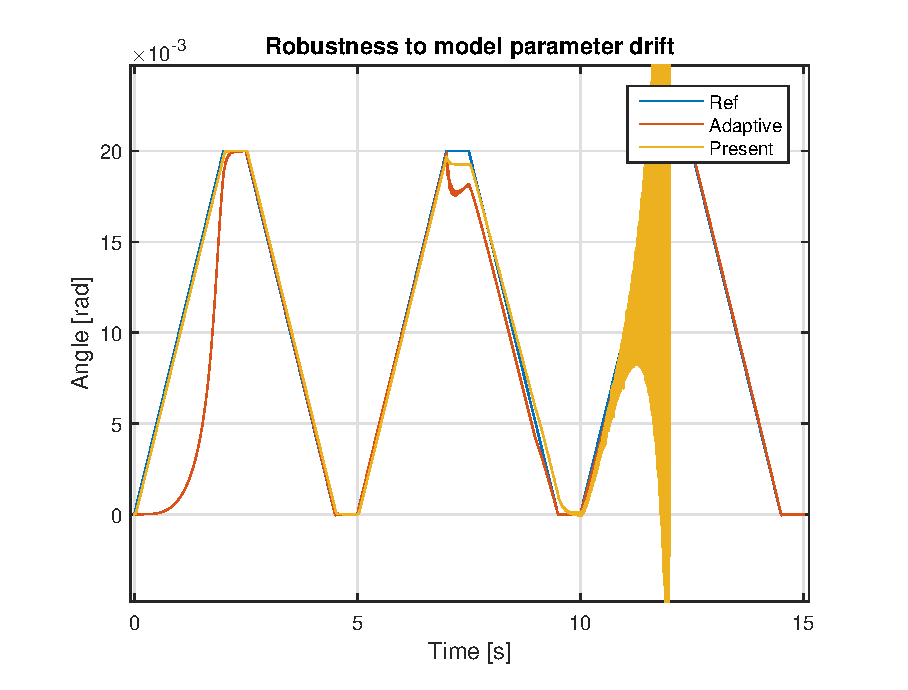
\includegraphics[width=0.46\textwidth, trim=0cm 0cm 1cm 0cm, clip=true]{fig/matlab/driftofmodelparameterover2s.eps}}
  \qquad
  \subfloat[][\label{fig:modeldriftbode}Original model (G) and the resulting model after drift ($G_{mod}$).]{
  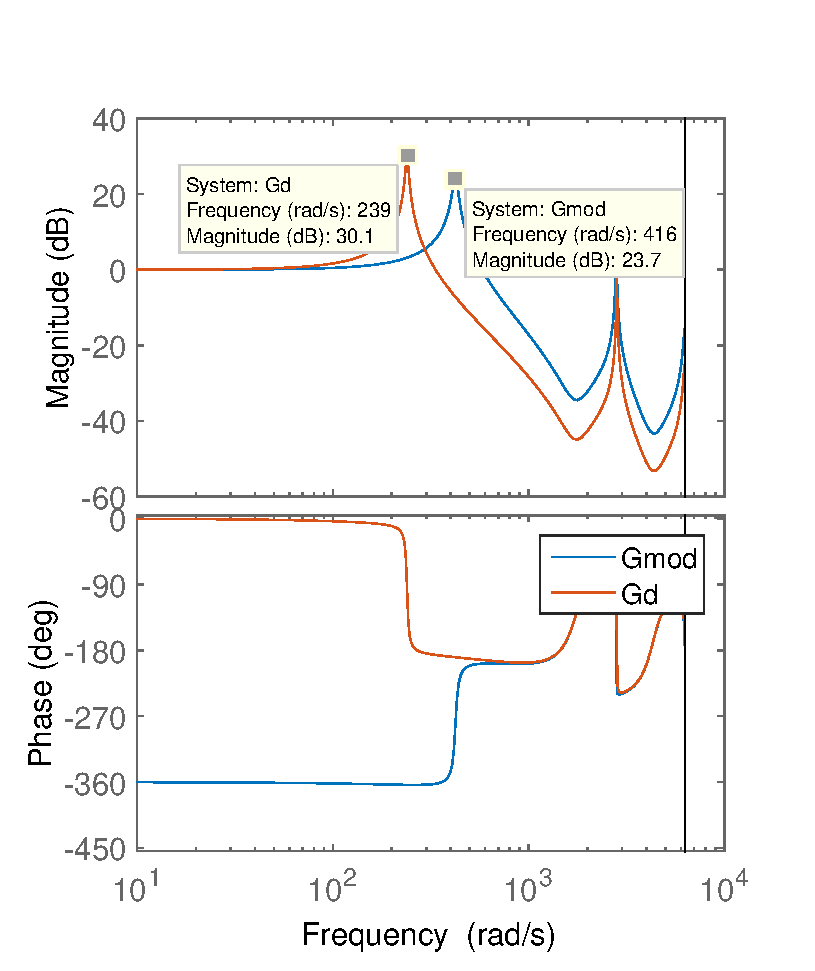
\includegraphics[width=0.46\textwidth, trim=0cm 0cm 0.7cm 0cm, clip=true]{fig/matlab/bode_drift_pole.eps}}
  \caption{\label{fig:modeldrift} Shows the robustness to model changes over time. The model error is increased linearly from $t=7s$ to $t=9s$. The resulting responses are shown in (a) with the model change in (b).}
\end{figure}

\begin{figure}[h!]
  \centering %crop: left bottom right top
  \subfloat[][\label{fig:modelerrorresponse}Periodic response with model parameter drift.]{
  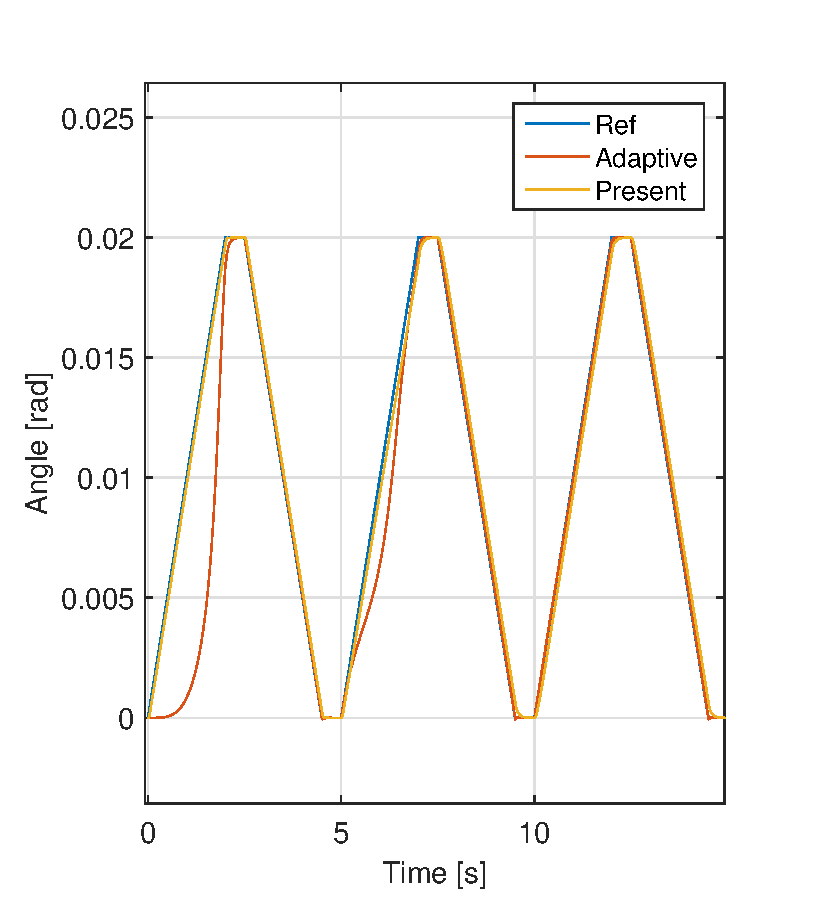
\includegraphics[width=0.46\textwidth, trim=0cm 0cm 1cm 0cm, clip=true]{fig/matlab/modelerrorperiodic.eps}}
  \qquad
  \subfloat[][\label{fig:modelerrorbode}Original model (G) and the resulting model after drift ($G_{mod}$).]{
  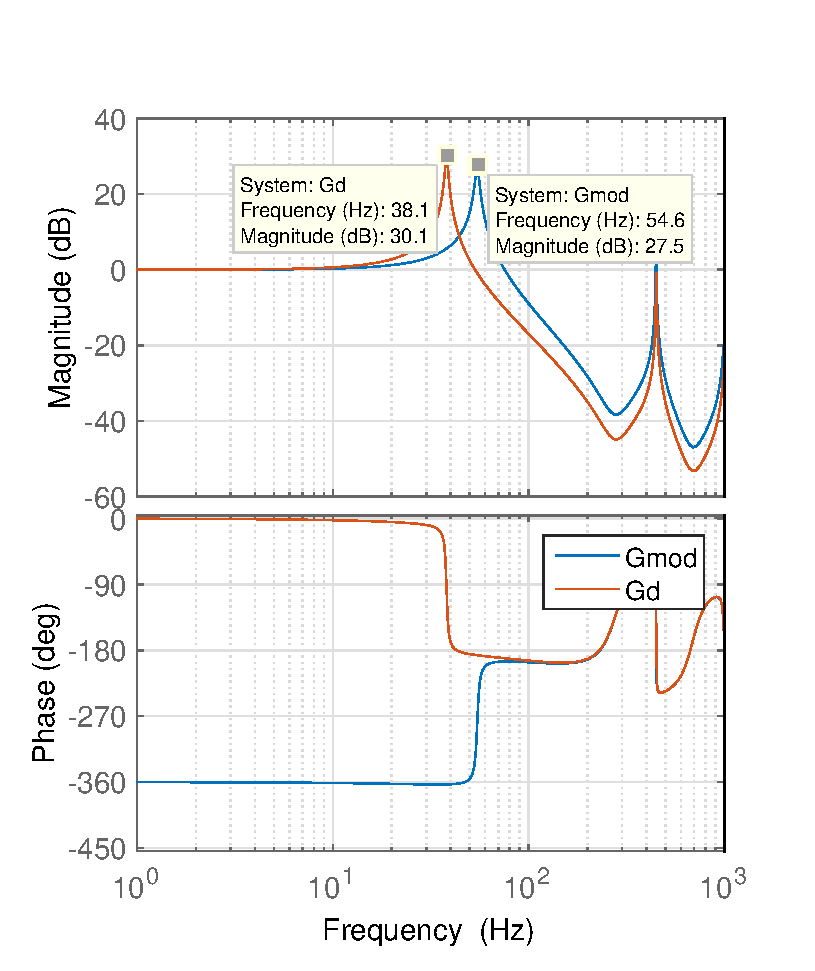
\includegraphics[width=0.46\textwidth, trim=0cm 0cm 0.7cm 0cm, clip=true]{fig/matlab/bode_modelerror_pole.eps}}
  \caption{\label{fig:modelerror}Robustness to model changes over time. The model error is increased linearly from $t=5s$ to $t=7s$. The resulting responses are shown in (a) with the model change in (b).}
\end{figure}

In the case in Figure~\ref{fig:modelerror} the resonance peak is only moved 6.5 Hz and the present controller is sufficient to suppresses the disturbance. It even does it more efficiently than the adaptive controller. Even though the adaptive is slower than the present controller it still produces a smaller tracking error after the adaption process is over, see Figure~\ref{fig:modelerror_trackingerror}. Note that the change in the model is equivalent to the change between 0V and 6.5V presented in Figure~\ref{fig:different_angles}.

\begin{figure}[h!]
  \centering
  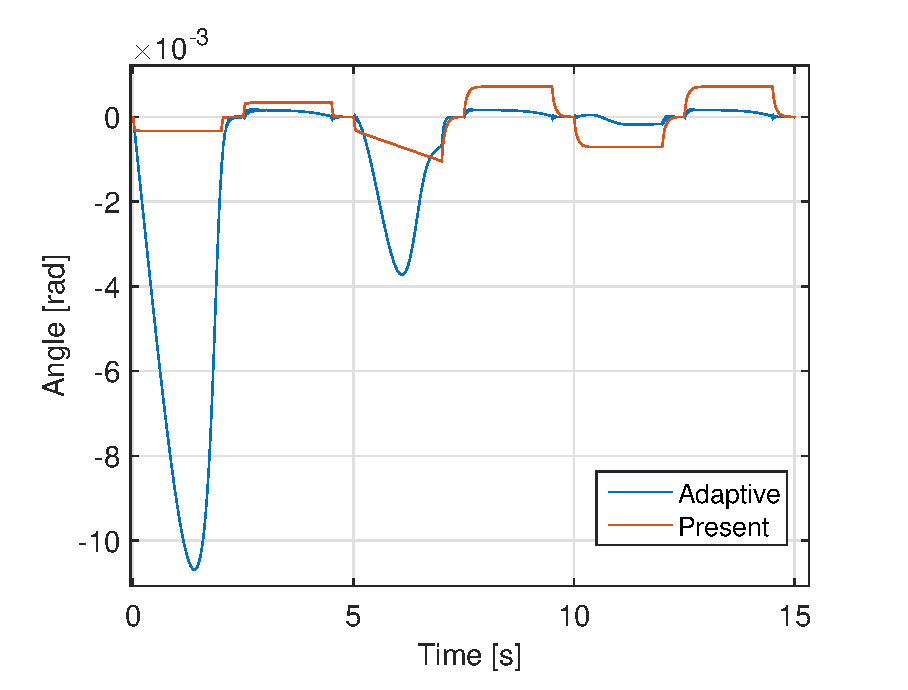
\includegraphics[width=0.7\textwidth]{fig/matlab/modelerrorperiodic_trackingerror.eps}
  \caption{\label{fig:modelerror_trackingerror} Tracking error for the periodic response with a model error drift from $t=5s$ to $t=7s$.}
\end{figure}

\FloatBarrier
Figure~\ref{fig:distrejection} and \ref{fig:distmeasrejection} shows the disturbance rejection capability to a disturbance on the input and output, respectively. In Figure~\ref{fig:distrejection} a small impulse was added to the input to see if the controllers would attenuate it sufficiently. The adaptive controller performed worse than the present controller both with and without prefilter. The present controller managed to attenuate the highest peak of the impulse by 1.5 times more than the adaptive. The settling time was also approximately 3 times worse for the adaptive controllers. In Figure~\ref{fig:distmeasrejection} the impulse was instead added to the measured signal. Even in this case the present controller was superior, attenuating the highest peak of the impulse by 3 times more than the adaptive controller.

\begin{figure}[h!]
  \centering %crop: left bottom right top
  \subfloat[][\label{fig:dist}Step response]{
  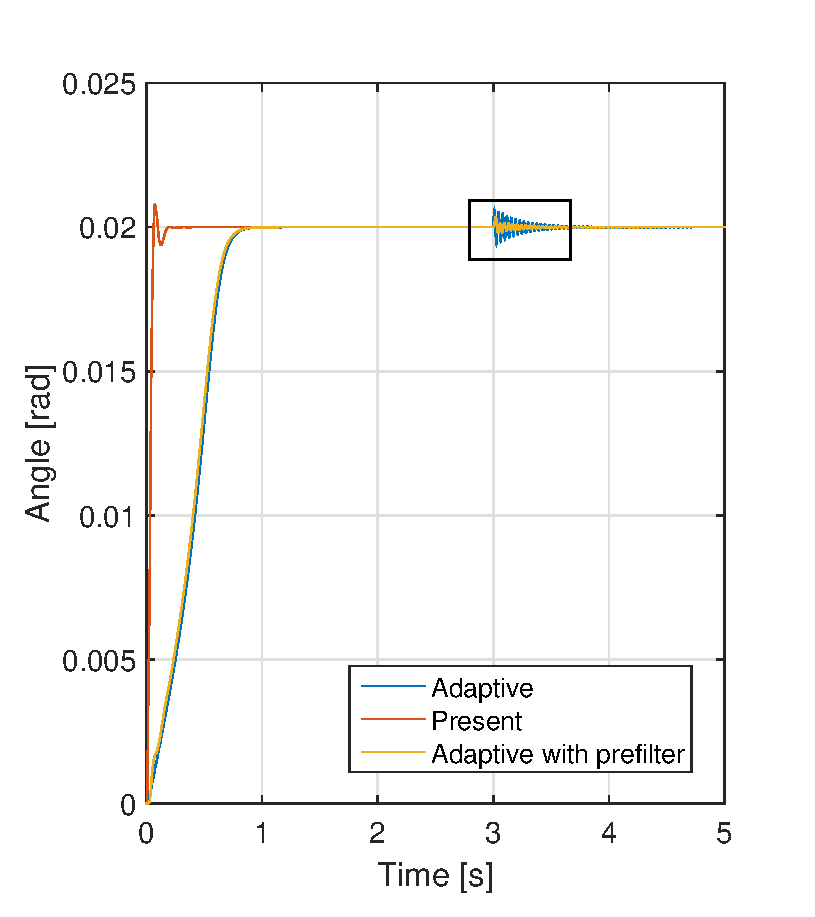
\includegraphics[width=0.46\textwidth, trim=0cm 0cm 1cm 0.8cm, clip=true]{fig/matlab/distrejection.eps}}
  \qquad
  \subfloat[][\label{fig:distzoom}Zoom in on disturbance]{
  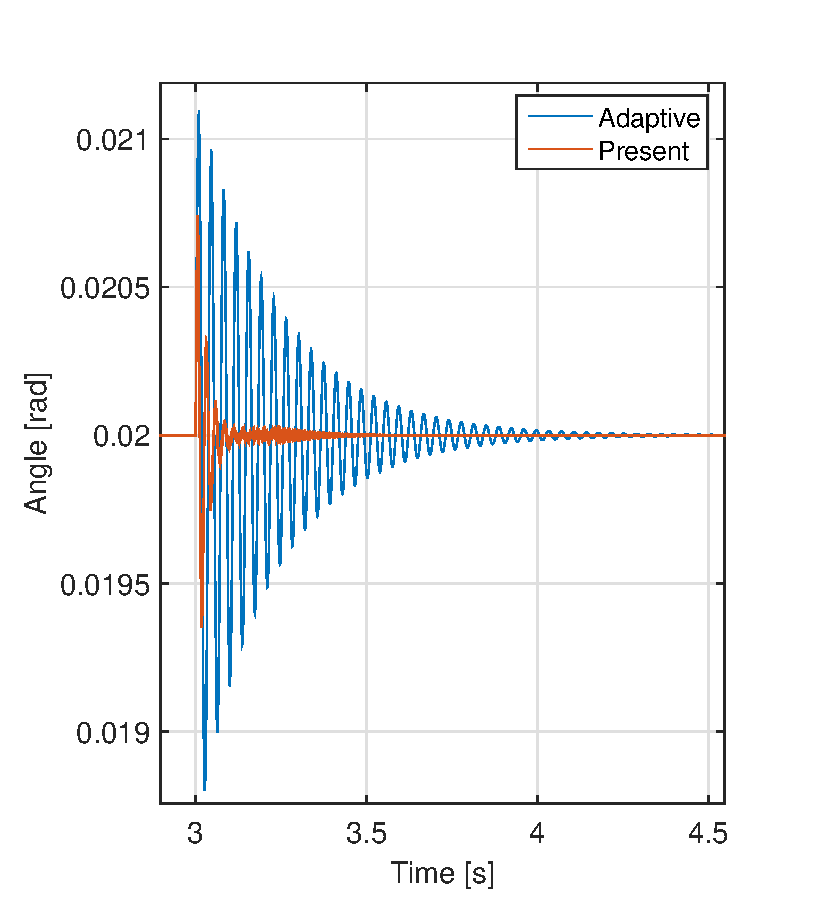
\includegraphics[width=0.46\textwidth, trim=0cm 0cm 1cm 0.8cm, clip=true]{fig/matlab/distrejection_zoom.eps}}
  \caption{\label{fig:distrejection} Controller attenuation of a disturbance impulse (amplitude of $5.1 \times 10^{-3}$) added to the input signal at $t=3s$. The whole step response is shown in (a) with a zoom in on the disturbance in (b).}
\end{figure}
\begin{figure}[h!]
  \centering %crop: left bottom right top
  \subfloat[][\label{fig:distmeas}Step response]{
  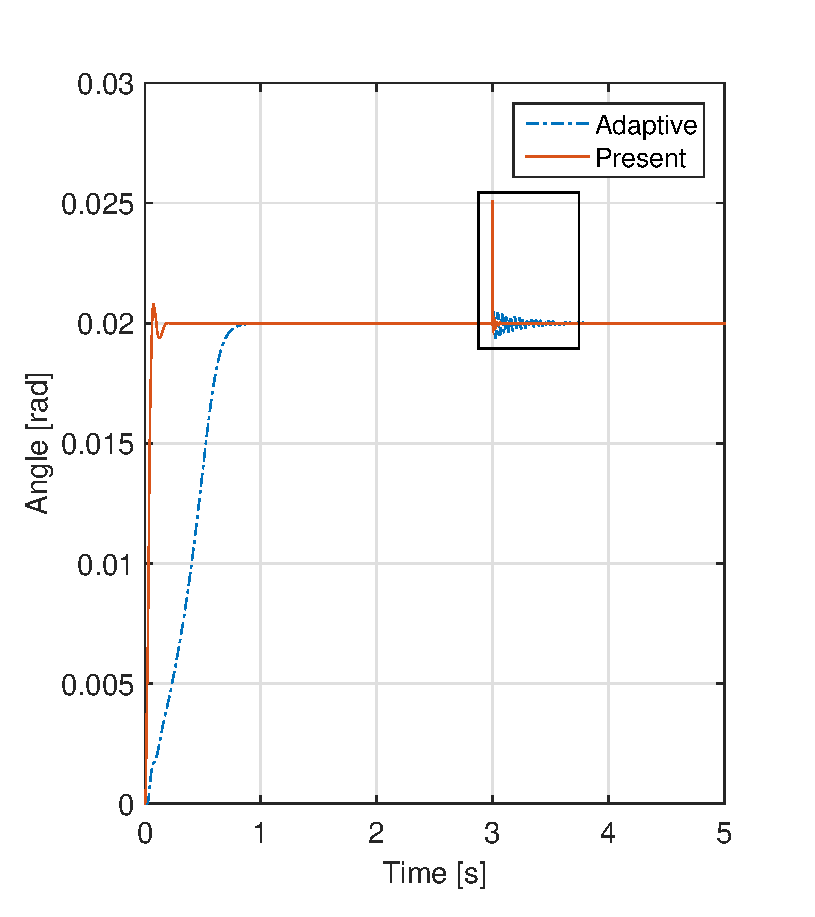
\includegraphics[width=0.46\textwidth, trim=0cm 0cm 1cm 0.8cm, clip=true]{fig/matlab/distrejection_meas.eps}}
  \qquad
  \subfloat[][\label{fig:distmeaszoom}Zoom in on disturbance]{
  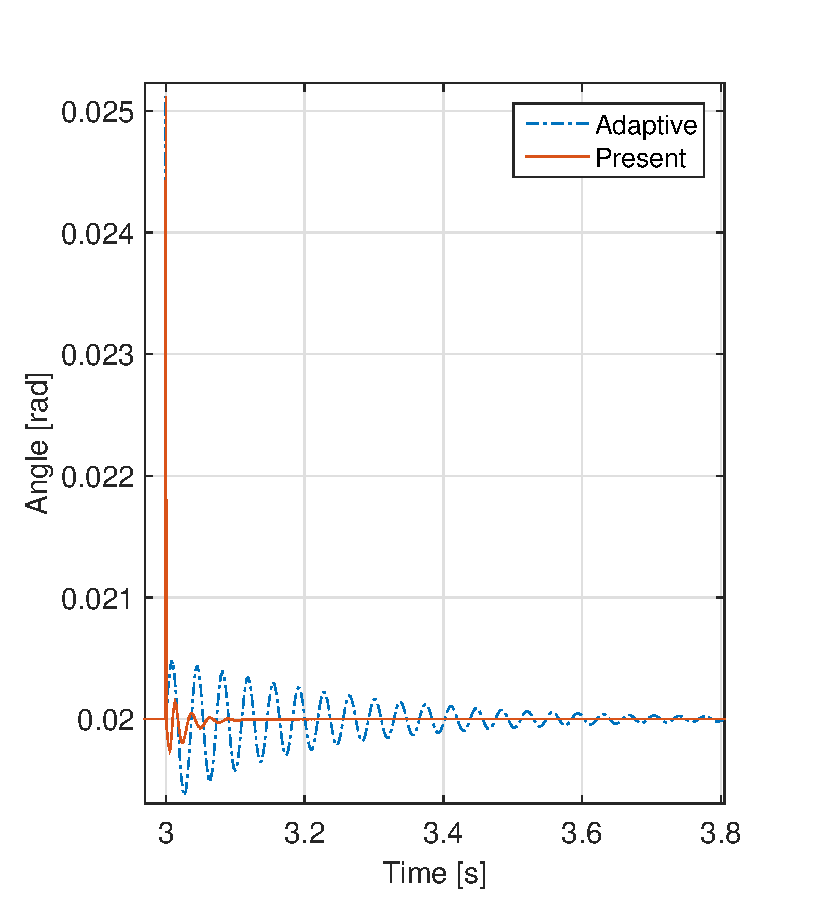
\includegraphics[width=0.46\textwidth, trim=0cm 0cm 1cm 0.8cm, clip=true]{fig/matlab/distrejection_meas_zoom.eps}}
  \caption{\label{fig:distmeasrejection} Disturbance rejection to impulses (amplitude of $5.1 \times 10^{-3}$) added to the measured signal at $t=3s$. The step response is shown in (a)  with a zoom in on the disturbance in (b).}
\end{figure}

\newpage~\newpage~
\FloatBarrier
\section{Integral Resonance Control}
The \abbrIRC design procedure presented in \ref{sec:irc} was carried out in continuous time, but each block in the scheme was individually discretized for the sake of comparison with the present controller. The continuous time representation of the system in \eqref{eq:tf} contains 7 poles and 6 zeros i.e. a relative degree of 1. A negative feedforward would therefore introduce another zero that can be placed in a desired position by adjusting the gain $D_f$. As seen in the pole-zero plot comparison in Figure~\ref{fig:negfeedpzmap}, a feedforward of $D_f=-1.2$ was sufficient to introduce one zero and place it and its complex conjugate below the first resonance frequency. This and the zero-pole interlacing for the higher order modes can be seen in Figure~\ref{fig:pzafter}, where the zoom-in shows the complex conjugate zeros below the first resonance mode.

\begin{figure}[h!]
  \centering %crop: left bottom right top
  \subfloat[][\label{fig:pzbefore}Origianl system]{
  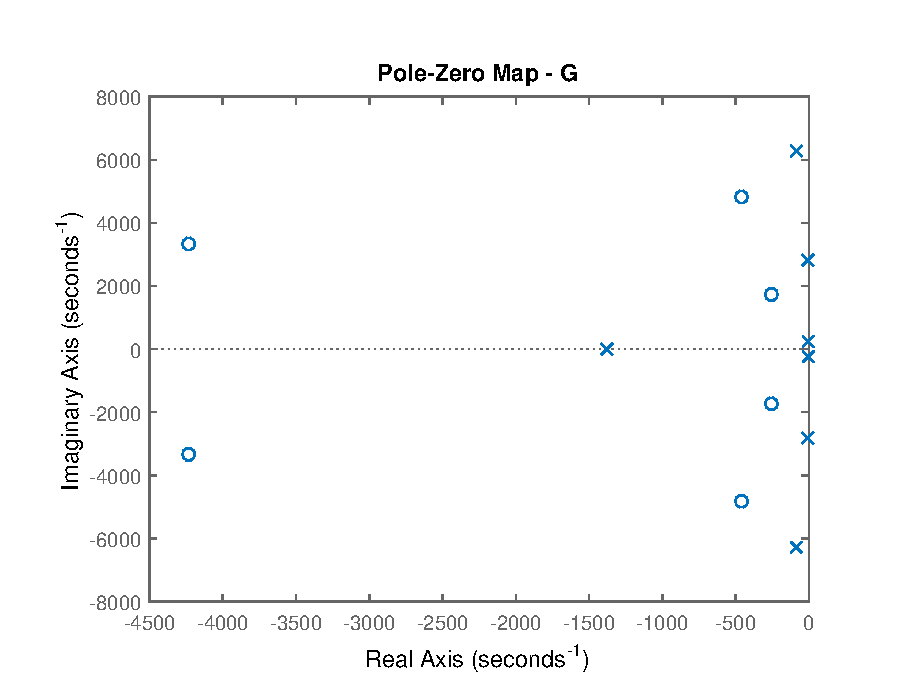
\includegraphics[width=0.46\textwidth, trim=0cm 0cm 1cm 0cm, clip=true]{fig/matlab/pzbefore.eps}}
  \qquad
  \subfloat[][\label{fig:pzafter}After feedforward]{
  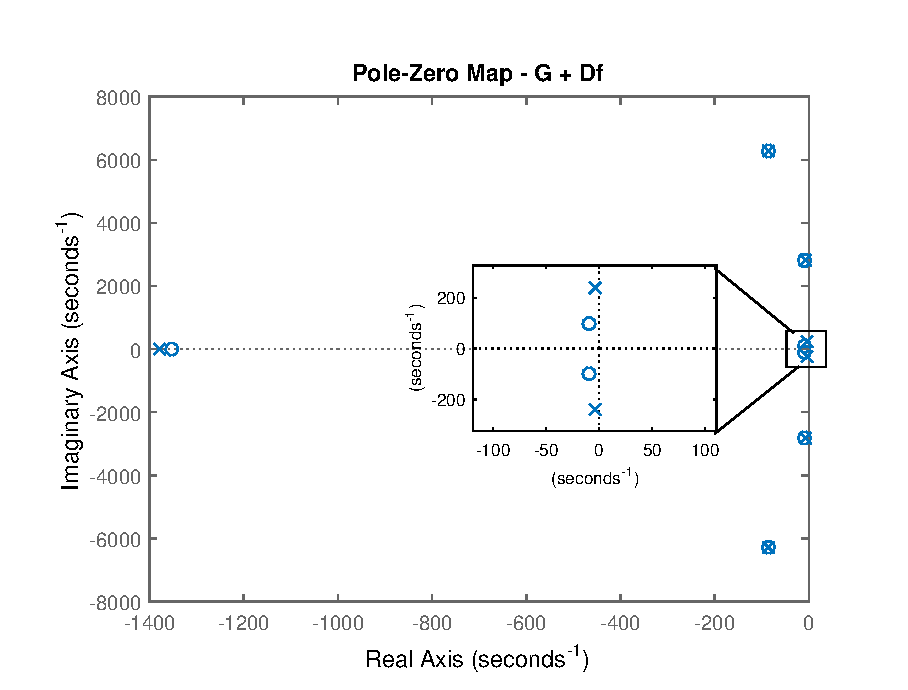
\includegraphics[width=0.46\textwidth, trim=0cm 0cm 1cm 0cm, clip=true]{fig/matlab/pzafter.eps}}
  \caption{\label{fig:negfeedpzmap} Comparison of pole-zero plot before and after adding the negative feedforward. After adding the feedforward to the system which poles and zeros are shown in (a) , the zeros and poles are interlacing as seen in (b).}
\end{figure}
\FloatBarrier
The corresponding Bode plot can be seen in Figure~\ref{fig:bodeafterfeedf}, showing the complex conjugate pair of zeros as a dip before the first resonance peak.

\begin{figure}[h!]
  \centering
  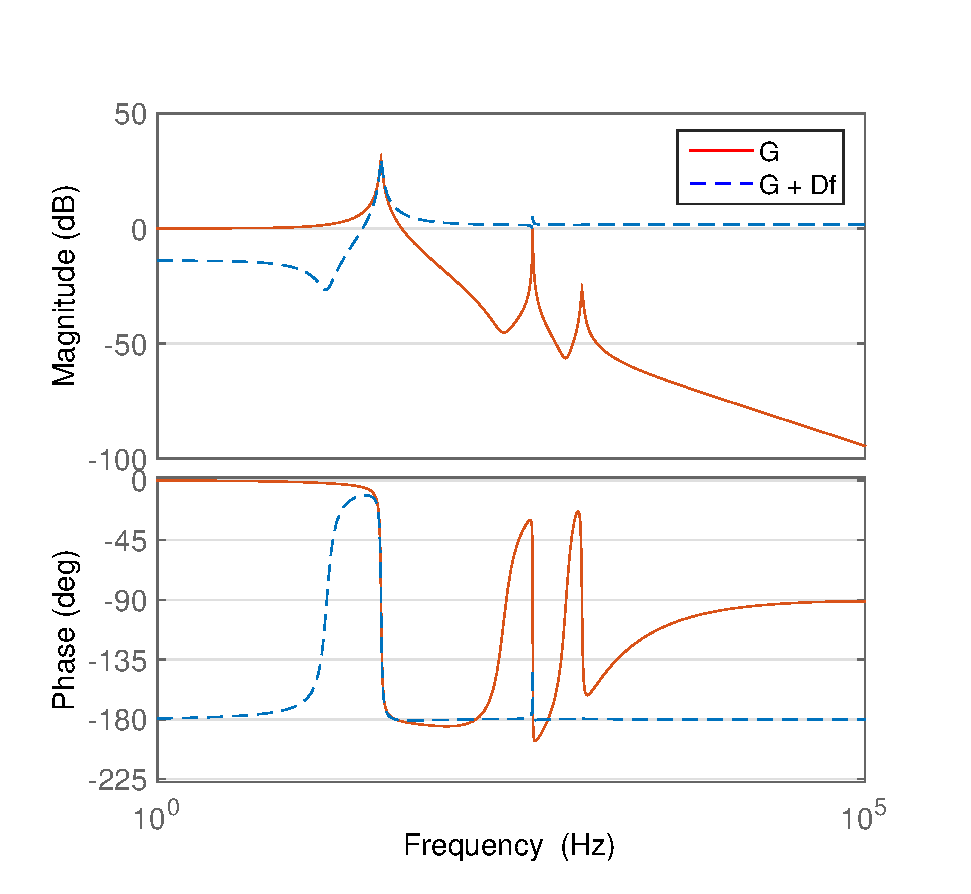
\includegraphics[width=0.7\textwidth]{fig/matlab/bodeafterfeedf.eps}
  \caption{\label{fig:bodeafterfeedf} Bode plot of the system before and after the addition of the negative feedforward.}
\end{figure}

\FloatBarrier
The integral controller $C=\frac{-k}{s}$ was added according to Section~\ref{sec:irc} and a gain of $k=314$ was found to maximize the damping, by using the root locus technique.
The open and closed loop system of the \abbrIRC damping loop depicted in Figure~\ref{fig:irc} is shown in Figure~\ref{fig:bodedamped}. It is clear that the integral controller damps out the first resonance peak efficiently in closed loop.

\begin{figure}[h!]
  \centering
  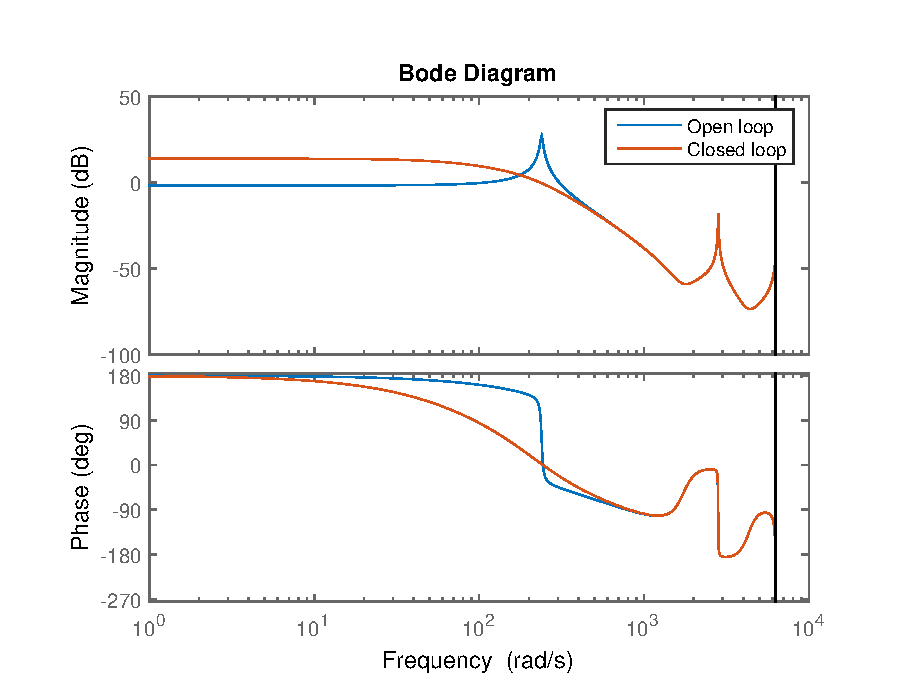
\includegraphics[width=0.7\textwidth]{fig/matlab/bodedamped.eps}
  \caption{\label{fig:bodedamped} Open and closed loop of the IRC damping loop.}
\end{figure}

Finally, the damped system was enclosed in an outer loop with a second controller $C_1$ for reference tracking capability. $C_1$ was designed to be robust to model errors i.e. keep the sensitivity function $G_{dy}$, stated in \eqref{eq:Gyd}, low for the frequencies that the model changes with, (d and y in $G_{dy}$ can be found in the block scheme in Figure~\ref{fig:irc_int}). It was also designed to attenuate higher order resonances using an inclusion of a notch filter.  $C_1$ was designed in Matlab's SISO-Tool and is presented in \eqref{eq:C_1}.

\begin{equation}
  \label{eq:Gyd}
  G_{yd} = \frac{1}{1 + C_2G(1 + C_1)}
\end{equation}

\begin{equation}
  \label{eq:C_1}
  C_1 = \frac{-13.54 z^5 + 40.92 z^4 - 57.47 z^3 + 55.89 z^2 - 35.87 z + 10.05}{z^5 - 1.65 z^4 + 0.80 z^3 - 0.16 z^2 + 0.014 z - 0.00042}
\end{equation}

The resulting closed loop system and the sensitivity function is shown in Figure~\ref{fig:irc_totalclosed} and \ref{fig:sensitivity_irc}, respectively. The plots show that the use of the \abbrIRC has increased the closed loop bandwidth from 11 Hz to 73 Hz, corresponding to an increase of 6.5 times the present closed loop bandwidth.

\begin{figure}[h!]
  \centering
  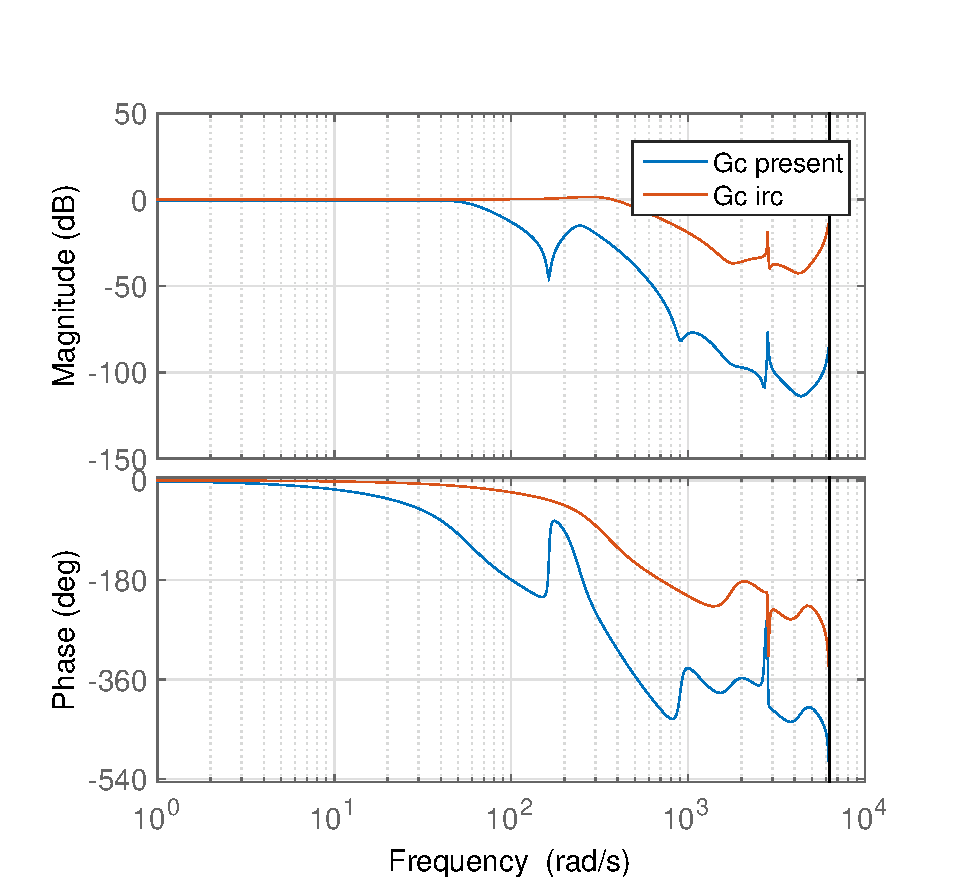
\includegraphics[width=0.7\textwidth]{fig/matlab/totalclosedloop.eps}
  \caption{\label{fig:irc_totalclosed} Closed loop system of the \abbrIRC and the present approach}
\end{figure}

The \abbrIRC sensitivity function also shows that the \abbrIRC scheme attenuates model disturbances better in the low frequency range and in the region within 24-64 Hz.

\begin{figure}[h!]
  \centering
  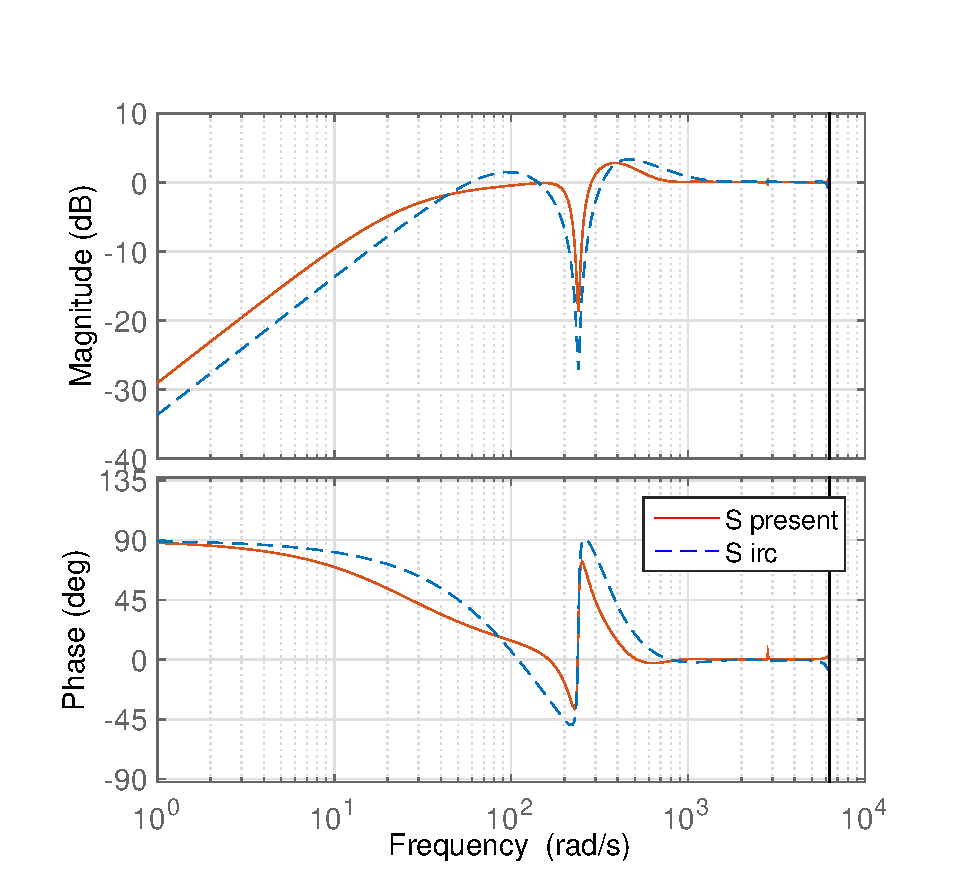
\includegraphics[width=0.7\textwidth]{fig/matlab/sensitivity_irc.eps}
  \caption{\label{fig:sensitivity_irc}Sensitivity function ($G_{dy}$) of the \abbrIRC and the present approach}
\end{figure}

\FloatBarrier
The \abbrIRC tracking performance is shown in Figure~\ref{fig:irc_tracking}. One can conclude that neither the present nor the \abbrIRC eliminate the constant ramp tracking error. However the \abbrIRC performs better due to its high bandwidth, see Figure~\ref{fig:irc_periodic} for the response and the tracking error in Figure~\ref{fig:irc_tracking}.

\begin{figure}[h!]
  \centering %crop: left bottom right top
  \subfloat[][\label{fig:irc_periodic}Periodic Response]{
  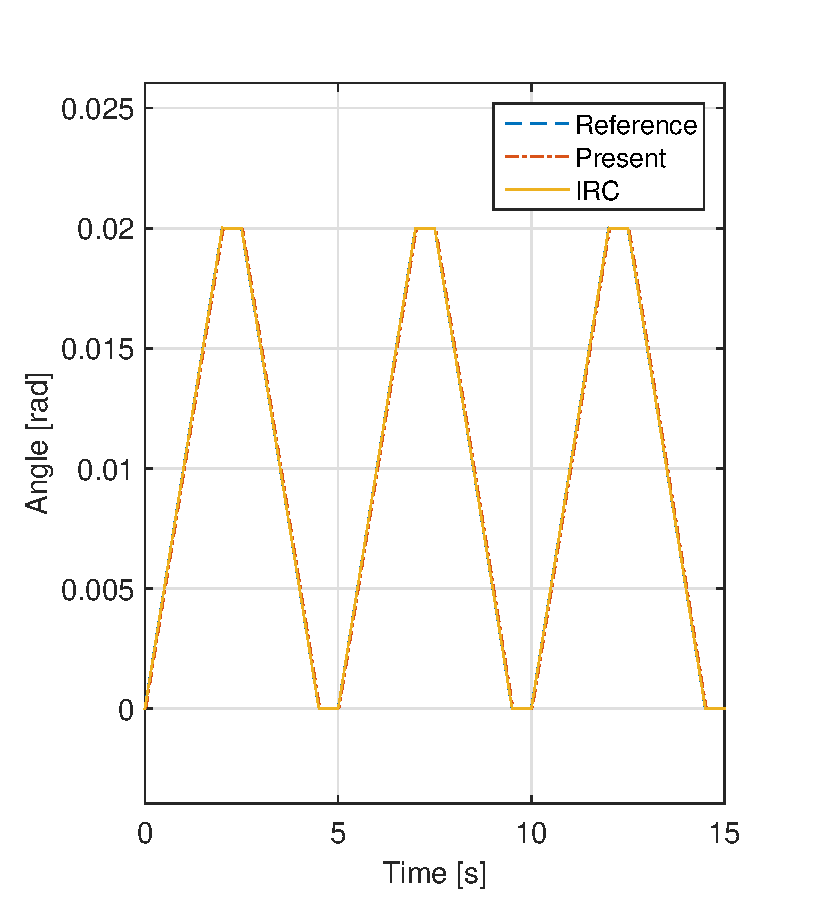
\includegraphics[width=0.46\textwidth, trim=0cm 0cm 1cm 0cm, clip=true]{fig/matlab/irc_periodic.eps}}
  \qquad
  \subfloat[][\label{fig:irc_tracking_error}Tracking error]{
  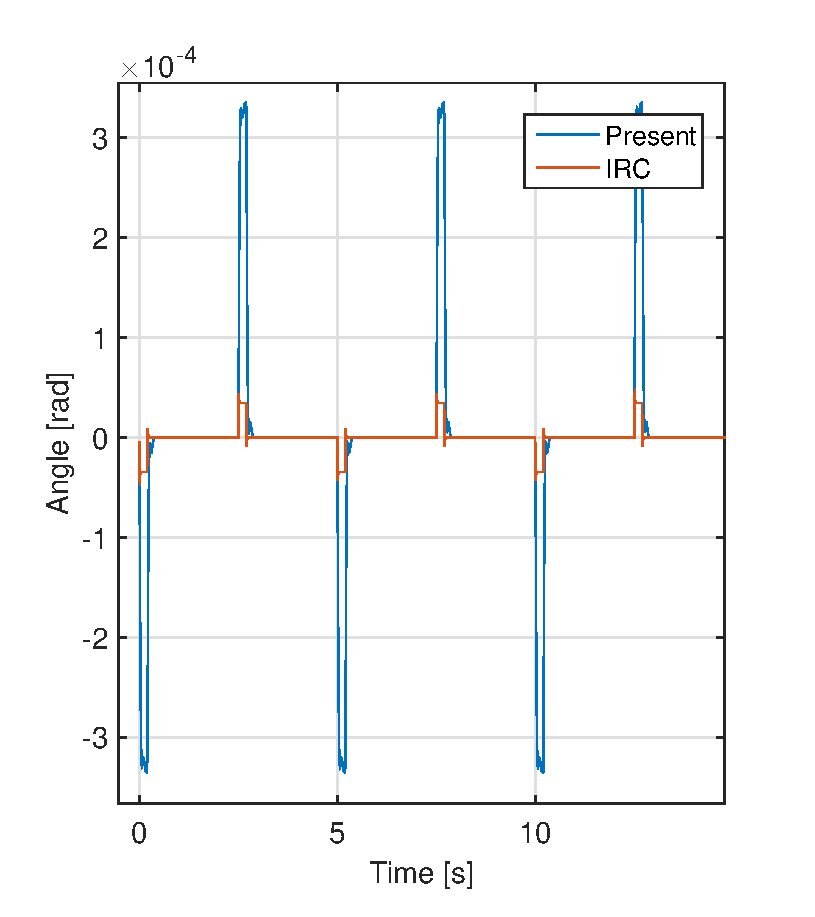
\includegraphics[width=0.46\textwidth, trim=0cm 0cm 1cm 0cm, clip=true]{fig/matlab/irctrackingerror.eps}}
  \caption{\label{fig:irc_tracking} A zoom on one period of the periodic response is shown in (a) while a the tracking error over three periods are shown in (b).}
\end{figure}

The robustness test performed for the adaptive controller was done for the \abbrIRC controller accordingly. Figure~\ref{fig:irc_dist_model} shows the periodic response and its tracking error when the model is changed linearly according to Figure~\ref{fig:modelerrorbode}. The \abbrIRC handles the model drift better than the present controller.

\begin{figure}[h!]
  \centering %crop: left bottom right top
  \subfloat[][\label{fig:irc_dist_model}Periodic response]{
  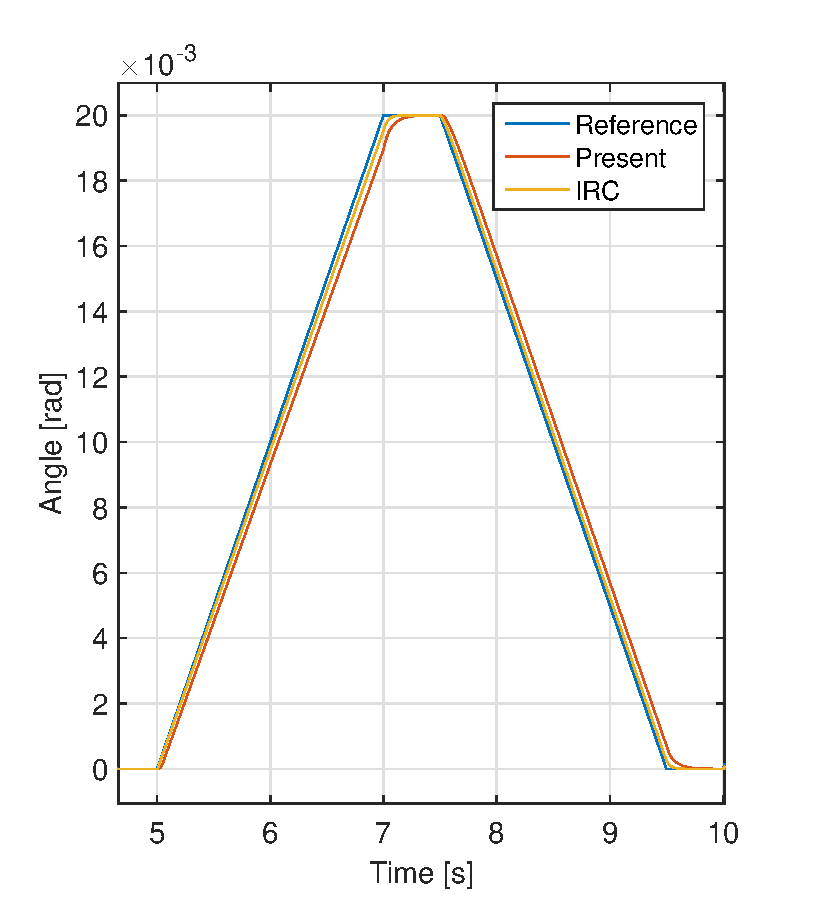
\includegraphics[width=0.46\textwidth, trim=0cm 0cm 1cm 0cm, clip=true]{fig/matlab/irc_periodic_drift.eps}}
  \qquad
  \subfloat[][\label{fig:irc_dist_model_drift}Periodic response with model parameter drift.]{
  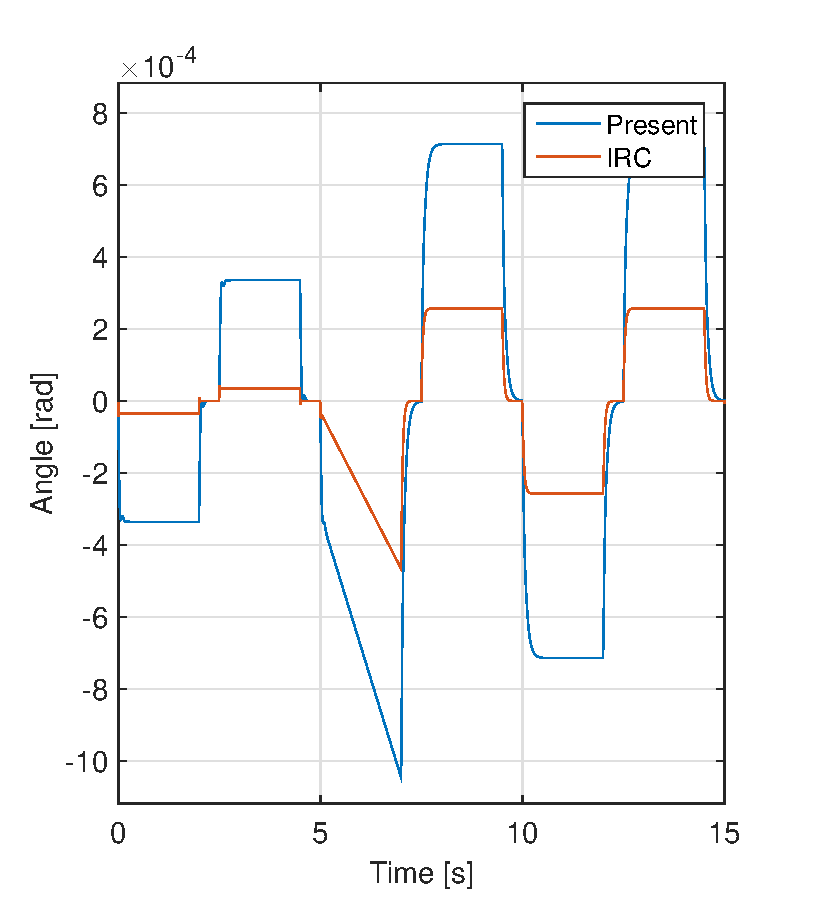
\includegraphics[width=0.46\textwidth, trim=0cm 0cm 1cm 0cm, clip=true]{fig/matlab/irc_periodic_trackingerror.eps}}
  \caption{\label{fig:irc_dist} Shows the robustness to model changes over time. The model error is increased linearly from $t=5s$ to $t=7s$.  A zoom in on one period is shown in (a) while a the tracking error over three periods are shown in (b).}
\end{figure}

\FloatBarrier
The \abbrIRC capability of rejecting disturbances on the input signal is shown in Figure~\ref{fig:irc_dist_input}. As seen in the zoom-in, the \abbrIRC is slightly more damped but has a high frequency ringing in 448Hz, the same frequency as the model's second resonance peak. This ringing is also showing in the present controller but is less dominant.

\begin{figure}[h!]
  \centering %crop: left bottom right top
  \subfloat[][\label{fig:irc_dist_input_step}Step response]{
  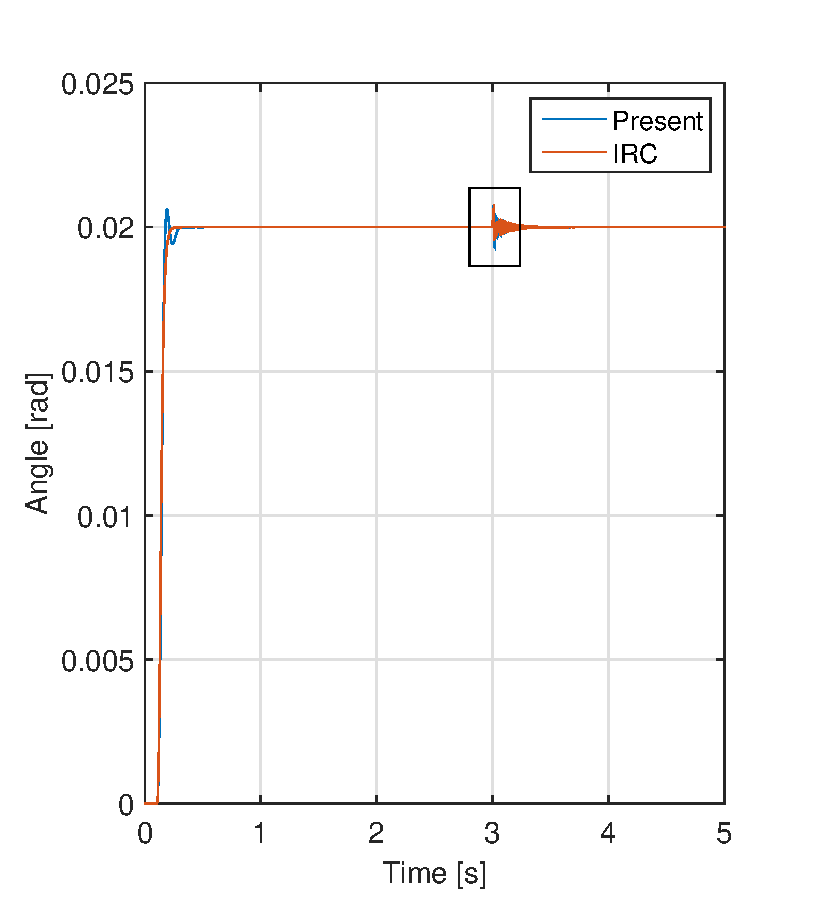
\includegraphics[width=0.46\textwidth, trim=0cm 0cm 1cm 0cm, clip=true]{fig/matlab/irc_dist_input.eps}}
  \qquad
  \subfloat[][\label{fig:irc_dist_input_zoom}Zoom in on disturbance]{
  \includegraphics[width=0.46\textwidth, trim=0cm 0cm 1cm 0cm, clip=true]{fig/matlab/irc_dist_input_zoom.eps}}
  \caption{\label{fig:irc_dist_input} Shows how well the controller attenuates a disturbance impulse (amplitude of $5.1 \times 10^{-3}$) added to the input signal at $t=3s$. The whole step response is shown in (a) with a zoom in on the disturbance in (b).}
\end{figure}

The \abbrIRC capability of rejecting disturbances on the output signal is shown in Figure~\ref{fig:irc_dist_output}. Since the impulse is added directly on the output the steps response peaks accordingly at $t=3s$. It is hard to tell from Figure~\ref{fig:irc_dist_output_zoom}, but the peak is visible for both of the control approaches. After the peak, the methods perform similarly, with a slightly higher damping and amplitude for the \abbrIRC oscillations shown in the zoom in.

\begin{figure}[h!]
  \centering %crop: left bottom right top
  \subfloat[][\label{fig:irc_dist_output_step}Step response]{
  \includegraphics[width=0.46\textwidth, trim=0cm 0cm 1cm 0cm, clip=true]{fig/matlab/distrej_meas.eps}}
  \qquad
  \subfloat[][\label{fig:irc_dist_output_zoom}Zoom in on disturbance]{
  \includegraphics[width=0.46\textwidth, trim=0cm 0cm 1cm 0cm, clip=true]{fig/matlab/distrej_meas_zoom.eps}}
  \caption{\label{fig:irc_dist_output} Shows how well the controller attenuates a disturbance impulse (amplitude of $5.1 \times 10^{-3}$) added to the output signal at $t=3s$. The whole step response is shown in (a) with a zoom in on the disturbance in (b).}
\end{figure}
\FloatBarrier
To further verify the controller capability of handling disturbances with various frequencies, a white noise was added to the input and output signal of the rotational stage ($G$), illustrated in Figure~\ref{fig:irc_int} as $d_i$ and $d_o$, respectively. The \abbrFFT was then performed on the output ($y$) to verify the disturbance rejection for all frequencies, and the result is presented in Figure~\ref{fig:fft_in} and Figure~\ref{fig:fft_out}.

\begin{figure}[h!]
  \centering
  \includegraphics[width=0.7\textwidth]{fig/matlab/whitenoiseoutput.eps}
  \caption{\label{fig:fft_in} The \abbrFFT of the output signal for the \abbrIRC and the present approach, when applying a white noise to the input of G}
\end{figure}

\begin{figure}[h!]
  \centering
  \includegraphics[width=0.7\textwidth]{fig/matlab/whitenoiseinput.eps}
  \caption{\label{fig:fft_out} The \abbrFFT of the output signal for the \abbrIRC and the present approach, when applying a white noise to the output of G}
\end{figure}


The standard deviations of the output signal with a disturbance with $\sigma$ = \unit{1.41\micro\radian} added to both the output and input for the \abbrIRC and the present approach are summarized in Table~\ref{tab:std}.

\begin{table}[h!]
  \centering
  \begin{tabular}{| l | l | l |}
    \hline
    Disturbance applied to: & input & output \\ \hline
      $\sigma_{Present}$ [\unit{\micro\radian}] & $0.68 $ & $1.43$ \\
      $\sigma_{IRC}$ [\unit{\micro\radian}] & $0.45$  & $ 1.46$ \\
    \hline
  \end{tabular}
  \caption{\label{tab:std} Standard deviations of the output signal}
\end{table}

Since the \abbrIRC closed loop bandwidth is a lot higher than the present controller, it is expected that the \abbrIRC is more sensitive to measurement noise and to model errors in terms of stability. Both approaches uses a static notch filter to cancel higher order harmonics, which makes the cancellation sensitive for model changes in the higher resonances. Both make it interesting to see how robust the controller are to model changes in the higher frequencies. A disturbance rejection test was performed on the systems showed in Figure~\ref{fig:high_model_error}, where the highest resonance peak has been moved 83Hz and 97Hz, respectively. An impulse was applied to the output and the resulting response is presented in Figure~\ref{fig:model_dist_high_order}. The \abbrIRC is clearly more sensitive to model errors and becomes unstable when the highest resonance peak has moved by 97Hz.

\begin{figure}[h!]
  \centering
  \includegraphics[width=0.65\textwidth]{fig/matlab/bode_high_model_error.eps}
  \caption{\label{fig:high_model_error} The \abbrFFT of the output signal for the \abbrIRC and the present approach, when applying a white noise to the output of G}
\end{figure}

\begin{figure}[h!]
  \centering %crop: left bottom right top
  \subfloat[][\label{fig:model_83}Model change of 83hz]{
  \includegraphics[width=0.46\textwidth, trim=0cm 0cm 1cm 0cm, clip=true]{fig/matlab/model_high_83hz.eps}}
  \qquad
  \subfloat[][\label{fig:model_97}Model change of 97hz]{
  \includegraphics[width=0.46\textwidth, trim=0cm 0cm 1cm 0cm, clip=true]{fig/matlab/model_high_97hz.eps}}
  \caption{\label{fig:model_dist_high_order} Shows how the controller attenuates a disturbance impulse (amplitude of $5.1 \times 10^{-3}$) added to the output signal at $t=0.1s$. The highest resonance peak of G has in (a) been moved by 83Hz and in (b) by 97Hz.}
\end{figure}

\newpage
\FloatBarrier
\section{Harmonic Cancellation}
The investigated harmonic cancellation methods aims to eliminate disturbances introduced by the linear axis movement. The setup described in \ref{sec:setup} was used to acquire data that later was used for disturbance identification and as a disturbance source for realistic benchmark tests. The yaw angle was acquired in open loop during a linear axis movement corresponding to 50 steps of the stepping motor. The movement was performed with four different speeds (1, 2, 5 and 10 steps/s) around the operating point on the linear axis, which is 3 mm out from the inner position with respect to the beam.

\subsection{Feedforward Disturbance Cancellation}\label{sec:hc}
The acquired stepping voltage and yaw angle was used with the theory in Section~\ref{subsec:distff} to simulate disturbance cancellation using a feedforward approach. The chosen linear speeds in the data acquisition were relatively low compared to normal operation, but used for the purpose of getting enough time between each step in order for each step response to have sufficient time to settle. Figure~\ref{fig:stepinout} shows the yaw angle response from one stepping-motor step and the impulse used as input for the identification of the disturbance model.

\begin{figure}[h!]
  \centering %crop: left bottom right top
  \subfloat[][Impulse used as input signal]{
  \includegraphics[width=0.46\textwidth, trim=0cm 0cm 1cm 0cm, clip=true]{fig/matlab/ff_impulse.eps}}
  \qquad
  \subfloat[][\label{fig:stepout}Impulse response from one step]{
  \includegraphics[ width=0.46\textwidth, trim=0cm 0cm 1cm 0cm, clip=true]{fig/matlab/yaw_angle_mean_1_step_s.eps}}
  \caption{\label{fig:stepinout} Shows the input signal (a) and the mean of 50 time-synchronized acquired step responses (b) at a movement of 1 step/s.}
\end{figure}

The empirical estimate of the disturbance model $P_d$ is obtained by dividing the \abbrFFT of (b) with the \abbrFFT of (a) in Figure~\ref{fig:stepinout}. The resulting empirical estimate is shown for different positions and speeds in Figure~\ref{fig:fft0_3} and \ref{fig:fft_6_5} .

\begin{figure}[h!]
  \centering %crop: left bottom right top
  \subfloat[][\abbrFFT at 0V ]{
  \includegraphics[width=0.46\textwidth, trim=0cm 0cm 0.9cm 0cm, clip=true]{fig/matlab/fft_mean_in_out_0V.eps}}
  \qquad
  \subfloat[][\abbrFFT at 3.25V]{
  \includegraphics[width=0.46\textwidth, trim=0cm 0cm 0.9cm 0cm, clip=true]{fig/matlab/fft_mean_in_out_3V.eps}}
  \caption{\label{fig:fft0_3} \abbrFFT of the response divided by the \abbrFFT of the impulse at two different positions, 0V - 0mrad (a) and 3.25 - 40mrad (b) with different speeds.}
\end{figure}

\begin{figure}[h!]
  \centering %crop: left bottom right top
  \subfloat[][\label{fig:fft_6_5}\abbrFFT at 6.5V]{
  \includegraphics[width=0.46\textwidth, trim=0cm 0cm 1cm 0cm, clip=true]{fig/matlab/fft_mean_in_out_6_5V.eps}}
  \qquad
  \subfloat[][\label{fig:distmodelfit}Identified model]{
  \includegraphics[width=0.46\textwidth, trim=0cm 0cm 1cm 0cm, clip=true]{fig/matlab/model_fit_1step_s.eps}}
  \caption{\label{fig:fft_6_5_modelfit} Shows the \abbrFFT of the response divided by the \abbrFFT at 6.5V - 80mrad (a) at different speeds and the corresponding identified model (b).}
\end{figure}

As seen in the figures, the disturbance model has clear resonance peaks at around 220, 445, 670 and 890Hz. The resonance peak for a specific speed is a multiple of the stepping rate as seen in Figure~\ref{fig:3vzoomin}.

\begin{figure}[h!]
  \centering
  \includegraphics[width=0.7\textwidth]{fig/matlab/fft_mean_in_out_3V_zoomin.eps}
  \caption{\label{fig:3vzoomin} Zoom in on the first resonance peak on the \abbrFFT performed on the data originating from the 3.25 - 40mrad. The resonance peaks are clearly multiples of the stepping rate.}
\end{figure}
\FloatBarrier
Figure~\ref{fig:fft_6_5_modelfit} shows the identified model for the data acquired at 6.5V and 1 step/s. In order to sufficiently model four resonances, a 19 zeros and 20 poles transfer function was needed. The model is sufficient for simulations but have to be reduced for a reasonable implementation in terms of computational efficiency. The identification was performed using Matlab System Identification Toolbox with a selected frequency focus from 30-1000Hz. The identified disturbance model $P_d$ is presented in its final form in Appendix~\ref{cha:definition}. $K_f$ was calculated as $K_f=P_d/G$.
The disturbance model was benchmarked with 2 slightly different disturbances, first with the mean shown in Figure~\ref{fig:stepout} (the signal used in the identification) and then with a signal picked out as one period from the original acquired data. The disturbance rejection results at 6.5V and 1 step/s can be seen in Figure~\ref{fig:benchmark_dist}. The feedforward of the modeled disturbance manages to mitigate the disturbance on the yaw angle by almost half of the amplitude, when the mean is fed as disturbance. However, with the more realistic disturbance, the disturbance on the yaw angle is at first amplified by almost the double but settles quickly after that to a level below the level of the controller without disturbance feedforward.

\begin{figure}[h!]
  \centering %crop: left bottom right top
  \subfloat[][Mean as disturbance]{
  \includegraphics[width=0.46\textwidth, trim=0cm 0cm 1cm 0cm, clip=true]{fig/matlab/cancellation_1_step_s.eps}}
  \qquad
  \subfloat[][Original acquired signal as disturbance ]{
  \includegraphics[width=0.46\textwidth, trim=0cm 0cm 1cm 0cm, clip=true]{fig/matlab/cancellation_1_step_s_real_dist.eps}}
  \caption{\label{fig:benchmark_dist} Shows the effect of the feedforward disturbance cancellation with the mean of the acquired response added as disturbance (a) and one period of the acquired response added as disturbance (b).}
\end{figure}
\FloatBarrier
To illustrate the model efficiency with different step rates, a benchmark test with the same identified model as above was performed with the mean corresponding to each of the stepping rates added as disturbance. The outcome is presented in Table~\ref{tab:std_diff_speed} as the standard deviation of the yaw angle, showing that a single model is sufficient to reduce the disturbance level for several other stepping rates as well.

\begin{table}[h!]
  \centering
  \begin{tabular}{| l | l | l | l | l |}
    \hline
      Speed & 1 step/s & 2 step/s & 5 step/s & 10 step/s\\ \hline
      $\sigma_{Present}$ & 2.15 & 2.23 & 3.90 & 3.76\\
      $\sigma_{Present + dist.FF.}$ & 1.19 & 2.04 & 2.06 & 2.59\\
    \hline
  \end{tabular}
  \caption{\label{tab:std_diff_speed} Standard deviations of the output with and without disturbance feedforward for the different speeds with the mean of the acquired response corresponding to each speed added as disturbance. The model used in the disturbance feedforward was identified from the 6.5V and 1step/s data.}
\end{table}

\FloatBarrier
To benchmark how well the cancellation works with model errors, a simulation with 4 different perturbed models were performed with the disturbance feedforward tuned as before. The models including the original system itself is shown in Figure~\ref{fig:hc_me_bode}, where the first resonance peak has been perturbed. This models the previous identified behavior when the rotaional stage rotates from 0 to 20mrad.

\begin{figure}[h!]
  \centering
  \includegraphics[width=0.7\textwidth]{fig/matlab/bode_rfdc_modelerror.eps}
  \caption{\label{fig:hc_me_bode} Bode diagram of the 5 different models used for the simulation of model error, including the original model G - 38.1Hz.}
\end{figure}

The \abbrFFT of the simulation results can be seen in Figure~\ref{fig:hc_model_error}. The attenuation of the disturbance's major frequency is shown in (a) which shows that the cancellation is still efficient even with model errors being present. The original controller and system without disturbance cancellation is included in the plots as a reference and is named \emph{Present - 38.1 Hz}. The plot in (b) illustrates the impact that the model errors have to the attenuation of some other resonances present in the system. Here 130Hz is choosen as an example to illustrate that the cancellation with model errors can lead to amplification at some frequencies.


\begin{figure}[h!]
  \centering %crop: left bottom right top
  \subfloat[][Attenuation of major frequency]{
  \includegraphics[width=0.46\textwidth, trim=0cm 0cm 1cm 0cm, clip=true]{fig/matlab/hc_model_error.eps}}
  \qquad
  \subfloat[][Impact on 92.3Hz component]{
  \includegraphics[width=0.46\textwidth, trim=0cm 0cm 1cm 0cm, clip=true]{fig/matlab/hc_model_error92.eps}}
  \caption{\label{fig:hc_model_error} Disturbance cancellation effectiveness with model errors. The attenuation of the major frequency is shown in (a) while the attenuation of the 130Hz component is shown in (b).}
\end{figure}


\FloatBarrier
\subsection{Cancellation with Internal Model Principle}
The implementation of the \abbrIMP cancellation method was based on the theory in Section~\ref{subsec:distimp}. A pure sinusoidal disturbance has the generating polynomial $\Gamma(s) = s^2 = + w^2$, where the selected frequency to reject was  $w = 2\pi50$. This choice of polynomial gives full attenuation in the selected frequency but impacts on the attenuation of the 38.1 Hz resonance peak. Hence, in order to get sufficient attenuation in both of the frequencies a damping coefficient was added to the polynomial. The normalized continuous transfer function that was discretized and added to the system is presented below.

\begin{equation}
  C_{imp}(s) = \frac{(2pi50)^2}{s^2 + s + (2pi50)^2}
\end{equation}

The controller, shown in its full in \eqref{eq:imp_c}, was tuned using Matlabs's SISO-tool aiming to achieve equivalent performance as the present controller. The controller was based on a PI-controller with a notch filter to damp out higher order frequencies modes and a complex pair of zeros placed between the resonance peaks 38.1 and 50Hz to gain some phase margin. Finally, a lead-filter was added to increase the phase margin even more.

\begin{equation}
  \label{eq:imp_c}
  C(s) = \frac{25.33z^7 - 130.6z^6 + 301.9z^5 - 429z^4 + 424.7z^3 - 291.5z^2 + 121.8z - 22.64}{z^7 - 3.6z^6 + 5.4z^5 - 4.5z^4 + 2.2z^3 - 0.63z^2 + 0.096z - 0.0061}
\end{equation}




Figure~\ref{fig:rfdc_s_gc} shows the resulting closed loop system and the sensitivity function from output disturbance to system output. The 2 drops in 38.1 and 50 Hz is clearly visible in the sensitivity function, but note that the attenuation of the 38.1 Hz is a bit less for the \abbrIMP approach. This phenonoma is sometimes called the \emph{waterbed effect} meaning that if sensitivity to a disturbance is suppressed at one frequency it will increase in some other.

\begin{figure}[h!]
  \centering %crop: left bottom right top
  \subfloat[][Closed loop system]{
  \includegraphics[width=0.46\textwidth, trim=0cm 0cm 1cm 0cm, clip=true]{fig/matlab/gc_imp.eps}}
  \qquad
  \subfloat[][Sensitivity function]{
  \includegraphics[width=0.46\textwidth, trim=0cm 0cm 1cm 0cm, clip=true]{fig/matlab/s_imp.eps}}
  \caption{\label{fig:rfdc_s_gc} Closed loop system (a) and sensitivity function, the transfer function from output disturbance to system output (b).}
\end{figure}

\FloatBarrier
The \abbrIMP method was benchmarked against the present controller in all tests. As a proof of concept, a 50Hz sinusoidal disturbance was added as a disturbance and the attenuation (in the perfect case) can be seen in Figure~\ref{fig:rfdc_p_atten}. The \abbrIMP managed to attenuate 96\% of the added disturbance. The missing 4 percent can be explained by the addition of damping that was added to the generating polynomial.

\begin{figure}[h!]
  \centering %crop: left bottom right top
  \subfloat[][Time domain]{
  \includegraphics[width=0.46\textwidth, trim=0cm 0cm 1cm 0cm, clip=true]{fig/matlab/distrej.eps}}
  \qquad
  \subfloat[][\abbrFFT]{
  \includegraphics[width=0.46\textwidth, trim=0cm 0cm 1cm 0cm, clip=true]{fig/matlab/distrej_fft.eps}}
  \caption{\label{fig:rfdc_p_atten} The time response is shown in (a) with cancellation of 50Hz component. The \abbrFFT performed on (a) after the response had settled is shown in (b).}
\end{figure}

For a more realistic benchmark test, disturbance data collected at 10 steps/s was added to the output of the system. The result is presented in Figure~\ref{fig:imp_realdata} where it is clear that the 50Hz component has been damped out efficiently.

\begin{figure}[h!]
  \centering
  \includegraphics[width=0.7\textwidth]{fig/matlab/distrej_realstep_fft.eps}
  \caption{\label{fig:imp_realdata} \abbrFFT performed on the output signal after the response had settled, with the acquired data as input signal.}
\end{figure}

\newpage~\newpage~
\FloatBarrier
Finally, the cancellation approach was tested for model robustness following the procedure described in Section~\ref{sec:hc}. The perturbed models used in the simulation can be seen in Figure~\ref{fig:hc_me_bode}. The attenuation of the selected frequency is presented in Figure~\ref{fig:imp_model_error1} showing that the cancellation is efficient for major model errors. One main drawback with this approach is depicted in Figure~\ref{fig:imp_model_error2} where the 130Hz component has been amplified due to the addition of the \abbrIMP cancellation strategy.


\begin{figure}[h!]
  \centering %crop: left bottom right top
  \subfloat[][\label{fig:imp_model_error1}Attenuation of selected frequency]{
  \includegraphics[width=0.46\textwidth, trim=0cm 0cm 1cm 0cm, clip=true]{fig/matlab/imp_model_error_real50.eps}}
  \qquad
  \subfloat[][\label{fig:imp_model_error2}Impact on 130Hz component]{
  \includegraphics[width=0.46\textwidth, trim=0cm 0cm 1cm 0cm, clip=true]{fig/matlab/imp_model_error_real.eps}}
  \caption{\label{fig:imp_model_error}  Disturbance cancellation effectiveness with model errors. The attenuation of the major frequency is shown in (a) while the attenuation of the 130Hz component is shown in (b).}
\end{figure}

\newpage
\FloatBarrier
\subsection{Repetitive Feedforward Disturbance Cancellation}
The Repetitive Feedforward Disturbance Cancellation (\abbrRFDC) method was implemented to reject three known disturbances. Hence, three second order disturbance models as given in \eqref{eq:sinm} were augmented as shown in \eqref{eq:augmentedres}. The chosen frequencies for cancellation were $w_1 = 2\pi60$, $w_2 = 2\pi90$ and $w_3 = 2\pi200$ rad/s.

\begin{subequations}
  \label{eq:augmentedres}
  \begin{alignat}{2}
    & \mathbf{A_{de}} = diag
    \begin{pmatrix}
      \begin{bmatrix}
         0 & 1\\[0.3em]
         -w_1^2 & 0
       \end{bmatrix}  &
       \begin{bmatrix}
          0 & 1\\[0.3em]
          -w_2^2 & 0
        \end{bmatrix} &
        \begin{bmatrix}
          0 & 1\\[0.3em]
          -w_3^2 & 0
        \end{bmatrix} \\
      \end{pmatrix} \\
    & \mathbf{C_{de}} =
        \begin{bmatrix}
            1 & 0 & 1 & 0 & 1 & 0 \\
        \end{bmatrix}
  \end{alignat}
\end{subequations}

These equations where augmented according to \eqref{eq:augumented} with the discrete time system matrices which can be seen in its full form in Appendix~\ref{cha:definition}. The observer was implemented in state space form, with the following equations.

\begin{subequations}
\label{eq:augmented}
  \begin{alignat}{2}
    & \mathbf{A_{obs}} = \mathbf{A - KC} \\
    & \mathbf{B_{obs}} = \mathbf{[B, K]}^T \\
    & \mathbf{C_{obs}} = diag(\mathbf{C_{zs}, C_{zd}, C_{zd}, C_{zd}}) \\
    & \mathbf{D_{obs}} = zeros(4,2)
  \end{alignat}
\end{subequations}


A sufficient gain $K$ was calculated by using Kalman (\texttt{dlqe} in Matlab), with a high measurement (R) to process noise (Q) ratio, trusting in the predefined model. The values provided to the \texttt{dlqe} function are listed in \ref{tab:kalman}.

\begin{table}[h!]
  \centering
  \begin{tabular}{| l | l |}
    \hline
    Parameter & Value \\ \hline
    $R$ & $1$ \\
    $Q$ & $10^{-5}$ \\
    $G$ & $[1, 0, 0, 0, 0, 0, 10, 0, 8, 0, 70, 0]^T$ \\
    \hline
  \end{tabular}
  \caption{\label{tab:kalman} Parameters used for calculating the observer gain.}
\end{table}

The \abbrRFDC method was benchmarked against the present controller in all tests. As a proof of concept, three sinusoidal disturbances with frequencies $w_1$, $w_2$ and $w_3$ were added to the output of the system. Even though all of them were observed only $w_3$ was feedforwarded to cancel out the 200Hz component to begin with. The result is shown in Figure~\ref{fig:1_dist_both}, where it is clear that the 200Hz disturbance is perfectly canceled by the feedforward algorithm. Since 200Hz is a multiple of the sampling frequency $F_s = 2000Hz$, one period is sufficient to capture a full number of periods within the switching times. The switch was set to turn on (load on period) at $t_{on}=2s$ and to turn off at $t_{off}=2+1/200s$, which was the time when all the observed estimates had converged.

To prove the concept for multiple harmonic cancellation, all three of the estimated disturbances were added and subtracted from the input. To capture an even number of cycles, the switching times for the 60Hz an 90Hz were set to [$t_{on}=2s, t_{off}=2+6/60 s$] and [$t_{on}=2s, t_{off}=2+9/90 s$], respectively.

\begin{figure}[h!]
  \centering %crop: left bottom right top
  \subfloat[][\label{fig:1_dist} Time domain]{
  \includegraphics[width=0.46\textwidth, trim=0cm 0cm 1cm 0cm, clip=true]{fig/matlab/1_dist.eps}}
  \qquad
  \subfloat[][\label{fig:1_dist_fft} \abbrFFT]{
  \includegraphics[width=0.46\textwidth, trim=0cm 0cm 1cm 0cm, clip=true]{fig/matlab/1_dist_fft.eps}}
  \caption{\label{fig:1_dist_both} The time response is shown in (a) with cancellation of 200Hz after 2s. The \abbrFFT of (a) from t=2.5s to t=5s is shown in (b).}
\end{figure}

\begin{figure}[h!]
  \centering %crop: left bottom right top
  \subfloat[][\label{fig:3_dist} Time domain]{
  \includegraphics[width=0.46\textwidth, trim=0cm 0cm 1cm 0cm, clip=true]{fig/matlab/3_dist.eps}}
  \qquad
  \subfloat[][\label{fig:3_dist_fft} \abbrFFT]{
  \includegraphics[width=0.46\textwidth, trim=0cm 0cm 1cm 0cm, clip=true]{fig/matlab/3_dist_fft.eps}}
  \caption{\label{fig:3_dist_both} The time response is shown in (a) with cancellation of 60, 90 and 200Hz after 2s. The \abbrFFT of (a) from t=2.5s to t=5s is shown in (b).}
\end{figure}

The result is presented in Figure~\ref{fig:3_dist_both}, which also illustrates a perfect cancellation. Note that the \abbrFFT analysis is performed on data from t=2.5 to t=5s i.e. at the time when the feedforward cancellation has been added and the response has settled.

For a more realistic benchmark test, disturbance data collected at 10 steps/s was added to the output of the system. $w_1$, $w_2$ and $w_3$ are all major components of the acquired disturbance so the model in the observer were kept the same as before. The result presented in linear scale is shown in Figure~\ref{fig:fft_linear} where it is clear that modeled frequencies have been damped out efficiently. The gain of the 60Hz component for instance, is with the \abbrRFDC reduced to more than 1/8 of its original amplitude.

\begin{figure}[h!]
  \centering
  \includegraphics[width=0.7\textwidth]{fig/matlab/3real_dist_fft.eps}
  \caption{\label{fig:fft_linear} \abbrFFT of the added perturbation with and without cancellation of the 60Hz, 90Hz and the 200Hz component.}
\end{figure}

A converging time of 2 seconds might be considered as fairly high. Increasing the gain in G in Table~\ref{tab:kalman} would lead to a quicker convergence but would also imply in more noise added to the observed model, especially for high frequency models with frequencies close to the Nyquist frequency. This phenomenon is illustrated in Figure~\ref{fig:ph_lowgain} and \ref{fig:ph_highgain}, where the value of G for the 200Hz model was increased 7 times. Figure~\ref{fig:ph_lowgain} shows a clean representation in the frequency domain with a settling time longer than 5 seconds, Figure~\ref{fig:ph_highgain} shows a settling time around 2 seconds but with a less clean representation in the frequency domain.

\begin{figure}[h!]
  \centering %crop: left bottom right top
  \subfloat[][Time domain]{
  \includegraphics[width=0.46\textwidth, trim=0cm 0cm 1cm 0cm, clip=true]{fig/matlab/model_conv.eps}}
  \qquad
  \subfloat[][\abbrFFT]{
  \includegraphics[width=0.46\textwidth, trim=0cm 0cm 1cm 0cm, clip=true]{fig/matlab/model_conv_fft.eps}}
  \caption{\label{fig:ph_lowgain} Shows the convergence (a) of the 200Hz observed harmonic with $G = [1, 0, 0, 0, 0, 0, 10, 0, 8, 0, 10, 0]^T$. The \abbrFFT of (a) is shown in (b), showing a clean model of the 200 Hz component.}
\end{figure}

\begin{figure}[h!]
  \centering %crop: left bottom right top
  \subfloat[][Time domain]{
  \includegraphics[width=0.46\textwidth, trim=0cm 0cm 1cm 0cm, clip=true]{fig/matlab/model_conv_w.eps}}
  \qquad
  \subfloat[][\abbrFFT]{
  \includegraphics[width=0.46\textwidth, trim=0cm 0cm 1cm 0cm, clip=true]{fig/matlab/model_conv_fft_w.eps}}
  \caption{\label{fig:ph_highgain} Shows the convergence (a) of the 200Hz observed harmonic with $G = [1, 0, 0, 0, 0, 0, 10, 0, 8, 0, 70, 0]^T$. The \abbrFFT of (a) is shown in (b), including a lot of other frequency components in the 200 Hz harmonic model.}
\end{figure}

\FloatBarrier
An even higher gain would lead to a more noise added to the model and a reduction in cancellation performance which is illustrated in Figure~\ref{fig:convergence}, where it is clear that a shorter converge time implies in a reduction in cancellation performance. The figures show the cancellation of the 200Hz component with a converge time of 2s in (a) achieved with a gain of 70 as before and a converge time of 1s in (b) achieved with a gain of 140.

\begin{figure}[h!]
  \centering %crop: left bottom right top
  \subfloat[][Converged within 2s]{
  \includegraphics[width=0.46\textwidth, trim=0cm 0cm 1cm 0cm, clip=true]{fig/matlab/converge70.eps}}
  \qquad
  \subfloat[][Converged within 1s]{
  \includegraphics[width=0.46\textwidth, trim=0cm 0cm 1cm 0cm, clip=true]{fig/matlab/converge140.eps}}
  \caption{\label{fig:convergence} Shows the cancellation performance for 200Hz with a model state convergence of 2s in (a) and 1s in (b).}
\end{figure}

To overcome this issue, a bandpass filter for the selected frequency could be added to reduce the noise level of the model and thereby enabling for quicker convergence. However, this filter needs have zero-phase, at least for the selected frequencies, making the range of applicable filters much more narrow. One example of bandpass filter could be

\begin{equation}
  BP = k\frac{s^2 + 2\xi_aws + w^2}{s^2 + 2\xi_bws + w^2}
\end{equation}

where $k=1/100$, $\xi_a=1$ and $\xi_b=0.01$, which has zero phase shift for signals entering at 200Hz, but shifts all other frequencies. Tests where performed with this filter but without any increase in disturbance cancellation performance, this might be due to numerical problems that origin from an insufficient sampling rate.

To benchmark the sensitivity to model errors, a similar simulation as in Section~\ref{sec:hc} was performed on the \abbrRFDC method. The perturbed models used in the simulation can be seen in Figure~\ref{fig:hc_me_bode}. The attenuation of the selected frequency is shown in Figure~\ref{fig:rfdc_model_error1} showing that the cancellation is efficient with low model errors, but amplifies the component if the error is too large (\abbrRFDC - 43.4 Hz in figure). The plot in Figure~\ref{fig:rfdc_model_error2} illustrates that the \abbrRFDC is not amplifying other major frequencies components by showing the 130 Hz component.

\begin{figure}[h!]
  \centering %crop: left bottom right top
  \subfloat[][\label{fig:rfdc_model_error1} Attenuation of selected frequency]{
  \includegraphics[width=0.46\textwidth, trim=0cm 0cm 1cm 0cm, clip=true]{fig/matlab/rfdc_model_error_real60.eps}}
  \qquad
  \subfloat[][\label{fig:rfdc_model_error2} Impact on 130Hz component]{
  \includegraphics[width=0.46\textwidth, trim=0cm 0cm 1cm 0cm, clip=true]{fig/matlab/rfdc_model_error_real.eps}}
  \caption{\label{fig:rfdc_model_error} Disturbance cancellation effectiveness with model errors. The attenuation of the major frequency is shown in (a) while the attenuation of the 130Hz component is shown in (b).}
\end{figure}

\newpage
\FloatBarrier
\section{Comparison}
This section compares and summarizes the stand-alone control approaches (\abbrIRC and \abbrMRACPE) and the approaches that aims to cancel harmonics (\abbrFDC, \abbrRFDC and \abbrIMP). Table~\ref{tab:comp_h} and \ref{tab:comp} summarizes comparable results presented in the previous sections. Key values from the graphs have been collected to give the reader an overview of the achieved performance for each control approach.

In Table~\ref{tab:comp_h}, the cancellation effectiveness is measured as attenuation of the resonance peak with respect to the present approach. For aspect nr 3 and 4, the attenuation is measured with respect to the present controller that also includes the perturbed model written in the parentheses.

\begin{table}[h!]
  \centering
  \begin{tabular}{| l | P{3.7cm} | P{2.2cm} | P{2.2cm} | P{2.2cm} |}
    \hline
      \bf{Nr} & \bf{Aspect} & \bf{\abbrFDC} & \bf{\abbrRFDC} & \bf{\abbrIMP} \\ \hline
    1 & Affecting closed loop system & No & No & Yes\\ \hline
    2 & Cancellation effectiveness of major frequency, attenuation-[\%]                & 64.6 & 88.4 & 83.3\\ \hline
    3 & Cancellation with model errors (model's 1st resonance at 28.2Hz), attenuation-[\%] & 40.5 & 26.6 & 73.5\\ \hline
    4 & Cancellation with model errors (model's 1st resonance at 43.4Hz), attenuation-[\%] & 57.7 & 5.0 & 83.4\\ \hline
    5 & Implementation considerations & Requires high order model, computational demanding. & Requires observer, computational demanding. Can be used as add-on.& Controller must be retuned 6 when selecting another frequency. \\ \hline
  \end{tabular}
  \caption{\label{tab:comp_h} Key parameters for the harmonic cancellation control approaches.}
\end{table}

In Table~\ref{tab:comp}, the closed-loop bandwidth is presented for each approach, where "-" means that a theoretical bandwidth is missing for the \abbrMRACPE. The tracking error is presented as the standard deviation of the difference between reference and output signal, taken after each approach has settled. The tracking error with model errors being present is shown in nr 4-7. Here, infinite tracking error means that the system is unstable. First resonance peak frequencies are selected to put the system on the border of instability. Nr 7 presents the disturbance rejection with a disturbance added to the system output, measured in settling time from that the disturbance was added.

\begin{table}[h!]
  \centering
  \begin{tabular}{| l | P{3.4cm} | P{2.2cm} | P{2.2cm} | P{2.8cm} |}
    \hline
    \bf{Nr} & \bf{Aspect}  & \bf{Present} & \bf{\abbrIRC} & \bf{\abbrMRACPE} \\ \hline
    1 & Closed-loop Bandwidth [Hz] & 9.7 & 73.3 & -\\ \hline
    2 & Gain/Phase margin [dB / $^{\circ}$] & 14.4/66.2 & 13.1/49.4 & -\\ \hline
    3 & Tracking error, periodic input $\sigma$-[mrads] & $0.29$ & $0.03$ & $0.11$\\ \hline
    4 & Tracking error with model errors (model's 1st resonance at 22.0Hz), $\sigma$-[mrads] & $\infty$ & 0.03 & 0.21\\ \hline
    5 & Tracking error with model errors (model's 1st resonance at 67.2Hz), $\sigma$-[mrads] & $\infty$ & 0.03 & 0.11\\ \hline
    6 & Tracking error with model errors (model's 1st resonance at 17.6Hz), $\sigma$-[mrads] & $\infty$ & $\infty$ & 0.47\\ \hline
    7 & Tracking error with model errors (model's 1st resonance at 77.7Hz), $\sigma$-[mrads] & $\infty$ & $\infty$ & 0.11\\ \hline
    8 & Output disturbance rejection, settling time (1\%) [ms] & 8 & 25 & 260\\ \hline
    9 & Input/Output disturbance rejection, $\sigma$-[\unit{\micro\radian}] & $0.68 $/$1.43$ & $0.45$/$1.46$ & $1.95$/$1.41$\\ \hline
    10 & Stability issues & Unstable with high model errors & Unstable with high model errors, but better than present & Good adaption even with model errors, but tuning for quicker adaption easily leads to instability.  Stability only proven in continuous time. \\ \hline
    11 & Design and implementation considerations & Straight- forward technique, allowing for basic stability analysis & Same as present & Hard to tune. High computational burden for higher order models.\\ \hline
  \end{tabular}
  \caption{\label{tab:comp} Key parameters for the stand-alone control approaches.}
\end{table}

%Sätt av ett kort kapitel sist i rapporten till att avrunda och föreslå rikningar för framtida utveckling av arbetet.
% !TEX root = main.tex
\chapter{Conclusions and Future work}\label{cha:conclusion}

\section{Conclusions}

As seen in the zoom-in, the \abbrIRC is slightly more damped but has a high frequency ringing in 448Hz, the same frequency as the model's second resonance peak. In reality it would be plenty of  higher resonance (all are not modeled) that will lead to more ringing and bad disturbance rejection.

\section{Future work}

To achieve intersample disturbance rejection, a multi rate control technique with a control period shorter than the sampling rate can be implemented, as proposed in \citep{fujimoto2009rro}. However if


% THESIS PLAN
% % !TEX root = main.tex
%en preliminär problemformulering satt i relation till litteraturbasen
\chapter{Introduction}\label{cha:intro}

\section{Background}
The piezoelectric effect is a phenomenon that arises in certain solid materials when an electric potential is generated in response to applied mechanical stress. The effect was first discovered by Jacques and Pierre Curie in 1880 when they found that applying pressure to a quarz crystal generates electrical potential. Today, the effect is commonly encountered in daily life and utilized in for example lighters, buzzers and loudspeakers.

Smart materials such as piezoelectric and magnetostrictive materials are nowadays commonly used in precision actuators due to their ability to convert electrical energy into mechanical energy. Piezoelectric materials have been commercially available for almost 45 years and have become indispensable for the nanopositioning industry \citep{Piezo:2008}. In cases where a relatively small displacement range is required (travel ranges up to \unit{500}{\micro\meter}) a piezo electric device is the actuator of choice due to its fast response, high resolution and its ability to generate large mechanical forces for small amounts of power in compact designs \citep{SurveyOfControlIssues:2007}.

High precision positioning systems are vital in e.g. scanning tunneling microscopes (\abbrSTM), atomic force microscopes (\abbrAFM) and in semiconductor lithography. In \abbrAFM, for instance, high precision positioning is required to control the vertical position of the scanning probe to keep the force constant between the sample surface and the probe tip. An topographical image of the sample is obtained by raster-scanning the probe over the sample surface and plotting the vertical displacement against the probe's x-y position. A positioning system that keeps the force constant down to an atomic-scale resolution is thus inevitable in order to obtain a high resolution image without damaging the sample \citep{SurveyOfControlIssues:2007}.

The Equipment Controls and Electronics section in the Engineering Department at \abbrCERN (European Organization for Nuclear Research) is developing a high precision positioning system for the control of a piezo-actuated rotational stage used in the UA9 Crystal Collimation study. The stage uses a piezo electric linear stack actuator to displace a flexible lever arm mechanism which generates the rotational movement.

\section{Purpose and Goal}
Crystalline solids have the ability to constrain the directions that particles take as they pass through, this is commonly called the "channelling" property. The UA9 collaboration at \abbrCERN is investigating how tiny bent crystals can help to steer particle beams in modern hadron colliders such as the Large Hadron Collider (\abbrLHC) \citep{WebsiteUA9:2016}. In high energy colliders, such as the \abbrLHC, particles tends to drift outwards creating a beam halo. These particles surrounding the beam, can be lost and cause damage to sensitive parts in the accelerator. By using bent crystals, halo particles can be efficiently extracted from the beam and collected by absorbers further away, reducing the complexity of the system. One major difficulty that aries is that the higher the energy of the particle, the lower the angular acceptance for channeling. Hence, a high precision positioning mechanism with a high angular accuracy is required. The rotational stage (with a range of \unit{20}{\milli\rad}) is of necessity to be able to track reference trajectories at ramp rates of \unit{100}{\micro\radianpersecond} and reject external disturbances to maintain a maximum tracking error of $\pm$\unit{1}{\micro\rad}.

This project aims to identify the possible control approaches that could be applicable to this problem to achieve the desired performance.

\section{Prospective challenges}
First of all, piezoelectric  actuators show strong nonlinear properties such as hysteresis and creep (drift), which have to be compensated for. Moreover, the mechanical flexural structure in combination with the piezo electric characteristics leads to a highly resonant structure, making it difficult to achieve the desired performance while operating the rotational stage within noisy environments with external disturbances such as ground vibrations.

Furthermore this rotational stage is attached to a linear stage which is composed by a leadscrew, a stepping motor and an axel. The linear movement adds additional perturbation to the rotational stage due to imperfections in the leadscrew and detent torque and stepping nature of the motor.

Finally the system dynamics also show linear position dependence requiring a controller that is robust to such variations.

\section{Related work}
One attempt to achieve the desired performance has already been made. The proposed controller, presented in \citep{ButcherController:2015} delivers reasonable performance but does not fulfill the requirements during movement. The authors proposes a PID controller in combination with a pre-filter, and a hysteresis compensator. The controller has shown high disturbance rejection at the first resonance peak as well as good tracking performance.

\section{Outline}
This thesis plan presents an overview of the thesis, including method, literature base and expected results. The method and work flow of the thesis as well as a comprehensive literature review is given in Chapter~\ref{cha:method}. In Chapter~\ref{cha:result} the results that can be expected half way through the project is discussed while a brief summary of the thesis can be found in Chapter~\ref{cha:conclusion}.

% % !TEX root = main.tex
% en preliminär beskrivning av angreppssätt
\chapter{Method}\label{cha:method}
This thesis will identify possible control approaches that could be applicable to the rotational stage at \abbrCERN in order to meet the performance requirements.
First of all, a brief analysis of the already developed controller will be done in order to point out the drawbacks and determine which controller qualities that have to be improved in order to achieved the desired performance during linear movement of the rotational stage. The main work will then consist of investigating different control approaches such as feedforward, H-infinity, iterative or state feedback control. The most promising approaches will be benchmarked in simulations and compared to the existing algorithm. Finally, the most promising alternative will be implemented and tested on the real rotational stage.

\section{Literature review}
Here follows a review of the preliminary literature base that will be used in this thesis. It will most likely be extended with more articles, papers and books during the work with this thesis.

\subsection*{\citep*{Biggio:2014} {\small \emph{- Memory characteristics of hysteresis and creep in multi-layer piezoelectric actuators: An experimental analysis}}}
The aim of this article is to provide an explanation of peculiar features of the piezoelectric actuator (\abbrPEA) response. It presents an experimental characterization of the nonlinear effects i.e. hysteresis and creep in a \abbrPEA. The authors find that both the instantaneous and delayed response of the PEA have hysteric dependence on the applied voltage level.
Moreover, they present experimental evidence for that the two observed hysteretic relationships share a common memory structure i.e. they are not truly independent nonlinear phenomenas.

\subsection*{\citep*{ButcherIdentification:2015}{\small \emph{- On the identification of Hammerstein systems in the presence of an input hysteretic nonlinearity with nonlocal memory: Piezoelectric actuators – an experimental case study}}}
This paper discusses the identification procedure of the linear dynamic part of piezo based actuators. A Hammerstein structure, consisting of a static (rate independent) hysteresis model with nonlocal memory (the current output does not only depend on the current input voltage but also on its history) and a linear dynamic model, is employed in order to model the hysteretic and dynamic behavior of the actuator.

The authors state that for the identification of the linear part of the actuator, a careful choice of the driving signal has to be made to avoid modifying the characteristics of the excitation. They show that a choice of a \abbrPBRS signal allows the decoupling of the identification of the linear and nonlinear part, since the nonlinear part only transforms the \abbrPBRS signal into another \abbrPBRS.

\subsection*{\citep*{ButcherController:2015} {\small \emph{- Controller Design and Verification for a Rotational Piezo-based Actuator for Accurate Positioning Applications in Noisy Environments}} }
This paper presents the modeling and controller design of a piezo actuated rotational stage operating in a noisy environment at CERN. The authors have adopted a Hammerstein structure, allowing them, in principal, to decouple the nonlinear hysteresis from the linear system dynamics. The extracted linear dynamics is identified as an OE system using several pseudo random binary signals (\abbrPBRS) as excitation signals. By adding different voltage biases to the PBRS it is also verified that the operating voltage point influences the identified transfer function (\abbrTF). The DC gain and the first resonance frequency and amplitude is affected due to the nonlinear piezo properties.

A 2-\abbrDOF controller (feedback and prefilter) and a hysteresis compensator are adopted in order to obtain the desired tracking and disturbance rejection. The proposed controller is designed as a series combination of a \abbrPID controller, a lead network and a 4\textsuperscript{th} order notch filter according to the quantitative feedback theorem (\abbrQFT). The proposed controller is experimentally tested and shows both disturbance rejection and good tracking capability.

\subsection*{\citep*{SurveyOfControlIssues:2007} {\small \emph{- A survey of control issues in nanopositioning}} }
This paper reviews the control-related research in nanopositioning, covering nanopositioning applications, actuators and sensors as well as control challenges. It focuses on piezoelectric actuators discussing both issues in control and different control techniques. Modeling techniques for the nonlinear effects i.e. creep and hysteresis as well as issues such as vibrations and modeling errors are presented in this work. Finally, different control schemes to mitigate the impact from these issues are reviewed such as feedback, forward, iterative and sensor less control.


\subsection*{\citep*{Piezo:2008} {\small \emph{- Piezoelectrics in Positioning, Tutorial on Piezotechnology in Nanopositioning Applications}} }
This tutorial by Physik Instrumente (PI) gives the reader an overview of the fundamentals of piezoelectricity, piezomechanics and piezo actuators as well as detailed information regarding control approaches, environmental dependencies and design of piezoelectric positioning drives/systems. The electrical, mechanical and thermal behavior of piezoelectric actuators is described by basic equations presented in this paper. Several methods to improve the piezo dynamics are also discussed, such as linearization, signal preshaping and InputShaping® which is a patented real-time feedforward technology.

\subsection*{\citep*{FlemingLeang:2014} {\small \emph{- Design, Modeling and Control of Nanopositioning Systems}} }
This book covers the complete design cycle of nanopositioning systems. Some relevant chapters with respect to this thesis are Hysteresis Modeling and Control, Noise in Nanopositioning and Mechanical Design: Flexure-Based Nanopositioners.


\section{Timeplan}
%en tidplan för examensarbetets genomförande inklusive planerade datum för halvtidskontroll och framläggning
Figure~\ref{fig:timeplan} shows the timeplan for the master thesis project. \emph{HP} and \emph{FP} stands for halftime presentation and fulltime presentation, respectively. In addition to the master thesis work, some hardware testing will be carried out from time to time, throughout the whole thesis period.

\begin{figure}[h] %tbp
 \centering %crop: left bottom right top
 \includegraphics[trim=1cm 12cm 5cm 5.5cm, clip=true, scale=0.42]{fig/timeplan}
 \caption{\label{fig:timeplan}%
 Master Thesis timeplan}
 \end{figure}

% % !TEX root = main.tex
%preliminära resultat som kan demonstreras vid halvtidskontroll
\chapter{Result}\label{cha:result}
This section describes future results that could be expected half way through the project.

\section{Control Approaches}
Half way through the project, all control approaches that have been identified should be presented here. Furthermore, all control approaches that at the time have been simulated will be presented with a schematic structure, transfer functions or state space model, a bode plot of the closed loop system and additional plots for illustration of the trajectory tracking capability and the robustness.

\section{Benchmark tests}
Benchmark tests will be carried out on all simulated control approaches and presented here. Comparisons between the new control approaches and the existing algorithm with respect to disturbance rejection, trajectory tracking and closed loop bandwidth will be illustrated in this section with plots and tables.

% %Sätt av ett kort kapitel sist i rapporten till att avrunda och föreslå rikningar för framtida utveckling av arbetet.
% !TEX root = main.tex
\chapter{Conclusion}\label{cha:conclusion}

This thesis aims to identify, simulate and implement a suitable control approach for a piezo actuated rotational stage at \abbrCERN. The rotational stage is to be used within the UA9 project to position a bent crystal (which will steer particle beams) with a high accuracy. Several control approaches will be simulated in order to find a controller that meet the requirements. The best performing approach will be implemented and tested on the real device. 


\part*{Appendix}
\appendix
%
\chapter{definitions}\label{cha:definition}

\section{Test}

\clearemptydoublepage

\backmatter

\bibliography{IEEEfull,myrefs}

\printindex

\end{document}
